\documentclass[10pt]{article} % For LaTeX2e
\usepackage[preprint]{tmlr}
% If accepted, instead use the following line for the camera-ready submission:
%\usepackage[accepted]{tmlr}
% To de-anonymize and remove mentions to TMLR (for example for posting to preprint servers), instead use the following:
%\usepackage[preprint]{tmlr}

% Optional math commands from https://github.com/goodfeli/dlbook_notation.
%%%%% NEW MATH DEFINITIONS %%%%%

\usepackage{amsmath,amsfonts,bm}

% Mark sections of captions for referring to divisions of figures
\newcommand{\figleft}{{\em (Left)}}
\newcommand{\figcenter}{{\em (Center)}}
\newcommand{\figright}{{\em (Right)}}
\newcommand{\figtop}{{\em (Top)}}
\newcommand{\figbottom}{{\em (Bottom)}}
\newcommand{\captiona}{{\em (a)}}
\newcommand{\captionb}{{\em (b)}}
\newcommand{\captionc}{{\em (c)}}
\newcommand{\captiond}{{\em (d)}}

% Highlight a newly defined term
\newcommand{\newterm}[1]{{\bf #1}}


% Figure reference, lower-case.
\def\figref#1{figure~\ref{#1}}
% Figure reference, capital. For start of sentence
\def\Figref#1{Figure~\ref{#1}}
\def\twofigref#1#2{figures \ref{#1} and \ref{#2}}
\def\quadfigref#1#2#3#4{figures \ref{#1}, \ref{#2}, \ref{#3} and \ref{#4}}
% Section reference, lower-case.
\def\secref#1{section~\ref{#1}}
% Section reference, capital.
\def\Secref#1{Section~\ref{#1}}
% Reference to two sections.
\def\twosecrefs#1#2{sections \ref{#1} and \ref{#2}}
% Reference to three sections.
\def\secrefs#1#2#3{sections \ref{#1}, \ref{#2} and \ref{#3}}
% Reference to an equation, lower-case.
\def\eqref#1{equation~\ref{#1}}
% Reference to an equation, upper case
\def\Eqref#1{Equation~\ref{#1}}
% A raw reference to an equation---avoid using if possible
\def\plaineqref#1{\ref{#1}}
% Reference to a chapter, lower-case.
\def\chapref#1{chapter~\ref{#1}}
% Reference to an equation, upper case.
\def\Chapref#1{Chapter~\ref{#1}}
% Reference to a range of chapters
\def\rangechapref#1#2{chapters\ref{#1}--\ref{#2}}
% Reference to an algorithm, lower-case.
\def\algref#1{algorithm~\ref{#1}}
% Reference to an algorithm, upper case.
\def\Algref#1{Algorithm~\ref{#1}}
\def\twoalgref#1#2{algorithms \ref{#1} and \ref{#2}}
\def\Twoalgref#1#2{Algorithms \ref{#1} and \ref{#2}}
% Reference to a part, lower case
\def\partref#1{part~\ref{#1}}
% Reference to a part, upper case
\def\Partref#1{Part~\ref{#1}}
\def\twopartref#1#2{parts \ref{#1} and \ref{#2}}

\def\ceil#1{\lceil #1 \rceil}
\def\floor#1{\lfloor #1 \rfloor}
\def\1{\bm{1}}
\newcommand{\train}{\mathcal{D}}
\newcommand{\valid}{\mathcal{D_{\mathrm{valid}}}}
\newcommand{\test}{\mathcal{D_{\mathrm{test}}}}

\def\eps{{\epsilon}}


% Random variables
\def\reta{{\textnormal{$\eta$}}}
\def\ra{{\textnormal{a}}}
\def\rb{{\textnormal{b}}}
\def\rc{{\textnormal{c}}}
\def\rd{{\textnormal{d}}}
\def\re{{\textnormal{e}}}
\def\rf{{\textnormal{f}}}
\def\rg{{\textnormal{g}}}
\def\rh{{\textnormal{h}}}
\def\ri{{\textnormal{i}}}
\def\rj{{\textnormal{j}}}
\def\rk{{\textnormal{k}}}
\def\rl{{\textnormal{l}}}
% rm is already a command, just don't name any random variables m
\def\rn{{\textnormal{n}}}
\def\ro{{\textnormal{o}}}
\def\rp{{\textnormal{p}}}
\def\rq{{\textnormal{q}}}
\def\rr{{\textnormal{r}}}
\def\rs{{\textnormal{s}}}
\def\rt{{\textnormal{t}}}
\def\ru{{\textnormal{u}}}
\def\rv{{\textnormal{v}}}
\def\rw{{\textnormal{w}}}
\def\rx{{\textnormal{x}}}
\def\ry{{\textnormal{y}}}
\def\rz{{\textnormal{z}}}

% Random vectors
\def\rvepsilon{{\mathbf{\epsilon}}}
\def\rvtheta{{\mathbf{\theta}}}
\def\rva{{\mathbf{a}}}
\def\rvb{{\mathbf{b}}}
\def\rvc{{\mathbf{c}}}
\def\rvd{{\mathbf{d}}}
\def\rve{{\mathbf{e}}}
\def\rvf{{\mathbf{f}}}
\def\rvg{{\mathbf{g}}}
\def\rvh{{\mathbf{h}}}
\def\rvu{{\mathbf{i}}}
\def\rvj{{\mathbf{j}}}
\def\rvk{{\mathbf{k}}}
\def\rvl{{\mathbf{l}}}
\def\rvm{{\mathbf{m}}}
\def\rvn{{\mathbf{n}}}
\def\rvo{{\mathbf{o}}}
\def\rvp{{\mathbf{p}}}
\def\rvq{{\mathbf{q}}}
\def\rvr{{\mathbf{r}}}
\def\rvs{{\mathbf{s}}}
\def\rvt{{\mathbf{t}}}
\def\rvu{{\mathbf{u}}}
\def\rvv{{\mathbf{v}}}
\def\rvw{{\mathbf{w}}}
\def\rvx{{\mathbf{x}}}
\def\rvy{{\mathbf{y}}}
\def\rvz{{\mathbf{z}}}

% Elements of random vectors
\def\erva{{\textnormal{a}}}
\def\ervb{{\textnormal{b}}}
\def\ervc{{\textnormal{c}}}
\def\ervd{{\textnormal{d}}}
\def\erve{{\textnormal{e}}}
\def\ervf{{\textnormal{f}}}
\def\ervg{{\textnormal{g}}}
\def\ervh{{\textnormal{h}}}
\def\ervi{{\textnormal{i}}}
\def\ervj{{\textnormal{j}}}
\def\ervk{{\textnormal{k}}}
\def\ervl{{\textnormal{l}}}
\def\ervm{{\textnormal{m}}}
\def\ervn{{\textnormal{n}}}
\def\ervo{{\textnormal{o}}}
\def\ervp{{\textnormal{p}}}
\def\ervq{{\textnormal{q}}}
\def\ervr{{\textnormal{r}}}
\def\ervs{{\textnormal{s}}}
\def\ervt{{\textnormal{t}}}
\def\ervu{{\textnormal{u}}}
\def\ervv{{\textnormal{v}}}
\def\ervw{{\textnormal{w}}}
\def\ervx{{\textnormal{x}}}
\def\ervy{{\textnormal{y}}}
\def\ervz{{\textnormal{z}}}

% Random matrices
\def\rmA{{\mathbf{A}}}
\def\rmB{{\mathbf{B}}}
\def\rmC{{\mathbf{C}}}
\def\rmD{{\mathbf{D}}}
\def\rmE{{\mathbf{E}}}
\def\rmF{{\mathbf{F}}}
\def\rmG{{\mathbf{G}}}
\def\rmH{{\mathbf{H}}}
\def\rmI{{\mathbf{I}}}
\def\rmJ{{\mathbf{J}}}
\def\rmK{{\mathbf{K}}}
\def\rmL{{\mathbf{L}}}
\def\rmM{{\mathbf{M}}}
\def\rmN{{\mathbf{N}}}
\def\rmO{{\mathbf{O}}}
\def\rmP{{\mathbf{P}}}
\def\rmQ{{\mathbf{Q}}}
\def\rmR{{\mathbf{R}}}
\def\rmS{{\mathbf{S}}}
\def\rmT{{\mathbf{T}}}
\def\rmU{{\mathbf{U}}}
\def\rmV{{\mathbf{V}}}
\def\rmW{{\mathbf{W}}}
\def\rmX{{\mathbf{X}}}
\def\rmY{{\mathbf{Y}}}
\def\rmZ{{\mathbf{Z}}}

% Elements of random matrices
\def\ermA{{\textnormal{A}}}
\def\ermB{{\textnormal{B}}}
\def\ermC{{\textnormal{C}}}
\def\ermD{{\textnormal{D}}}
\def\ermE{{\textnormal{E}}}
\def\ermF{{\textnormal{F}}}
\def\ermG{{\textnormal{G}}}
\def\ermH{{\textnormal{H}}}
\def\ermI{{\textnormal{I}}}
\def\ermJ{{\textnormal{J}}}
\def\ermK{{\textnormal{K}}}
\def\ermL{{\textnormal{L}}}
\def\ermM{{\textnormal{M}}}
\def\ermN{{\textnormal{N}}}
\def\ermO{{\textnormal{O}}}
\def\ermP{{\textnormal{P}}}
\def\ermQ{{\textnormal{Q}}}
\def\ermR{{\textnormal{R}}}
\def\ermS{{\textnormal{S}}}
\def\ermT{{\textnormal{T}}}
\def\ermU{{\textnormal{U}}}
\def\ermV{{\textnormal{V}}}
\def\ermW{{\textnormal{W}}}
\def\ermX{{\textnormal{X}}}
\def\ermY{{\textnormal{Y}}}
\def\ermZ{{\textnormal{Z}}}

% Vectors
\def\vzero{{\bm{0}}}
\def\vone{{\bm{1}}}
\def\vmu{{\bm{\mu}}}
\def\vtheta{{\bm{\theta}}}
\def\va{{\bm{a}}}
\def\vb{{\bm{b}}}
\def\vc{{\bm{c}}}
\def\vd{{\bm{d}}}
\def\ve{{\bm{e}}}
\def\vf{{\bm{f}}}
\def\vg{{\bm{g}}}
\def\vh{{\bm{h}}}
\def\vi{{\bm{i}}}
\def\vj{{\bm{j}}}
\def\vk{{\bm{k}}}
\def\vl{{\bm{l}}}
\def\vm{{\bm{m}}}
\def\vn{{\bm{n}}}
\def\vo{{\bm{o}}}
\def\vp{{\bm{p}}}
\def\vq{{\bm{q}}}
\def\vr{{\bm{r}}}
\def\vs{{\bm{s}}}
\def\vt{{\bm{t}}}
\def\vu{{\bm{u}}}
\def\vv{{\bm{v}}}
\def\vw{{\bm{w}}}
\def\vx{{\bm{x}}}
\def\vy{{\bm{y}}}
\def\vz{{\bm{z}}}

% Elements of vectors
\def\evalpha{{\alpha}}
\def\evbeta{{\beta}}
\def\evepsilon{{\epsilon}}
\def\evlambda{{\lambda}}
\def\evomega{{\omega}}
\def\evmu{{\mu}}
\def\evpsi{{\psi}}
\def\evsigma{{\sigma}}
\def\evtheta{{\theta}}
\def\eva{{a}}
\def\evb{{b}}
\def\evc{{c}}
\def\evd{{d}}
\def\eve{{e}}
\def\evf{{f}}
\def\evg{{g}}
\def\evh{{h}}
\def\evi{{i}}
\def\evj{{j}}
\def\evk{{k}}
\def\evl{{l}}
\def\evm{{m}}
\def\evn{{n}}
\def\evo{{o}}
\def\evp{{p}}
\def\evq{{q}}
\def\evr{{r}}
\def\evs{{s}}
\def\evt{{t}}
\def\evu{{u}}
\def\evv{{v}}
\def\evw{{w}}
\def\evx{{x}}
\def\evy{{y}}
\def\evz{{z}}

% Matrix
\def\mA{{\bm{A}}}
\def\mB{{\bm{B}}}
\def\mC{{\bm{C}}}
\def\mD{{\bm{D}}}
\def\mE{{\bm{E}}}
\def\mF{{\bm{F}}}
\def\mG{{\bm{G}}}
\def\mH{{\bm{H}}}
\def\mI{{\bm{I}}}
\def\mJ{{\bm{J}}}
\def\mK{{\bm{K}}}
\def\mL{{\bm{L}}}
\def\mM{{\bm{M}}}
\def\mN{{\bm{N}}}
\def\mO{{\bm{O}}}
\def\mP{{\bm{P}}}
\def\mQ{{\bm{Q}}}
\def\mR{{\bm{R}}}
\def\mS{{\bm{S}}}
\def\mT{{\bm{T}}}
\def\mU{{\bm{U}}}
\def\mV{{\bm{V}}}
\def\mW{{\bm{W}}}
\def\mX{{\bm{X}}}
\def\mY{{\bm{Y}}}
\def\mZ{{\bm{Z}}}
\def\mBeta{{\bm{\beta}}}
\def\mPhi{{\bm{\Phi}}}
\def\mLambda{{\bm{\Lambda}}}
\def\mSigma{{\bm{\Sigma}}}

% Tensor
\DeclareMathAlphabet{\mathsfit}{\encodingdefault}{\sfdefault}{m}{sl}
\SetMathAlphabet{\mathsfit}{bold}{\encodingdefault}{\sfdefault}{bx}{n}
\newcommand{\tens}[1]{\bm{\mathsfit{#1}}}
\def\tA{{\tens{A}}}
\def\tB{{\tens{B}}}
\def\tC{{\tens{C}}}
\def\tD{{\tens{D}}}
\def\tE{{\tens{E}}}
\def\tF{{\tens{F}}}
\def\tG{{\tens{G}}}
\def\tH{{\tens{H}}}
\def\tI{{\tens{I}}}
\def\tJ{{\tens{J}}}
\def\tK{{\tens{K}}}
\def\tL{{\tens{L}}}
\def\tM{{\tens{M}}}
\def\tN{{\tens{N}}}
\def\tO{{\tens{O}}}
\def\tP{{\tens{P}}}
\def\tQ{{\tens{Q}}}
\def\tR{{\tens{R}}}
\def\tS{{\tens{S}}}
\def\tT{{\tens{T}}}
\def\tU{{\tens{U}}}
\def\tV{{\tens{V}}}
\def\tW{{\tens{W}}}
\def\tX{{\tens{X}}}
\def\tY{{\tens{Y}}}
\def\tZ{{\tens{Z}}}


% Graph
\def\gA{{\mathcal{A}}}
\def\gB{{\mathcal{B}}}
\def\gC{{\mathcal{C}}}
\def\gD{{\mathcal{D}}}
\def\gE{{\mathcal{E}}}
\def\gF{{\mathcal{F}}}
\def\gG{{\mathcal{G}}}
\def\gH{{\mathcal{H}}}
\def\gI{{\mathcal{I}}}
\def\gJ{{\mathcal{J}}}
\def\gK{{\mathcal{K}}}
\def\gL{{\mathcal{L}}}
\def\gM{{\mathcal{M}}}
\def\gN{{\mathcal{N}}}
\def\gO{{\mathcal{O}}}
\def\gP{{\mathcal{P}}}
\def\gQ{{\mathcal{Q}}}
\def\gR{{\mathcal{R}}}
\def\gS{{\mathcal{S}}}
\def\gT{{\mathcal{T}}}
\def\gU{{\mathcal{U}}}
\def\gV{{\mathcal{V}}}
\def\gW{{\mathcal{W}}}
\def\gX{{\mathcal{X}}}
\def\gY{{\mathcal{Y}}}
\def\gZ{{\mathcal{Z}}}

% Sets
\def\sA{{\mathbb{A}}}
\def\sB{{\mathbb{B}}}
\def\sC{{\mathbb{C}}}
\def\sD{{\mathbb{D}}}
% Don't use a set called E, because this would be the same as our symbol
% for expectation.
\def\sF{{\mathbb{F}}}
\def\sG{{\mathbb{G}}}
\def\sH{{\mathbb{H}}}
\def\sI{{\mathbb{I}}}
\def\sJ{{\mathbb{J}}}
\def\sK{{\mathbb{K}}}
\def\sL{{\mathbb{L}}}
\def\sM{{\mathbb{M}}}
\def\sN{{\mathbb{N}}}
\def\sO{{\mathbb{O}}}
\def\sP{{\mathbb{P}}}
\def\sQ{{\mathbb{Q}}}
\def\sR{{\mathbb{R}}}
\def\sS{{\mathbb{S}}}
\def\sT{{\mathbb{T}}}
\def\sU{{\mathbb{U}}}
\def\sV{{\mathbb{V}}}
\def\sW{{\mathbb{W}}}
\def\sX{{\mathbb{X}}}
\def\sY{{\mathbb{Y}}}
\def\sZ{{\mathbb{Z}}}

% Entries of a matrix
\def\emLambda{{\Lambda}}
\def\emA{{A}}
\def\emB{{B}}
\def\emC{{C}}
\def\emD{{D}}
\def\emE{{E}}
\def\emF{{F}}
\def\emG{{G}}
\def\emH{{H}}
\def\emI{{I}}
\def\emJ{{J}}
\def\emK{{K}}
\def\emL{{L}}
\def\emM{{M}}
\def\emN{{N}}
\def\emO{{O}}
\def\emP{{P}}
\def\emQ{{Q}}
\def\emR{{R}}
\def\emS{{S}}
\def\emT{{T}}
\def\emU{{U}}
\def\emV{{V}}
\def\emW{{W}}
\def\emX{{X}}
\def\emY{{Y}}
\def\emZ{{Z}}
\def\emSigma{{\Sigma}}

% entries of a tensor
% Same font as tensor, without \bm wrapper
\newcommand{\etens}[1]{\mathsfit{#1}}
\def\etLambda{{\etens{\Lambda}}}
\def\etA{{\etens{A}}}
\def\etB{{\etens{B}}}
\def\etC{{\etens{C}}}
\def\etD{{\etens{D}}}
\def\etE{{\etens{E}}}
\def\etF{{\etens{F}}}
\def\etG{{\etens{G}}}
\def\etH{{\etens{H}}}
\def\etI{{\etens{I}}}
\def\etJ{{\etens{J}}}
\def\etK{{\etens{K}}}
\def\etL{{\etens{L}}}
\def\etM{{\etens{M}}}
\def\etN{{\etens{N}}}
\def\etO{{\etens{O}}}
\def\etP{{\etens{P}}}
\def\etQ{{\etens{Q}}}
\def\etR{{\etens{R}}}
\def\etS{{\etens{S}}}
\def\etT{{\etens{T}}}
\def\etU{{\etens{U}}}
\def\etV{{\etens{V}}}
\def\etW{{\etens{W}}}
\def\etX{{\etens{X}}}
\def\etY{{\etens{Y}}}
\def\etZ{{\etens{Z}}}

% The true underlying data generating distribution
\newcommand{\pdata}{p_{\rm{data}}}
% The empirical distribution defined by the training set
\newcommand{\ptrain}{\hat{p}_{\rm{data}}}
\newcommand{\Ptrain}{\hat{P}_{\rm{data}}}
% The model distribution
\newcommand{\pmodel}{p_{\rm{model}}}
\newcommand{\Pmodel}{P_{\rm{model}}}
\newcommand{\ptildemodel}{\tilde{p}_{\rm{model}}}
% Stochastic autoencoder distributions
\newcommand{\pencode}{p_{\rm{encoder}}}
\newcommand{\pdecode}{p_{\rm{decoder}}}
\newcommand{\precons}{p_{\rm{reconstruct}}}

\newcommand{\laplace}{\mathrm{Laplace}} % Laplace distribution

\newcommand{\E}{\mathbb{E}}
\newcommand{\Ls}{\mathcal{L}}
\newcommand{\R}{\mathbb{R}}
\newcommand{\emp}{\tilde{p}}
\newcommand{\lr}{\alpha}
\newcommand{\reg}{\lambda}
\newcommand{\rect}{\mathrm{rectifier}}
\newcommand{\softmax}{\mathrm{softmax}}
\newcommand{\sigmoid}{\sigma}
\newcommand{\softplus}{\zeta}
\newcommand{\KL}{D_{\mathrm{KL}}}
\newcommand{\Var}{\mathrm{Var}}
\newcommand{\standarderror}{\mathrm{SE}}
\newcommand{\Cov}{\mathrm{Cov}}
% Wolfram Mathworld says $L^2$ is for function spaces and $\ell^2$ is for vectors
% But then they seem to use $L^2$ for vectors throughout the site, and so does
% wikipedia.
\newcommand{\normlzero}{L^0}
\newcommand{\normlone}{L^1}
\newcommand{\normltwo}{L^2}
\newcommand{\normlp}{L^p}
\newcommand{\normmax}{L^\infty}

\newcommand{\parents}{Pa} % See usage in notation.tex. Chosen to match Daphne's book.

\DeclareMathOperator*{\argmax}{arg\,max}
\DeclareMathOperator*{\argmin}{arg\,min}

\DeclareMathOperator{\sign}{sign}
\DeclareMathOperator{\Tr}{Tr}
\let\ab\allowbreak


\usepackage{url}
\usepackage{graphicx}
\usepackage{array}
\usepackage{booktabs}
\usepackage{lipsum}
\usepackage{xspace}
\usepackage{pdflscape} 
\usepackage{multirow} 
\usepackage{multicol}
\usepackage{listings}
\usepackage{verbatim}
\usepackage{caption}
\usepackage{bbm}
\usepackage{fontawesome}
\usepackage{fancyvrb}

% For theorems and such
\usepackage{amsmath}
\usepackage{amssymb}
\usepackage{mathtools}
\usepackage{amsthm}

% Custom colors
\usepackage{color}


\definecolor{deepblue}{rgb}{0.29411765 0.45882353 0.61960784}
\definecolor{deepred}{rgb}{0.74509804 0.21176471 0.23921569}
\definecolor{deepgreen}{rgb}{0,0.5,0}
\definecolor{deeppurple}{rgb}{0.52941176 0.32941176 0.56470588}

\definecolor{xlinkcolor}{rgb}{0.7752941176470588, 0.22078431372549023, 0.2262745098039215}

\definecolor{codegreen}{rgb}{0,0.4,0}
\definecolor{codegray}{rgb}{0.5,0.5,0.5}
\definecolor{codepurple}{rgb}{0.58,0,0.82}
\definecolor{backcolour}{rgb}{0.95,0.95,0.92}

% \definecolor{codegray}{RGB}{240,240,240}
\definecolor{codeblue}{RGB}{0,0,255}
% \definecolor{codegreen}{RGB}{0,150,0}
% \definecolor{codepurple}{RGB}{150,0,150}

\newcommand{\githubmaster}{\href{https://github.com/smsharma/HubbleCLIP}{\faGithub}\xspace}

\newcommand{\package}[1]{\textsl{#1}\xspace}
\newcommand{\eg}{{e.\,g.}\xspace}
\newcommand{\ie}{{i.\,e.}\xspace}
\newcommand{\SM}[1]{\textcolor{blue}{[SM: #1]}}
\newcommand{\hubble}{\emph{Hubble}\xspace}

\newcommand{\eqrefb}[1]{(\ref{#1})}


\def\preprintno{XXXX} % Insert correct preprint number

\usepackage[
pdfnewwindow=true,      % links in new window
colorlinks=true,    % false: boxed links; true: colored links
linkcolor=xlinkcolor,     % color of internal links
citecolor=xlinkcolor,     % color of links to bibliography
filecolor=xlinkcolor,  % color of file links
urlcolor=xlinkcolor,      % color of external links
final=true,
]{hyperref}

% Define a new fancy page style
\fancypagestyle{firstpage}{
    \rhead{MIT-CTP/\preprintno}
    % Define other header and footer elements if necessary
}

\lstdefinestyle{mystyle}{ 
  backgroundcolor=\color{backcolour}, 
  commentstyle=\color{codegreen},
   keywordstyle=\color{codegreen}, 
   numberstyle=\tiny\color{codegray}, 
   stringstyle=\color{codegreen},
   basicstyle=\ttfamily\footnotesize\linespread{1.1},
   breakatwhitespace=false, 
   breaklines=true, captionpos=b, 
   keepspaces=true, numbers=left, 
   numbersep=8pt, showspaces=false, 
   showstringspaces=false, showtabs=false, 
   frame=single, 
   framerule=0.2pt, 
   rulecolor=\color{codegray}, 
   tabsize=2, 
   aboveskip=1.5ex, 
   belowskip=1.5ex,
   xleftmargin=15pt, 
   xrightmargin=15pt, 
   extendedchars=true, 
   columns=flexible, 
   linewidth=\textwidth 
  }


\lstset{style=mystyle}

\title{\textsc{PAPERCLIP}: Associating Astronomical Observations and Natural Language with Multi-Modal Models}

\author{\name Siddharth Mishra-Sharma \email \href{mailto:smsharma@mit.edu}{smsharma@mit.edu} \\
      \addr The NSF AI Institute for Artificial Intelligence and Fundamental Interactions\\
      Center for Theoretical Physics, Massachusetts Institute of Technology, Cambridge, MA 02139, USA \\
      Department of Physics, Harvard University, Cambridge, MA 02138, USA
      \AND
      \name Yiding Song \email \href{mailto:ydsong@mit.edu}{ydsong@mit.edu} \\
      \addr The NSF AI Institute for Artificial Intelligence and Fundamental Interactions\\
      Department of Physics, Massachusetts Institute of Technology, Cambridge, MA 02139, USA \\
      \AND
      \name Jesse Thaler \email \href{mailto:jthaler@mit.edu}{jthaler@mit.edu} \\
      \addr The NSF AI Institute for Artificial Intelligence and Fundamental Interactions\\
      Center for Theoretical Physics, Massachusetts Institute of Technology, Cambridge, MA 02139, USA \\
}

\newcommand{\fix}{\marginpar{FIX}}
\newcommand{\new}{\marginpar{NEW}}

\def\month{MM}  % Insert correct month for camera-ready version
\def\year{YYYY} % Insert correct year for camera-ready version
\def\openreview{\url{https://openreview.net/forum?id=XXXX}} % Insert correct link to OpenReview for camera-ready version

\newcommand{\datafolder}[1]{\def\thedatafolder{#1}}

% Define Verbatim environment with custom style
\DefineVerbatimEnvironment{jsoncode}{Verbatim}{
  commandchars=\\\{\},
  % frame=single,
  % framerule=0.5pt,
  rulecolor=\color{codegray},
  fillcolor=\color{codegray},
  % label=JSON,
  labelposition=topline,
  fontsize=\small,
  baselinestretch=1.1,
  formatcom=\color{codeblue},
  xleftmargin=15pt,
  xrightmargin=15pt,
  tabsize=2
}

\begin{document}


\maketitle

\thispagestyle{firstpage}

\begin{abstract}
We present PAPERCLIP (Proposal Abstracts Provide an Effective Representation for Contrastive Language-Image Pre-training), a method which associates astronomical observations imaged by surveys and telescopes with natural language  using a neural network model. The model is fine-tuned from a pre-trained Contrastive Language–Image Pre-training (CLIP) model using successful observing proposal abstracts, optionally summarized via guided generation using large language models (LLMs), and corresponding downstream observations. Using observations from the \hubble Space Telescope (HST) as an example, we show that the fine-tuned model embodies a meaningful joint representation between observations and text through tests targeting image retrieval (i.e., querying the closest observations using natural language queries) and description retrieval (i.e., querying the astrophysical object classes and science use cases closest to a given observation). Our study demonstrates the potential for using generalist rather than task-specific models for finding patterns in astronomical data, in particular by leveraging text as an interface. \githubmaster
\end{abstract}

\tableofcontents

\section{Introduction}
\label{sec:intro}

% \SM{Add some qualitative evals with the abstract model.}

Machine learning (ML) is starting to have a significant impact in the sciences, with astrophysics being no exception.
%
ML methods have demonstrated promise at every stage of the research pipeline, from instrument design, to data acquisition, to its analysis \citep{huertas2022dawes}.
%
Until recently, most applications of ML within astrophysics have focused on augmenting traditional techniques in order to improve performance on specific tasks.
%
The {Foundation Model} paradigm, in contrast, seeks to develop generalist models which can be deployed to simultaneously tackle a wide range of tasks \citep{bommasani2021opportunities}.
%
% The paradigm has been highly successful in domains like computer vision and natural language processing, as demonstrated by the widespread use and adoption of tools like ChatGPT, Dall-E, Stable Diffusion, and CLIP.
%
% At the heart of the paradigm lies the triumph of scale -- scaling up model size, dataset size, and compute.
% %
These models are typically pre-trained on massive amounts of unlabeled data using self-supervised or weakly-supervised learning techniques, enabling them to learn powerful representations which can be used downstream.
%
Foundation models can often benefit from additional training ({fine tuning}) using a relatively small amounts of domain-specific data in order to increase their usefulness when applied to specialized domains.

There is considerable interest in developing custom foundation models for the sciences \citep[e.g., ][]{batatia2023foundation,subramanian2023towards}, with astrophysics being ripe for such an effort given the availability of large amounts of publicly-available data and diverse modes of interacting with it.
%
The multi-modality inherent to astrophysical observations, with different types of data (e.g., images, spectra, light curves, textual descriptions) often available for a given target object, presents a unique opportunity.
%
This multi-modality was recently exploited in \textsc{AstroCLIP}~\citep{lanusse2023astroclip} to obtain a joint embedding space between multi-band images and optical spectra from the Dark Energy Spectroscopic Instrument (DESI).
%
\textsc{AstroLLaMA}~\citep{nguyen2023astrollama,perkowski2024astrollama} is another recent effort to fine-tune a publicly-available model (\textsc{Llama-2}) on astrophysics-specific textual data from the arXiv.

In this paper we describe \text{PAPERCLIP} (Proposal Abstracts Provide an Effective Representation for Contrastive Language-Image Pre-training\footnote{Technically we fine tune rather than pre train, but ``PAPERCLIFT'' was rejected by the senior author of this paper.}), a method that connects astronomical image observations with natural language by leveraging the association between abstracts of successful observing proposals and images corresponding to downstream observations. 
%
Concretely, here we showcase the method using observations imaged by the \hubble Space Telescope (HST).
%
We show that fine-tuning a pre-trained CLIP ~\citep[Contrastive Language-Image Pre-training; ][]{radford2021learning} image-text model on observation-abstract associations results in meaningful joint representations through quantitative and qualitative evaluation tests.
%
The method opens up the possibility of interacting with astronomical survey data using free-form natural language as an interface, which is a cornerstone of the success of the modern foundation model paradigm.
%

The CLIP family of foundation models, which in their original form embed images and associated captions into a common representation space via contrastive learning, have shown strong performance and generalization capabilities on a variety of downstream tasks including zero-shot classification and image retrieval.
%
The concept of associating diverse modalities via contrastive training has been employed in other scientific domains~\citep[e.g.,][]{liu2023text,Sanchez-Fernandez2022.11.17.516915,lanusse2023astroclip,cepeda2023geoclip}, and has been shown to be effective in learning semantically meaningful joint representations. Here we present for the first time an application associating astronomical data with the text modality.

% \SM{Put in this work we at the start of the paragraph. Also put the paragraph right after AstroLlama, reworking some of the logic.} \SM{Define PAPERCLIP, funny footnote about PAPERCLIFT.}

The paper is organized as follows.
%
In Sec.~\ref{sec:dataset}, we describe the \hubble dataset used in this work, including the curation and processing of observations as well as text captions.
%
In Sec.~\ref{sec:methodology}, we describe the methodology used to train and evaluate the model.
%
In Sec.~\ref{sec:results}, we present quantitative and qualitative results of our experiments on retrieval tasks.
%
We discuss future prospects and conclude in Sec.~\ref{sec:conclusion}.

\section{Dataset Construction}
\label{sec:dataset}

We curate a dataset of images of \hubble Space Telescope (HST) observations and corresponding text descriptions from publicly-available sources.
%
We rely on proposal abstracts from the Proposal Abstracts Catalog\footnote{\url{https://archive.stsci.edu/hst/proposal_abstracts.html}} -- a catalog of successful HST proposals -- to generate captions for the observations, optionally summarizing the abstracts via guided generation using LLMs (described in Sec.~\ref{sec:summarization} below).
%
The HST has been operational since its launch on April 24, 1990, and we use available proposals and observations up to the Cycle 30 science program, which commenced data-taking in 2022.
%

Table \ref{tab:dataset} shows examples of images and their corresponding (clipped) proposal abstracts.
%
It can be seen that the images in this dataset exhibit specific characteristics as well as artifacts particular to HST data-taking and processing which distinguishes them from the distribution of natural images typically used for large-scale pre-training of foundation models \citep{deng2009imagenet}.
%
This further motivates the need for fine tuning on domain-specific data.

% \section{Dataset Construction}
% \label{sec:dataset}

% We curate a dataset of \hubble Space Telescope (HST) observations and corresponding text descriptions from publicly available sources. The dataset consists of images from the HST and associated proposal abstracts from the Hubble Space Telescope Proposal Abstracts Catalog\footnote{\url{https://archive.stsci.edu/hst/proposal_abstracts.html}}, which contains all accepted HST proposals since the telescope's launch on April 24, 1990. Our dataset covers observations up to Cycle 30, which began collecting data in 2022.

% To generate captions for the observations, we use the proposal abstracts directly or optionally summarize them using guided language model generation (described in Sec.\ref{sec:summarization}). 

% The images in this dataset exhibit specific characteristics and artifacts inherent to the HST's data acquisition and processing pipeline, setting them apart from typical natural image datasets used for large-scale pre-training of foundation models \citep{deng2009imagenet}. This difference highlights the necessity of fine-tuning models on domain-specific data.

% We emphasize that all data used in this work is publicly available, ensuring transparency and enabling reproducibility. The HST images can be accessed through the Hubble Legacy Archive\footnote{\url{https://hla.stsci.edu/}}, while the proposal abstracts are available in the Hubble Space Telescope Proposal Abstracts Catalog.

\datafolder{./plots/data/}

\begin{table}[h!]
  \centering
  \begin{tabular}{m{0.21\textwidth} p{1.9cm} p{1.9cm} m{8cm}}
      \toprule
      \centering \bfseries \hubble image & \centering \bfseries Obs. cycle \\ (Year) & \centering \bfseries Prop. ID & \centering \bfseries Proposal abstract (clipped) \tabularnewline
      \midrule
      \centering 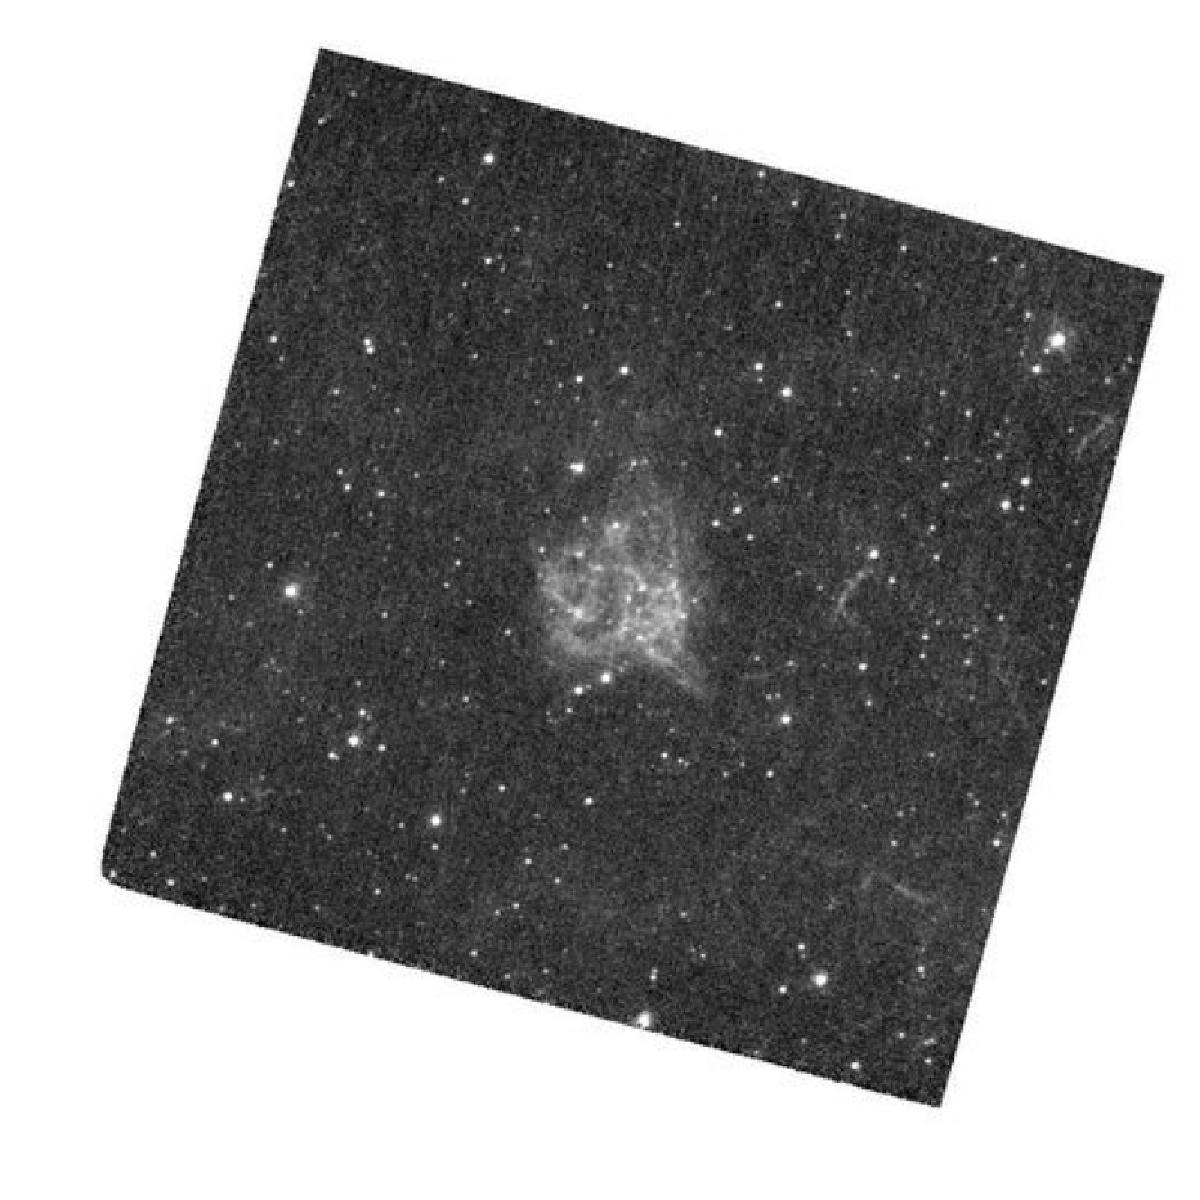
\includegraphics[width=0.18\textwidth]{\thedatafolder/img_2.pdf} & \centering \input{\thedatafolder/cycle_2.txt} \\ (1999) & \centering \input{\thedatafolder/id_2.txt} &  {\scriptsize \input{\thedatafolder/abs1_2.txt}} \tabularnewline
      \midrule
      \centering 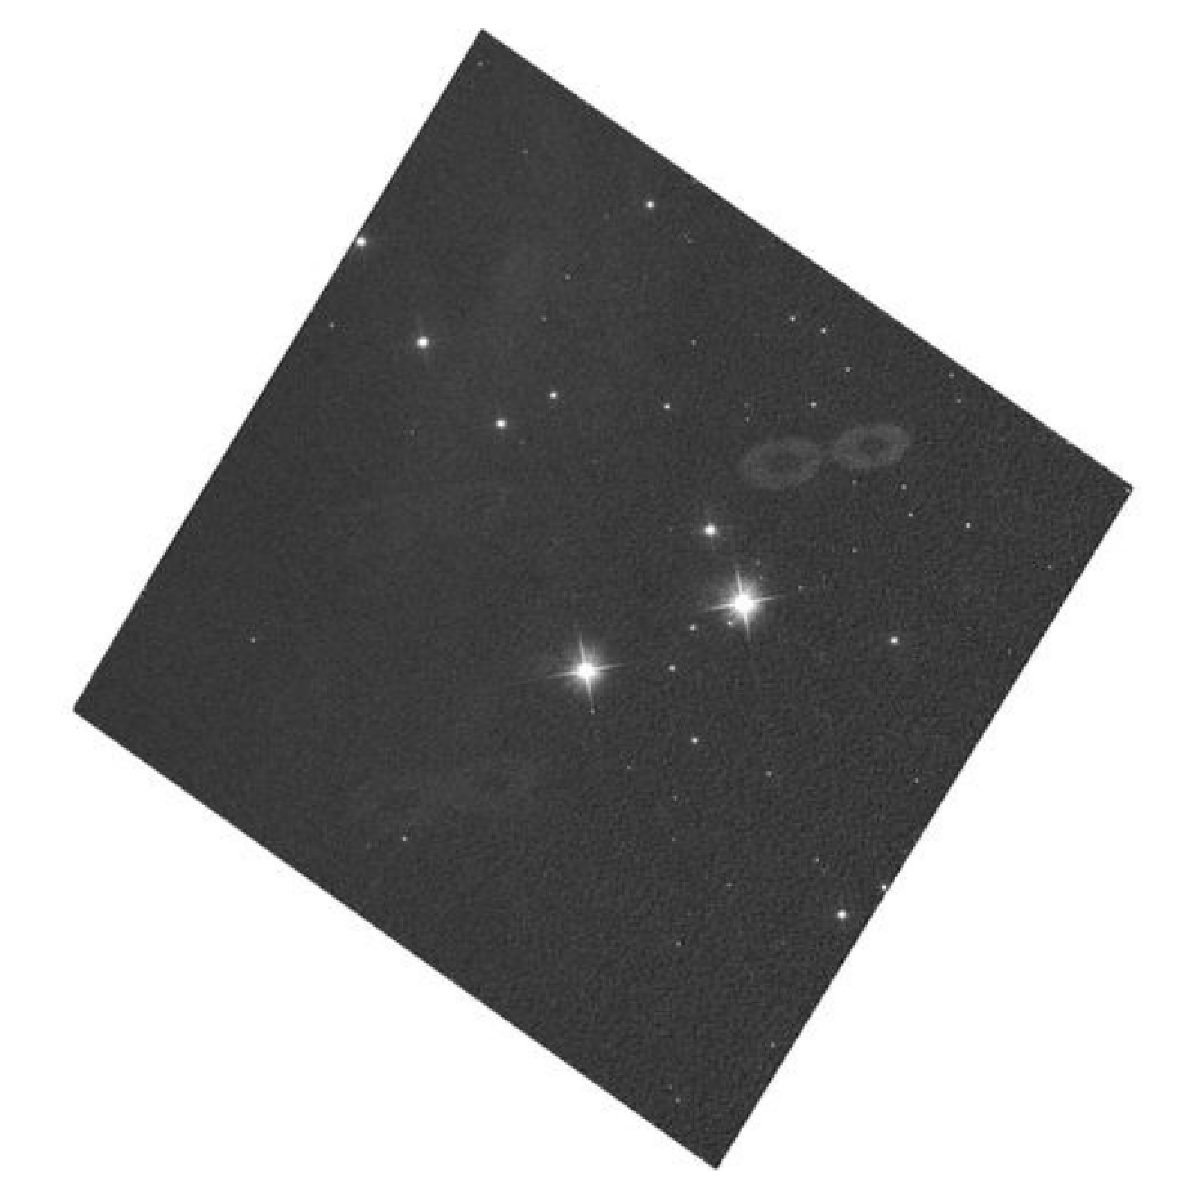
\includegraphics[width=0.18\textwidth]{\thedatafolder/img_1.pdf} & \centering \input{\thedatafolder/cycle_1.txt} \\ (2013) & \centering \input{\thedatafolder/id_1.txt} &  {\scriptsize \input{\thedatafolder/abs1_1.txt}} \tabularnewline
      \midrule
      \centering 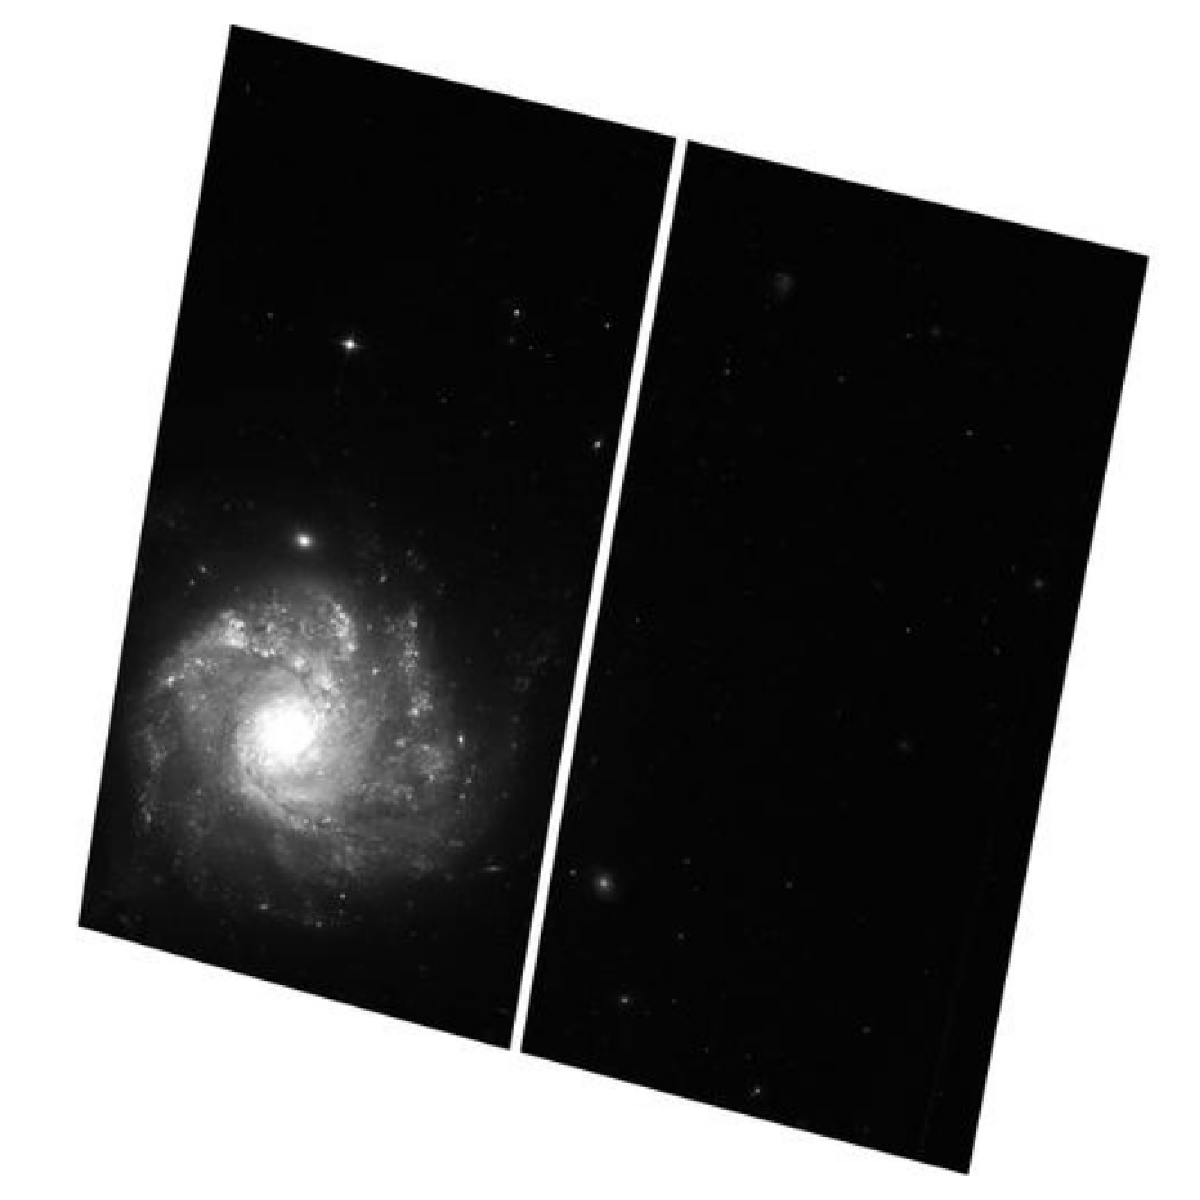
\includegraphics[width=0.18\textwidth]{\thedatafolder/img_3.pdf} & \centering \input{\thedatafolder/cycle_3.txt} \\ (2016) & \centering \input{\thedatafolder/id_3.txt} &  {\scriptsize \input{\thedatafolder/abs1_3.txt}} \tabularnewline
      \midrule
      \centering 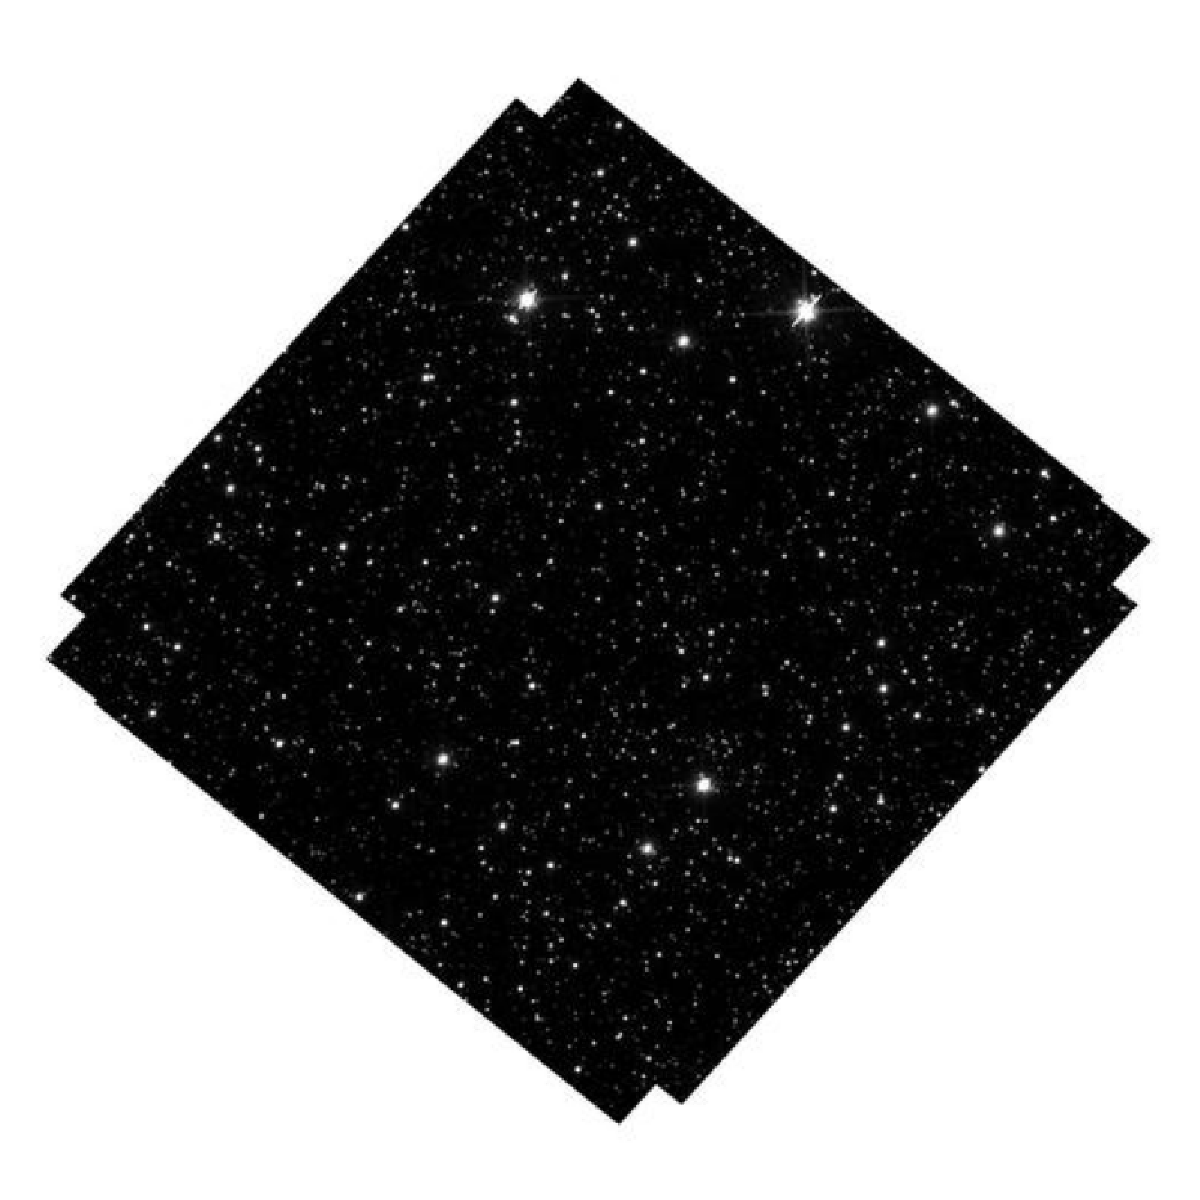
\includegraphics[width=0.18\textwidth]{\thedatafolder/img_0.pdf} & \centering \input{\thedatafolder/cycle_0.txt} \\ (2019) & \centering \input{\thedatafolder/id_0.txt} &  {\scriptsize \input{\thedatafolder/abs1_0.txt}} \tabularnewline
      \bottomrule
  \end{tabular}
  \caption{Examples of \hubble images (left-most column) and corresponding clipped proposal abstracts (right-most column). The observation cycle and corresponding year, as well as proposal ID are shown in the second and third columns, respectively. The proposal ID links to the Mikulski Archive for Space Telescopes (MAST) page corresponding to the proposal.}
  \label{tab:dataset}
\end{table}


\subsection{\hubble Data Selection and Pre-processing}

Observations corresponding to individual proposal IDs are queried through the Mikulski Archive for Space Telescopes (MAST)\footnote{\url{https://mast.stsci.edu/}} via the \package{Astroquery} \citep{2019AJ....157...98G} API.
%
Products of type \texttt{PREVIEW} are filtered in, corresponding to preview postcard images.
%
We note that these are not science-grade observations, but rather lower-resolution images useful for diagnostic purposes.
%
A maximum of 20 images are downloaded per proposal ID, selected at random, in order to avoid biasing the model towards proposals with a larger number of observations and survey-style campaigns.
%
Images are centered and resized to a resolution-per-side of 512 pixels.
%
Color previews (i.e., observations taken with multiple wavelength filters assigned to individual RGB channels) are manually excluded via a filename filter in order to maintain consistency across the dataset; models trained on datasets with color images included were observed to show worse performance on evaluation metrics.
%
If no appropriate images corresponding to an abstract are found, it is excluded from the dataset.

In total 31,859 images corresponding to 4,438 abstracts are included in the fine-tuning dataset.
%
3,194 images are held out for validation, with no abstract being common between training and validation sets in order to ensure an independent set of image-text pairs for evaluation. The held out images correspond to 438 unique abstracts.  % Double check numbers in final version.

We note that some fraction of the image-caption pairs in the constructed dataset will primarily concern instrumentation and/or calibration rather than scientific content.
%
We choose to not filter out these pairs from our dataset, in order to have a larger sample of HST observations that the model can leverage to adapt to the distinctive characteristics of \hubble images.

% Mention that the signal is noisy!

\subsection{Abstract Summarization via Guided Generation}
\label{sec:summarization}

Raw proposal abstracts summarize the corresponding successful HST observing proposals, which intend to make the case for allocating \hubble telescope time towards a particular set of observations.
%
These abstracts are written in a diversity of styles, formats, and lengths while also being highly variable in their content.
%
Although the abstracts can be used as-is as image captions, we experiment with summarizing them via guided large language model (LLM) generation to standardize the captions used for fine-tuning the CLIP model.
%
Captions are summarized by extracting a list of objects and phenomena, as well as potential downstream science use cases, corresponding to the eventual imaged observation.
The intended goal of the summarization process is to increase the strength of the association signal between text and images.

The method from \cite{willard2023efficient} is used to produce an LLM-generated summary of the abstract conforming to a particular schema, specified in JSON format.
%
The schema is designed to represent a list of the objects (e.g., `Type Ia supernova') and phenomena (e.g., `gravitational lensing'), as well as potential downstream science uses cases (e.g., `set constraints on supernova explosion models') that could correspond to the eventual imaged observation given the abstract text, with a minimum of 1 and a maximum of 5 elements per list.

The procedure guides the generation of LLM outputs while ensuring that the schema is respected at every step in the generation process by masking out tokens that would violate the intended format.
%
By framing the problem in terms of transitions between a set of finite states (a finite-state machine), \cite{willard2023efficient} showed that guided generation can be performed with negligible overhead compared to unconstrained generation.
%
See App.~\ref{app:guided-generation} for a more detailed description of the guidance generation method used here.

While the schema-guided generation ensures the \emph{format} of the output, the prompt and choice of LLM will dictate the \emph{content} of the generated summaries.
%
We use the open-weights, instruction-tuned model \textsc{Mixtral-8x7B-Instruct}~\citep{jiang2024mixtral} to generate the summaries, with guided generation performed using the \package{Outlines}\footnote{\url{https://github.com/outlines-dev/outlines}} package.
%
Further details on the summarization procedure, including the prompts and schema used, are provided in App.~\ref{app:summarization}.


The guided generation process ensures that, in this case, the output of the LLM strictly conforms to the format of the following example:
% \SM{Have it be centered}
% \begin{lstlisting}[language=Python]
% {
%   'objects_and_phenomena': ['star forming galaxy', 'lensed galaxy', ...], 
%   'science_use_cases': ['measure lensing magnification', 'probe spectral energy distributions', ...]
% }
% \end{lstlisting}
\begin{center}
  \begin{jsoncode}
    \centering
          \color{black}\{
            \color{codegreen}'objects_and_phenomena'\color{black}: [\color{codegreen}'star forming galaxy', 'lensed galaxy'\color{black}], 
            \color{codegreen}'science_use_cases'\color{black}: [\color{codegreen}'measure lensing magnification'\color{black}]
          \color{black}\}
  \end{jsoncode}
  \end{center}
which is then used to construct the summarized caption by combining the two key elements.
%
Examples of raw abstract snippets and corresponding LLM-generated summaries are shown in Tab.~\ref{tab:datasetsumm}.
%
% We emphasize that the intended goal of summarization-via-guided-generation is to increase the signal between text and images by standardizing the captions used for fine-tuning the CLIP model, and compare the quantitative performance of the model vs using the raw abstracts in Sec.~\ref{sec:results}.
%
We train separate models using the raw abstracts and the LLM-generated summaries, and compare their performance on downstream tasks in Sec.~\ref{sec:results}.
%
We note that, even after summarization, the association signal is expected to be noisy, since aspects of the summarized caption may not be directly descriptive of the observed images.

% Finally, in order to test a further compression of the proposal abstracts, we use LLM-guided generation to also produce a list of single-concept summaries (e.g., `irregular galaxy', `quasars', `Galactic bulge', \ldots), and test whether this can lead to meaningful, generalizable learned associations with observations.
% %
% The prompts and schemata for generating these discrete categories and assigning observations to them are described in Apps.~\ref{app:singleconcept} and \ref{app:singleconceptassignments} respectively. \SM{Each abstract is assigned one summary. The generation of the single concepts is different }


\begin{landscape}
  \begin{table}[h!]
    \renewcommand{\arraystretch}{2}
      \centering
      \begin{tabular}{m{1.8cm} m{8cm} m{5cm} m{6.5cm}}
          \toprule
          \bfseries Prop. ID & \centering\arraybackslash \bfseries Proposal abstract & \multicolumn{2}{c}{\bfseries LLM-extracted summary} \tabularnewline
          \cmidrule(r){3-4}
          & & \centering\arraybackslash \bfseries Objects and phenomena & \centering\arraybackslash \bfseries Science use cases \tabularnewline
          \midrule
          \input{\thedatafolder/id1_2.txt} & {\scriptsize \input{\thedatafolder/abs1_2.txt}} & {\scriptsize \input{\thedatafolder/obj1_2.txt}} & {\scriptsize \input{\thedatafolder/sci1_2.txt}} \tabularnewline
          \midrule
          \input{\thedatafolder/id1_1.txt} & {\scriptsize \input{\thedatafolder/abs1_1.txt}} & {\scriptsize \input{\thedatafolder/obj1_1.txt}} & {\scriptsize \input{\thedatafolder/sci1_1.txt}} \tabularnewline
          \midrule
          \input{\thedatafolder/id1_3.txt} & {\scriptsize \input{\thedatafolder/abs1_3.txt}} & {\scriptsize \input{\thedatafolder/obj1_3.txt}} & {\scriptsize \input{\thedatafolder/sci1_3.txt}} \tabularnewline
          \midrule
          \input{\thedatafolder/id1_0.txt} & {\scriptsize \input{\thedatafolder/abs1_0.txt}} & {\scriptsize \input{\thedatafolder/obj1_0.txt}} & {\scriptsize \input{\thedatafolder/sci1_0.txt}} \tabularnewline
          \bottomrule
      \end{tabular}
      \caption{Examples of the clipped \hubble proposal abstracts (second column) and LLM (\textsc{Mixtral-8x7B})-extracted summaries (right-most two columns), separately extracting objects and phenomena as well as potential downstream science use cases. \SM{Don't rotate?}}
      \label{tab:datasetsumm}
  \end{table}
  \end{landscape}



\section{Methodology}
\label{sec:methodology}

Our goal is to learn a semantically meaningful joint representation between images corresponding to HST observation and natural (English) language.
%
With PAPERCLIP, we leverage the strong generalization capabilities demonstrated by pre-trained CLIP models and adapt these to work with domain-specific \hubble data via fine tuning.

\subsection{Contrastive Language-Image Pre-training (CLIP)}

CLIP \citep[Contrastive Language-Image Pre-training;][]{radford2021learning} is a multi-modal neural network model pre-trained on a large corpus of image-text pairs via weak supervision using a contrastive loss.
%
Given a minibatch $\mathcal{B}$ of $|\mathcal{B}|$ image-text pairs $\{(I_i, T_i)\}$, the goal is to align the learned representations of corresponding (positive) pairs $(I_i, T_i)$ while repelling the representations of unaligned (negative) pairs $(I_i, T_{j\neq i})$.
%
Image and text encoders $f: I \rightarrow \mathbb R^{n_\text{emb}}$ and $g: T \rightarrow \mathbb R^{n_\text{emb}}$ are used to map images and text to a common embedding space of dimension $n_\text{emb}$.
%
We use the standard softmax-based bidirectional variant of the InfoNCE~\citep{oord2018representation} contrastive loss function introduced for training CLIP-style architectures \citep{radford2021learning}
%
\begin{equation}
  \label{eq:softmax_loss}
  \mathcal{L}(\mathcal{B})=-\frac{1}{2|\mathcal{B}|} \sum_{i=1}^{|\mathcal{B}|}\left(\log \frac{e^{x_i \cdot y_i / \tau}}{\sum_{j=1}^{|\mathcal{B}|} e^{x_i \cdot y_j / \tau}}+\log \frac{e^{x_i \cdot y_i / \tau}}{\sum_{j=1}^{|\mathcal{B}|} e^{x_j \cdot y_i / \tau}}\right)
\end{equation}
%
where ${x}_i={f\left(I_i\right)}/{\left\|f\left(I_i\right)\right\|}$ and ${y}_i={g\left(T_i\right)}/{\left\|g\left(T_i\right)\right\|}$ are the normalized representations of the $i$-th image and text, respectively, and $\tau$ is a learnable temperature hyperparameter.
%
Note that this loss treats the image and text representations symmetrically, ensuring that the two modalities are on the same footing.

We use the CLIP-ViT-B/16\footnote{\url{https://huggingface.co/openai/clip-vit-base-patch16}} \citep{radford2021learning} variant as the base pre-trained CLIP model.
%
This model uses a 12-layer, 12-head, 768-embedding dimension vision transformer as the image encoder and a 12-layer, 8-head, 512-embedding dimension sequence transformer as the text backbone.
%
The text encoder has a maximum length of 77 tokens and the image encoder a native resolution of $224\times224$ pixels.
%
Linear projection layers map the outputs of the image and text encoders to a common embedding space of dimension $n_\text{emb}=512$.
%
In total, the model has 149,620,737 trainable parameters.
%
This model was originally pre-trained on 400 million image-text pairs from internet data \citep{radford2021learning}.
%

\subsection{Fine-tuning Procedure}

The base CLIP model is fine-tuned using the dataset described in Sec.~\ref{sec:dataset}, using either the LLM-summarized abstracts or raw proposal abstracts.
%
When using raw proposal abstracts, random chunks of the text delimited by periods are selected on the fly to fit within the maximum token length of the text encoder.
%
Images are augmented via random four-fold rotations (increments of $90^\circ$) and randomly cropped to the native resolution of the image encoder, maintaining $\sim 20\%$ of the area of the original image, at each training step.
%
Given the relatively modest size of the fine-tuning dataset, a batch size $|\mathcal B| = 32$ is used throughout; larger batch sizes were observed to be susceptible to overfitting.
%
The temperature hyperparameter $\tau$ was initialized to its pre-trained value.
%
We emphasize that the positive and negative image-text association is noisy and imperfect, since multiple images can be associated with the same abstract, and the goal of the fine-tuning process is to leverage the signal contained in this noisy association. 

We explore three different methods of training the model on our domain dataset: \emph{(1)} Fine-tuning the entire network starting from the pre-trained base model; \emph{(2)} Freezing the base image/text encoders and training a small projection head; and \emph{(3)} Training the entire model from scratch.
%
For \emph{(2)}, we use a 2-layer MLP with 1024 hidden units and a GELU activation layer, projecting onto the 512-dimensional common embedding space.

All models were trained over 20,000 steps with 2000 linear warmup steps 
% and cosine decay 
using the AdamW optimizer \citep{DBLP:conf/iclr/LoshchilovH19,DBLP:journals/corr/KingmaB14} with  %peak 
learning rate $10^{-5}$ and weight decay $10^{-3}$.
%
Training takes approximately 3 hours on 4 Nvidia A100 GPUs.
Models were instantiated using the \package{Transformers} \citep{wolf2019huggingface} library and trained using packages from the \package{Jax} \citep{jax2018github} ecosystem.
%


\subsection{Evaluation Metrics}
\label{sec:eval}

The model is evaluated by tracking the contrastive loss in Eq.~\eqrefb{eq:softmax_loss} as well as the top-$k\%$ retrieval accuracy on the held out validation set over the course of training.
%
The retrieval accuracy is defined as the fraction of associated captions which fall within the top $k\%$ of captions by cosine similarity of the normalized image and caption embeddings, averaged over the images in the validation set:
\begin{equation}
\text{Retrieval accuracy}_k = \frac{1}{|\mathcal V|} \sum_{i=1}^{|\mathcal V|} \mathbbm{1}\left[\operatorname{rank}\left({x}_i \cdot {y}_{i}; \{{x}_i \cdot {y}_{j}\}_{j=1}^{|\mathcal V|}\right) \leq \left\lfloor\frac{k}{100}|\mathcal V|\right\rfloor\right]
\label{eq:retrieval_accuracy}
\end{equation}
where $|\mathcal V|$ is the total number of images in the validation set, $\mathbbm{1}(\cdot)$ is the indicator function that returns 1 if the condition inside the brackets is true and 0 otherwise, $\operatorname{rank}\left({x}_i \cdot {y}_{i}; \{{x}_i \cdot {y}_{j}\}_{j=1}^{|\mathcal V|}\right)$ is a function that returns the rank of the cosine similarity between ${x}_i$ and ${y}_{i}$ among the cosine similarities between ${x}_i$ and all captions ${y}_j$ in the validation set, and $k$ is the percentage of top captions considered for the retrieval accuracy. Note that this metric is symmetric in the image and text modalities.

We also qualitatively evaluate the learned embeddings through image retrieval (i.e., retrieving the most relevant images from the validation set using natural language queries) and description retrieval (i.e., querying the astrophysical object classes and science use cases most relevant to a given observation, akin to zero-shot classification) experiments. 
%
For the description/text retrieval evaluation, we curate a list of possible text associations (i.e., classes) by querying the \textsc{Claude 2}\footnote{\url{https://claude.ai/}} large language model, which we show in App.~\ref{app:categories}.

\section{Results and Discussion}
\label{sec:results}

\subsection{Quantitative Evaluation}

\paragraph*{Validation metrics during training}

Figure~\ref{fig:retrieval_acc} shows the contrastive loss (left) and the top-10\% retrieval accuracy (right) evaluated on the held out validation set over the course of training, for different training configurations considered.
%
The dashed orange lines show the metrics evaluated when training with batches where the image-text associations are randomly shuffled.
%
This randomized baseline is seen to do on par with random expectation (i.e., a 10\% retrieval accuracy), unlike the others, validating the presence of a significant association signal between images and text in the dataset.
%
Interestingly, the base pre-trained model performs better than random expectation, with a top-10\% retrieval accuracy of $\sim 15\%$.
%
We therefore also compare the qualitative performance of the base model with the fine-tuned models on downstream retrieval tasks.

The model trained using LLM-summarized abstracts (red lines) is seen to perform slightly worse than the model using raw abstracts as captions (blue lines), despite the curation of the summarized-abstract dataset intended to provide a stronger image-text association signal.
%
Fine-tuning a small MLP head over frozen vision and text backbones (dotted green lines) and training from scratch (yellow lines) show a non-trivial improvement compared to the base model, although with deteriorated performance compared to fine-tuning with either summarized or raw abstracts.

\begin{figure*}[!h]
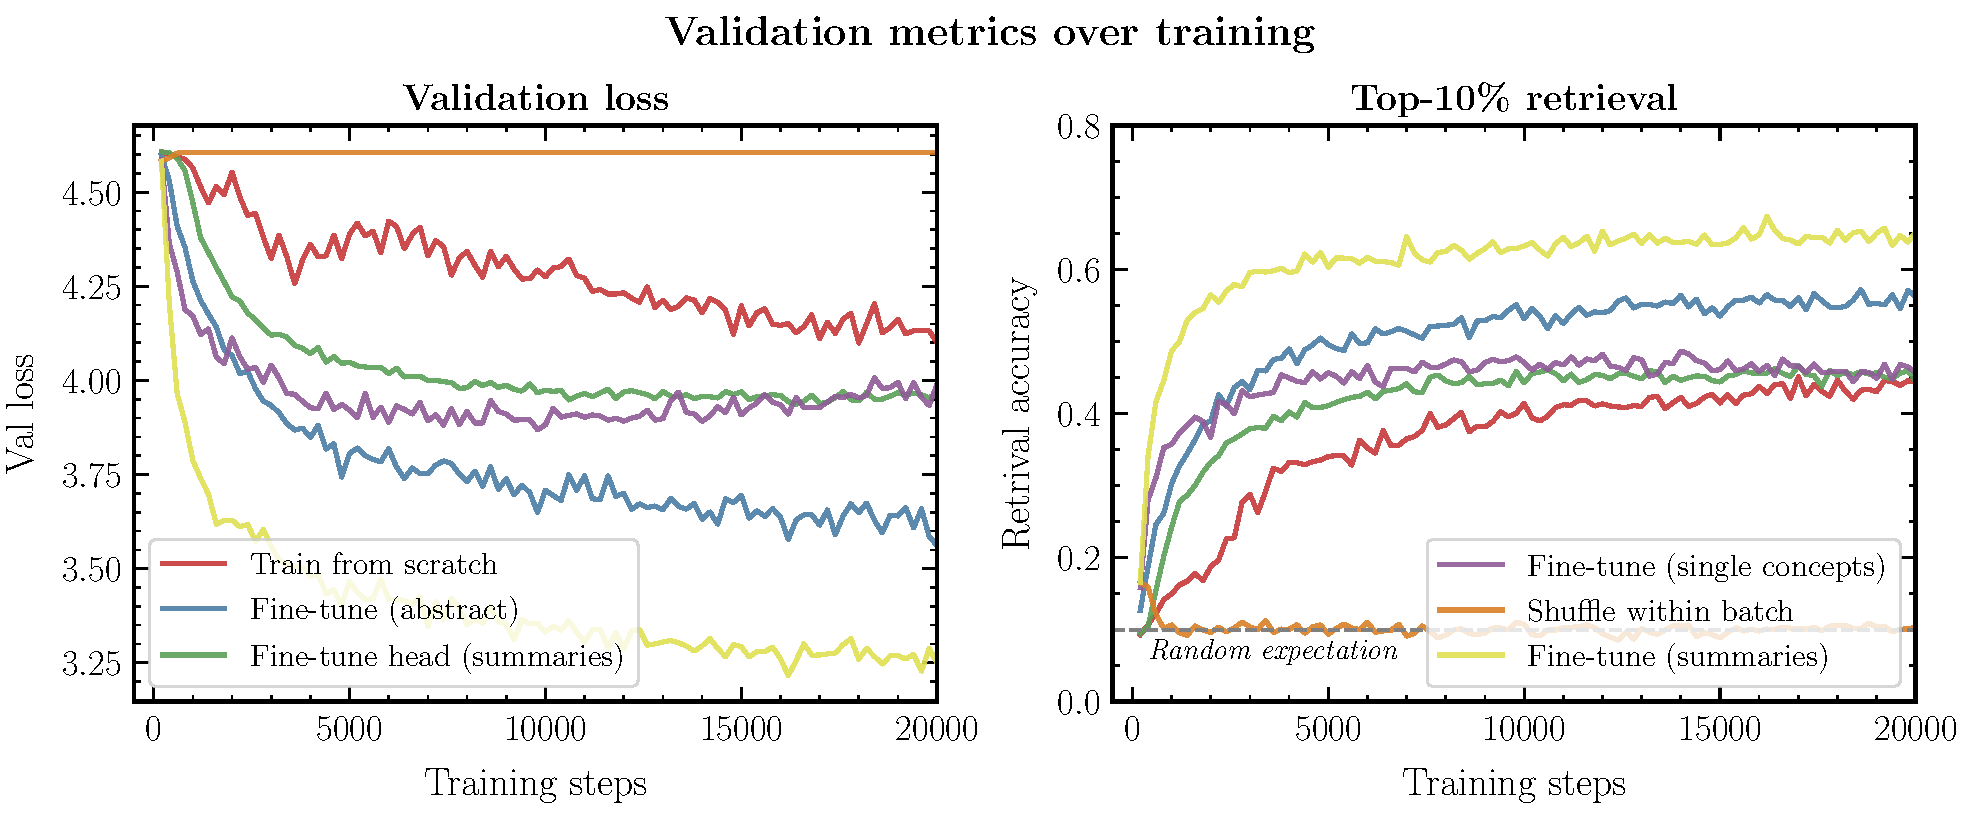
\includegraphics[width=0.99\textwidth]{plots/val_metrics.pdf}
\caption{The CLIP contrastive loss from Eq.~\eqrefb{eq:softmax_loss} (left) and the top-10\% retrieval accuracy from Eq.~\eqrefb{eq:retrieval_accuracy} (right) computed on the validation set over the course of training. Shown for the dataset with summarized abstracts as captions (red), dataset using raw proposal abstracts as captions (blue), only fine-tuning a small MLP head (dotted green), training from scratch (purple), and trained with shuffled image-text pairs (dashed orange).} 
\label{fig:retrieval_acc}
\end{figure*}

\paragraph*{Distribution of text-image cosine similarities}

Figure~\ref{fig:sim_valtrain} (left) shows the distribution of cosine similarities between corresponding image and text embeddings, $x_i$ and $y_i$, for the base CLIP model (purple line), and for the LLM-summarized abstracts using the fine-tuned CLIP model (red line).
%
Distributions evaluated for a shuffled order of text embeddings -- therefore randomizing the image-text correspondence during evaluation -- are shown as dashed lines. We note that the shuffling here is performed at the evaluation stage, and not the training stage.
%
The distributions for the base model is seen to be sharply peaked at a specific value, showing little diversity and being very similar between the shuffled (dashed purple) and non-shuffled (solid purple) versions. 
%
Distributions for the fine-tuned model, on the other hand, show a clear separation when evaluated on shuffled (dashed red) and corresponding (solid red) text-image pairs.

% Similarly, Fig.~\ref{fig:sim_valtrain} (top right) shows the distribution of cosine similarities between corresponding image-text pairs for the single-concept captions (solid red) and the shuffled versions (dashed red).
% %
% The distribution for corresponding pairs is only modestly shifted compared to the shuffled version, indicating that assigning $\mathcal O(400)$ labels to the images using an LLM results in a weaker association signal compared to using noisy captions.
% %
% The purple line shows the distribution of cosine similarities between corresponding pairs with single-concept summaries, but evaluated using a model trained on the LLM-summarized abstracts.
% %
% This distribution is more skewed towards higher similarity values, indicating that the model trained on diverse caption can still better capture the association signal in the single-concept summaries compared to one trained specifically using the single-concept summaries.

\paragraph*{Retrieval accuracy}

Figure~\ref{fig:sim_valtrain} (right) shows the retrieval accuracy, as defined in Eq.~\eqrefb{eq:retrieval_accuracy}, as a function of the retrieval fraction $k$.
%
In this case, we evaluate all four models (fine tuned on raw abstracts (blue), fine-tuned on LLM-summarized abstracts (red), trained on LLM-summarized abstracts from scratch (yellow), and the base model (purple)) on the same captions dataset, the summarized abstracts, for a direct comparison.
%
Remarkably, the model trained on raw abstracts shows very similar performance when evaluated on the summarized abstracts compared to that trained on the summarized abstracts themselves, indicating that \emph{(1)} the image-text association signal is preserved in the summarization process, and \emph{(2)} the model is able to effectively leverage meaningful concepts in the noisy raw abstracts through weak supervision.

\begin{figure*}[!h]
  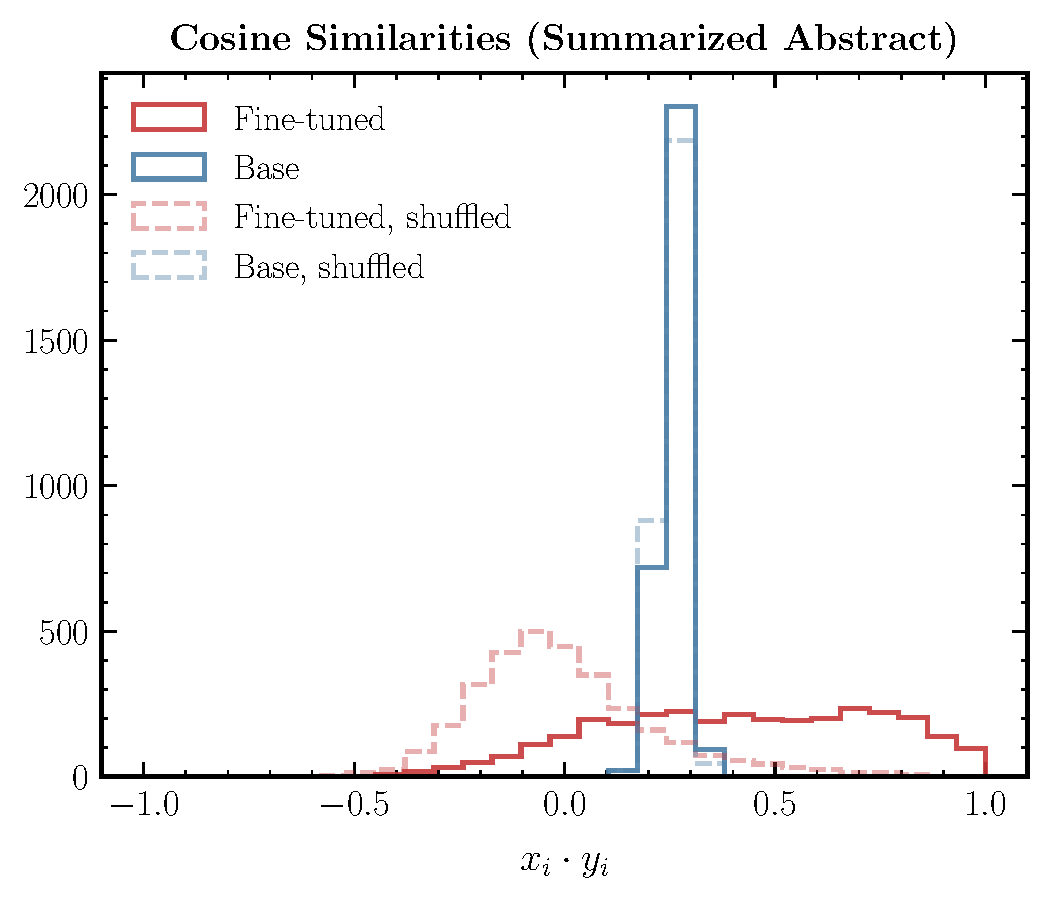
\includegraphics[width=0.49\textwidth]{plots/sim_val.pdf}
  % 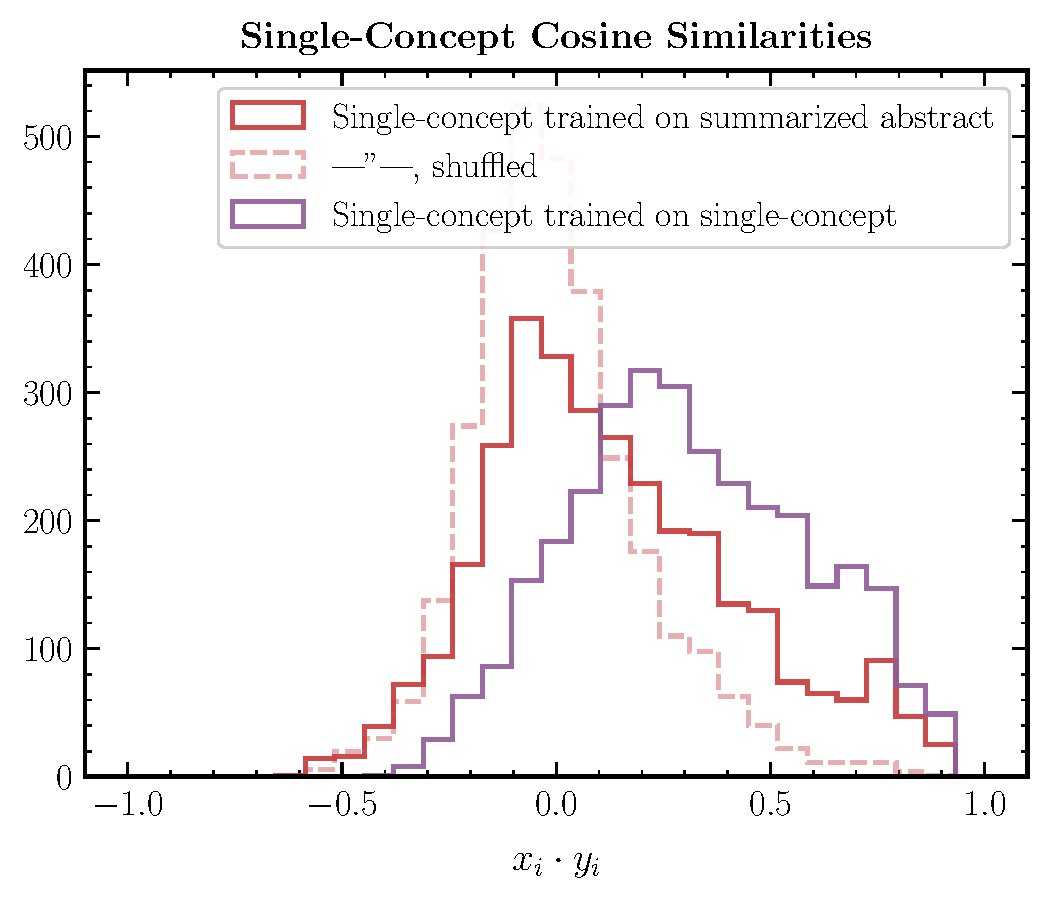
\includegraphics[width=0.45\textwidth]{plots/sim_summ1.pdf}
  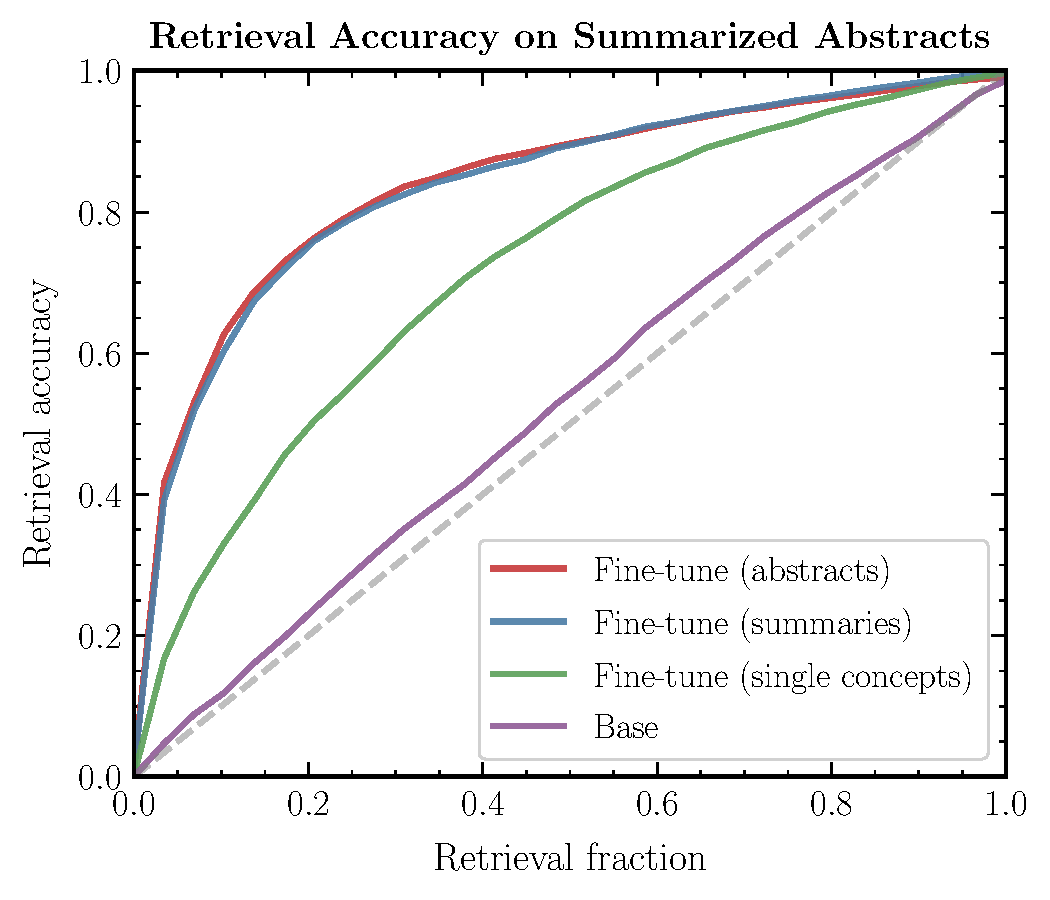
\includegraphics[width=0.49\textwidth]{plots/retrieval.pdf}
  \caption{(Left) Distribution of cosine similarities between corresponding image and text embeddings, $x_i$ and $y_i$, shown when using the base CLIP model (purple lines), and the summary fine-tuned CLIP model (red line). Dashed lines correspond to models evaluated on image-text pairs with associations shuffled. (Right) Retrieval accuracy as a function of the retrieval fraction $k$ for the fine-tuned model on the summarized abstracts (red), fine-tuned on raw abstracts (blue), trained on LLM-summarized abstracts from scratch (yellow), and the base model (purple).}
  \label{fig:sim_valtrain}
  \end{figure*}

\subsection{Image Retrieval}

Having aligned the image and text representations, we can embed a natural language query using the model and show the closest images by embedding when ranked by cosine similarity.
%
We show these in Tabs.~\ref{tab:tti_base} and \ref{tab:tti} for the base and fine-tuned models respectively using four simple curated queries: \texttt{dwarf galaxy} (small galaxies that typically orbit larger galaxies like the Milky Way), \texttt{Jupiter},  \texttt{SN1987A} (a specific, prominent supernova), and \texttt{strong lensing} (the phenomenon of bending of light due to the gravitational influence of a foreground distribution of matter). The proposal ID corresponding to the retrieved images is shown below each image, which contains a hyperlink to the MAST page corresponding to the proposal.

While the base model shows some signs of meaningful retrieval (e.g., the image of Jupiter in the second row of Tab.~\ref{tab:tti_base}, and images of galaxies in first row), it is challenging to discern meaningful, strong associations between the retrieved images and corresponding query.

The model fine-tuned with summarized abstracts (Tab.~\ref{tab:tti}), meanwhile, shows strikingly different behavior.
%
% For example, it is able to return images with processing and assembly artifacts particular to HST (e.g., the lines through the middle in some images), which typically receive low similarity scores when using the base model.
%
Images of Jupiter are returned for the \texttt{Jupiter} query, with the planet clearly visible in all four images.
%
The \texttt{dwarf galaxy}-queried images correspond to proposals aiming to measure the kinematics of the stellar cores of dwarf galaxies.
%
Supernova SN1987 itself can be seen in the three closest images for the \texttt{SN1987A} query with the fourth image being a supernova remnant.
%
Cluster-scale as well as galaxy-scale gravitational lenses are returned by the \texttt{strong lensing} query, with lensing patterns visible in the images.

\subsection{Text Retrieval}

We can use images from the validation set as queries and retrieve the most relevant text chunks (e.g., objects and use cases) from a curated list as described in Sec.~\ref{sec:eval}.
%
We show the result of image-to-text retrieval in Tab.~\ref{tab:itt}, for the base (second column) as well as summary fine-tuned (third column) models, using four observations (left-most column) from the validation set.
% %
% We curate a list of possible text associations by querying the \textsc{Claude}\footnote{\url{https://claude.ai/}} large language model for such a list, which we show in App.~\ref{app:categories}.

The top four text associations are shown for each image query.
%
The `ground truth' summarized abstract is shown in the right column.
% 
The base as well as fine-tuned models are seen to return a mix of relevant and less-relevant associations, although showing different qualitative behavior. Purely qualitatively, the fine-tuned model is seen to consistently return more relevant associations compared to the base model.
%

The second row (an image of supernova 1987A) highlights an interesting pattern -- the base model erroneously attributes the object at the center of the image to a gravitational lens, while the fine-tuned model correctly identifies it as a supernova remnant.

Note that we chose to illustrate qualitative performance on text and image retrieval using the model fine-tuned on summarized abstracts, rather than raw abstracts. We show analogous results for the model fine-tuned on raw abstracts in App.~\ref{app:eval_raw}. Although the two models show very similar quantitative performance on retrieval metrics (as shown in Fig.~\ref{fig:sim_valtrain}), they exhibit characteristic behavior in terms of objects (images/text) retrieved. We emphasize that for scientific usefulness, the most useful goal is not necessarily to retrieve the objects with the highest similarity scores, but rather to identify a diverse set of interesting candidates for manual follow-up and further analysis; both models are seen to perform sensibly, even if differently, in this regard.


\begin{table}[h!]
  \centering
  \begin{tabular}{m{3cm} p{3cm} p{3cm} p{3cm} p{3cm}}
      \toprule
      \centering \bfseries Query & \multicolumn{4}{c}{\bfseries{Top-4 most similar images using \textcolor{deeppurple}{base CLIP model}}} \tabularnewline
      \midrule
      \texttt{\input{\thedatafolder/query_tti_base_1.txt}} \vspace{20mm} & \centering 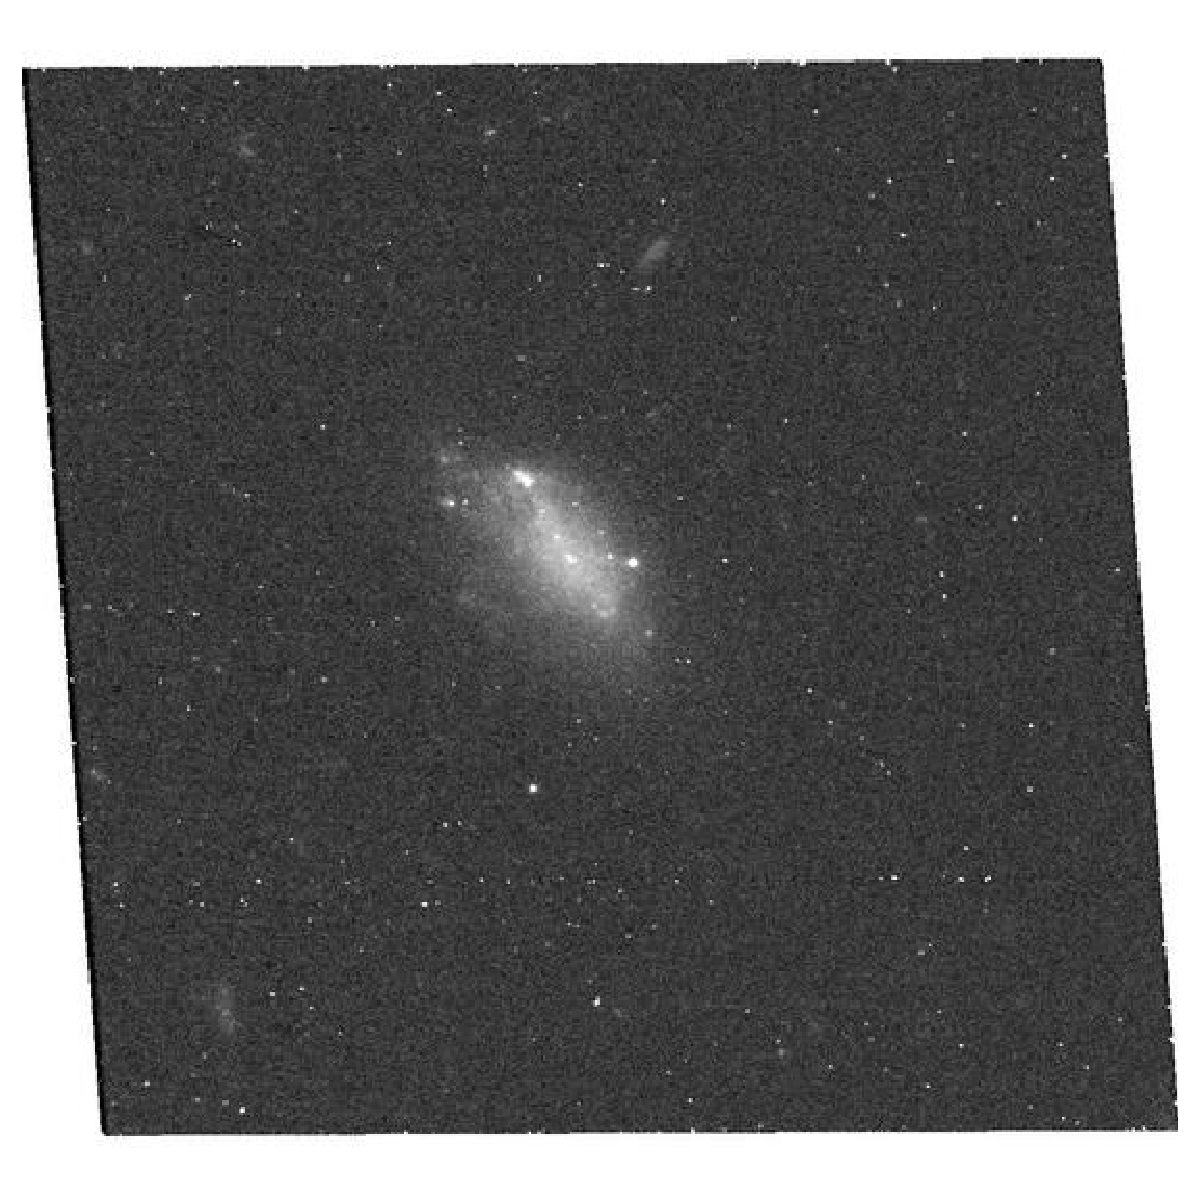
\includegraphics[width=0.18\textwidth]{\thedatafolder/img_tti_base_1_0.pdf} \\ \input{\thedatafolder/propid_tti_base_1_0.txt} & \centering 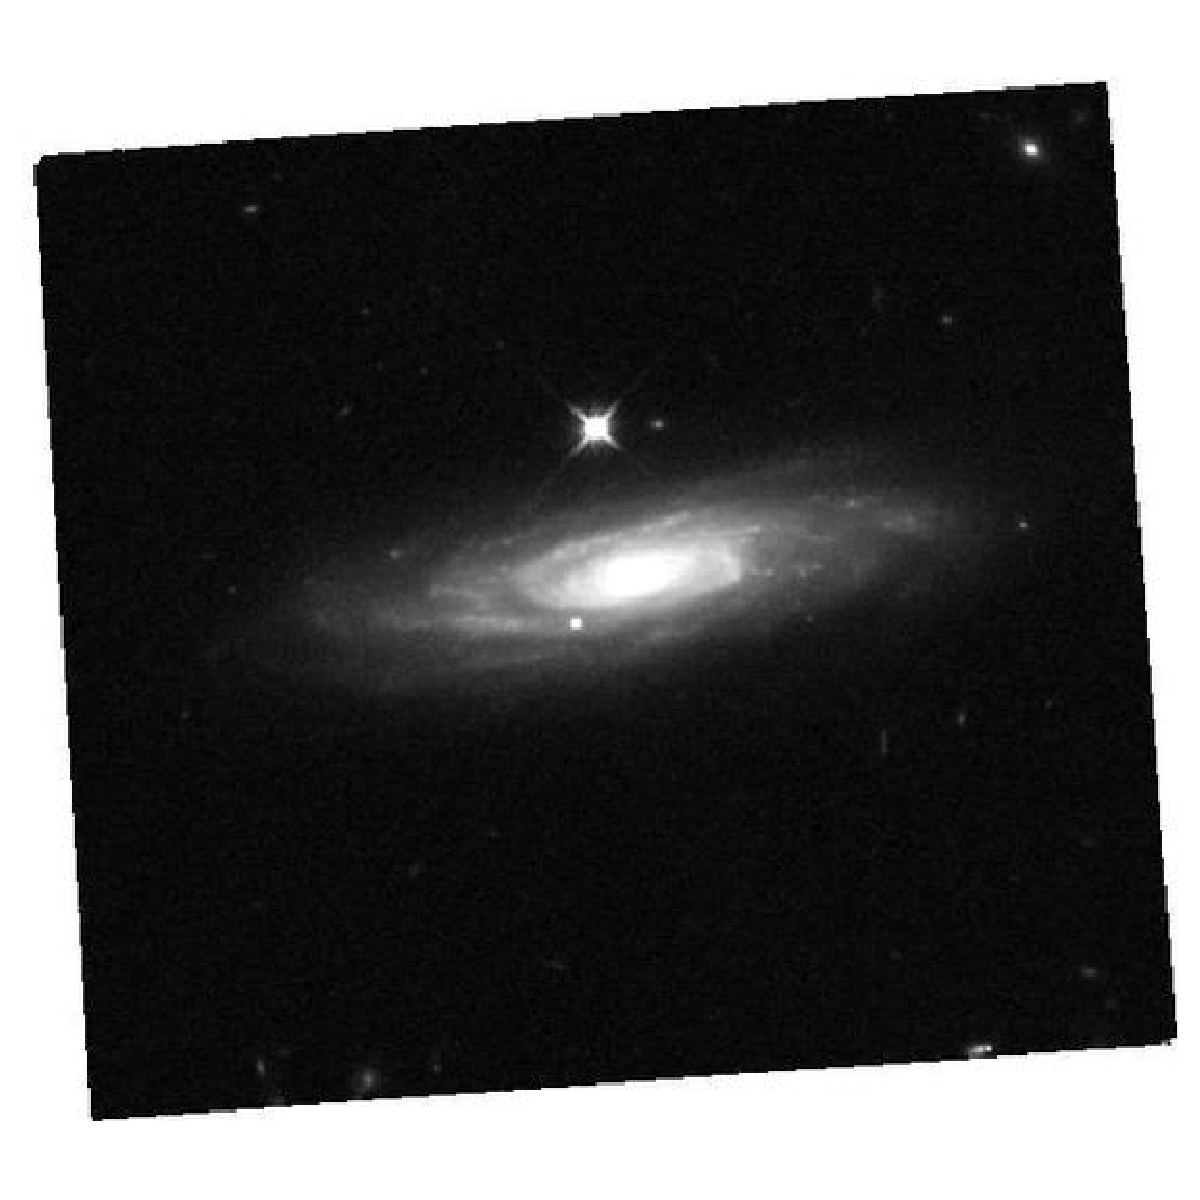
\includegraphics[width=0.18\textwidth]{\thedatafolder/img_tti_base_1_1.pdf} \\ \input{\thedatafolder/propid_tti_base_1_1.txt} & \centering 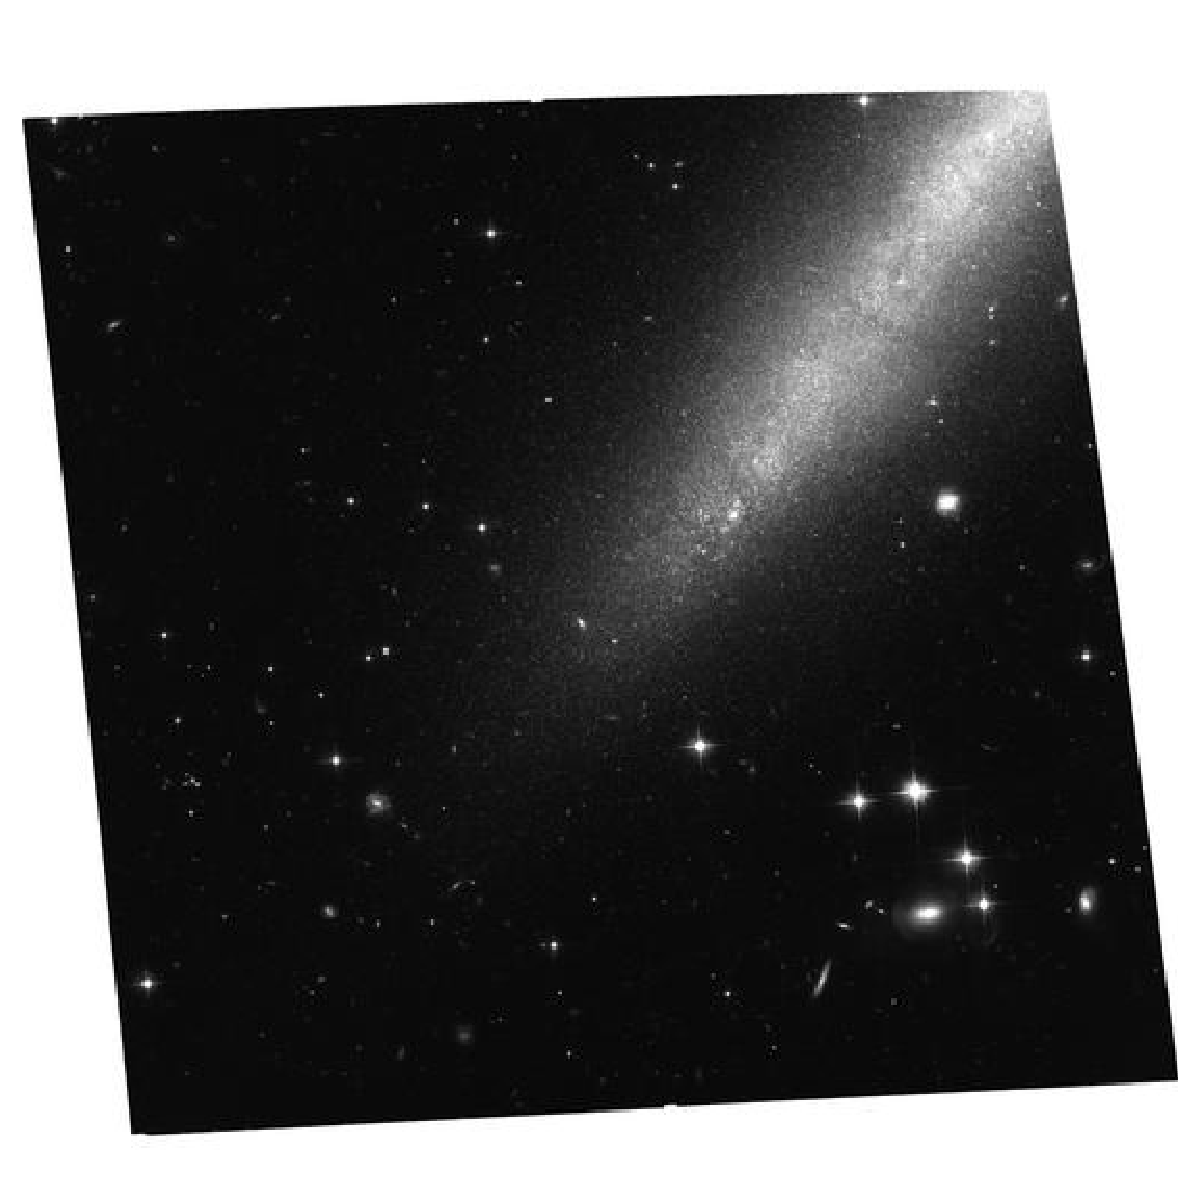
\includegraphics[width=0.18\textwidth]{\thedatafolder/img_tti_base_1_2.pdf} \\ \input{\thedatafolder/propid_tti_base_1_2.txt} & \centering 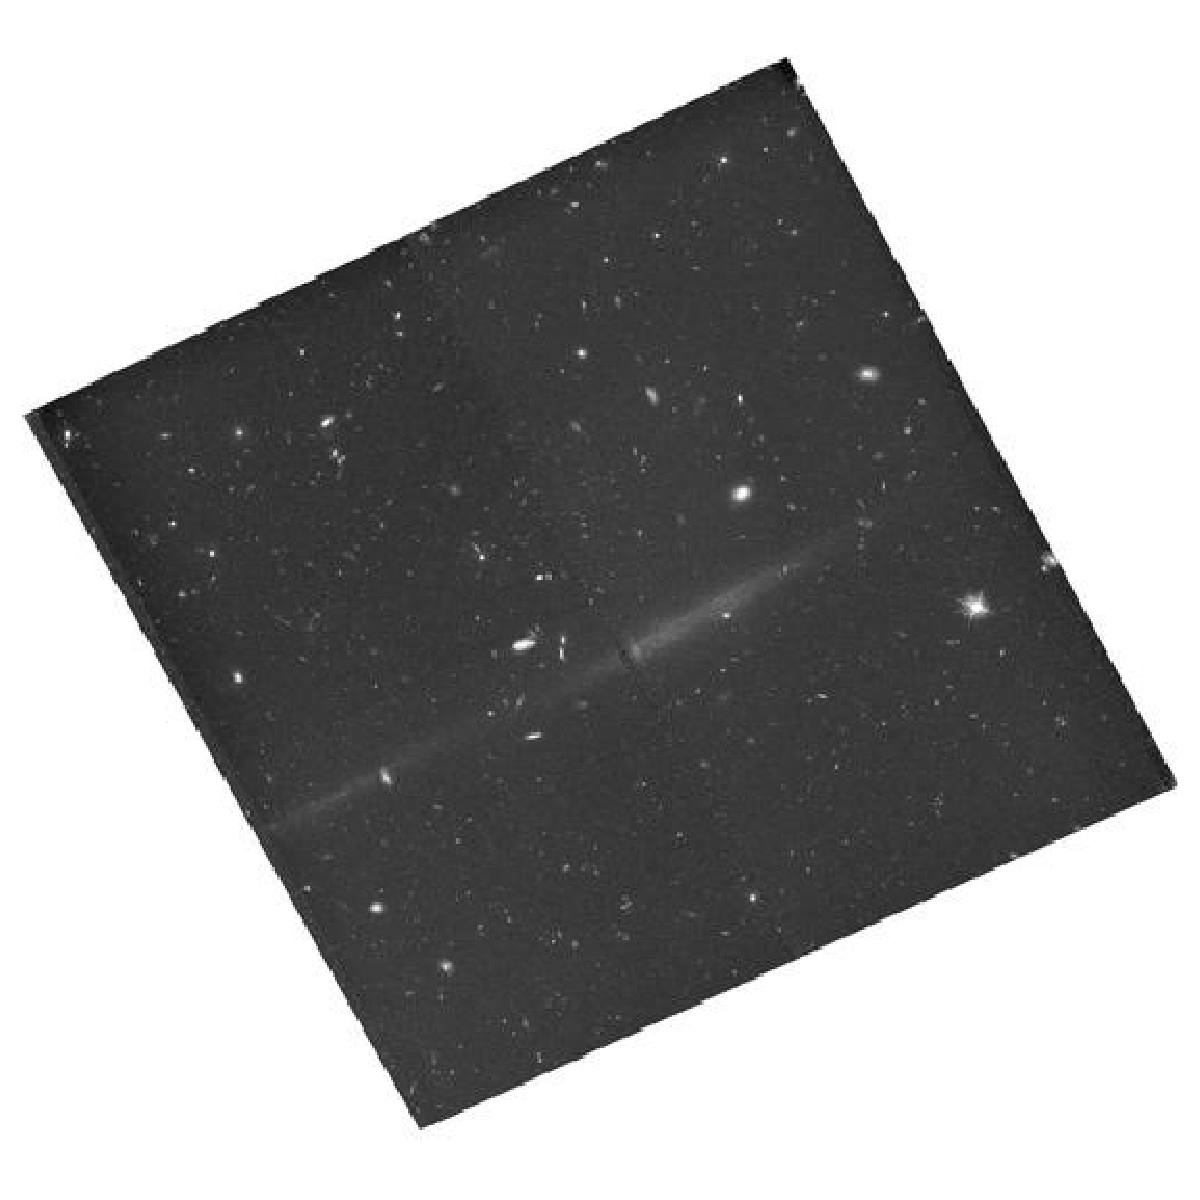
\includegraphics[width=0.18\textwidth]{\thedatafolder/img_tti_base_1_3.pdf} \\ \input{\thedatafolder/propid_tti_base_1_3.txt}  \tabularnewline
      \midrule
       \texttt{\input{\thedatafolder/query_tti_base_0.txt}} \vspace{20mm} & \centering 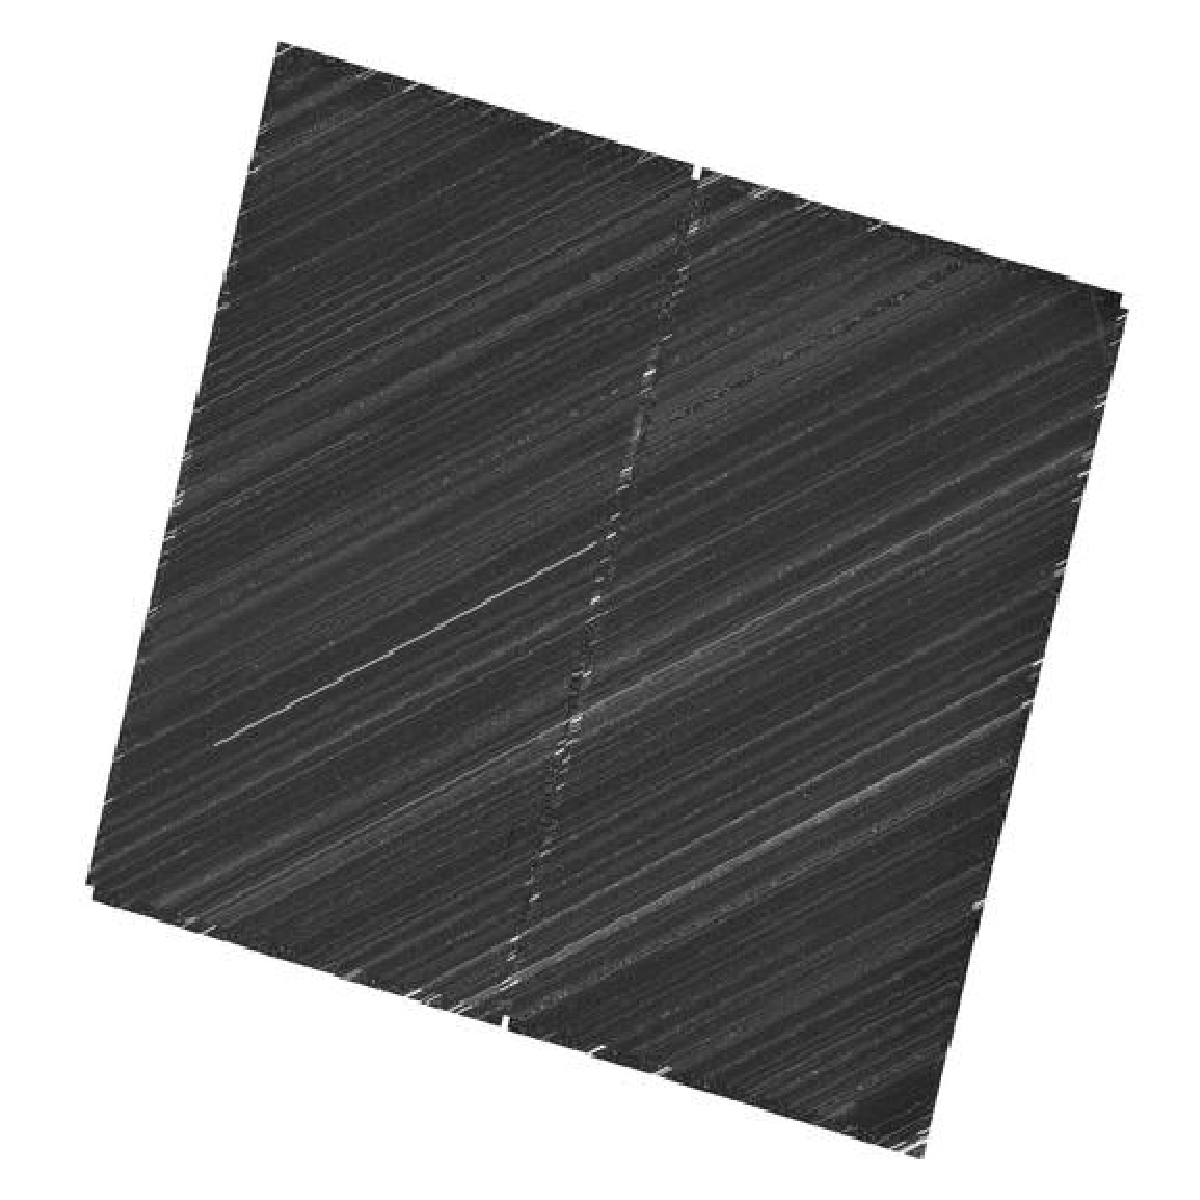
\includegraphics[width=0.18\textwidth]{\thedatafolder/img_tti_base_0_0.pdf} \\ \input{\thedatafolder/propid_tti_base_0_0.txt} & \centering 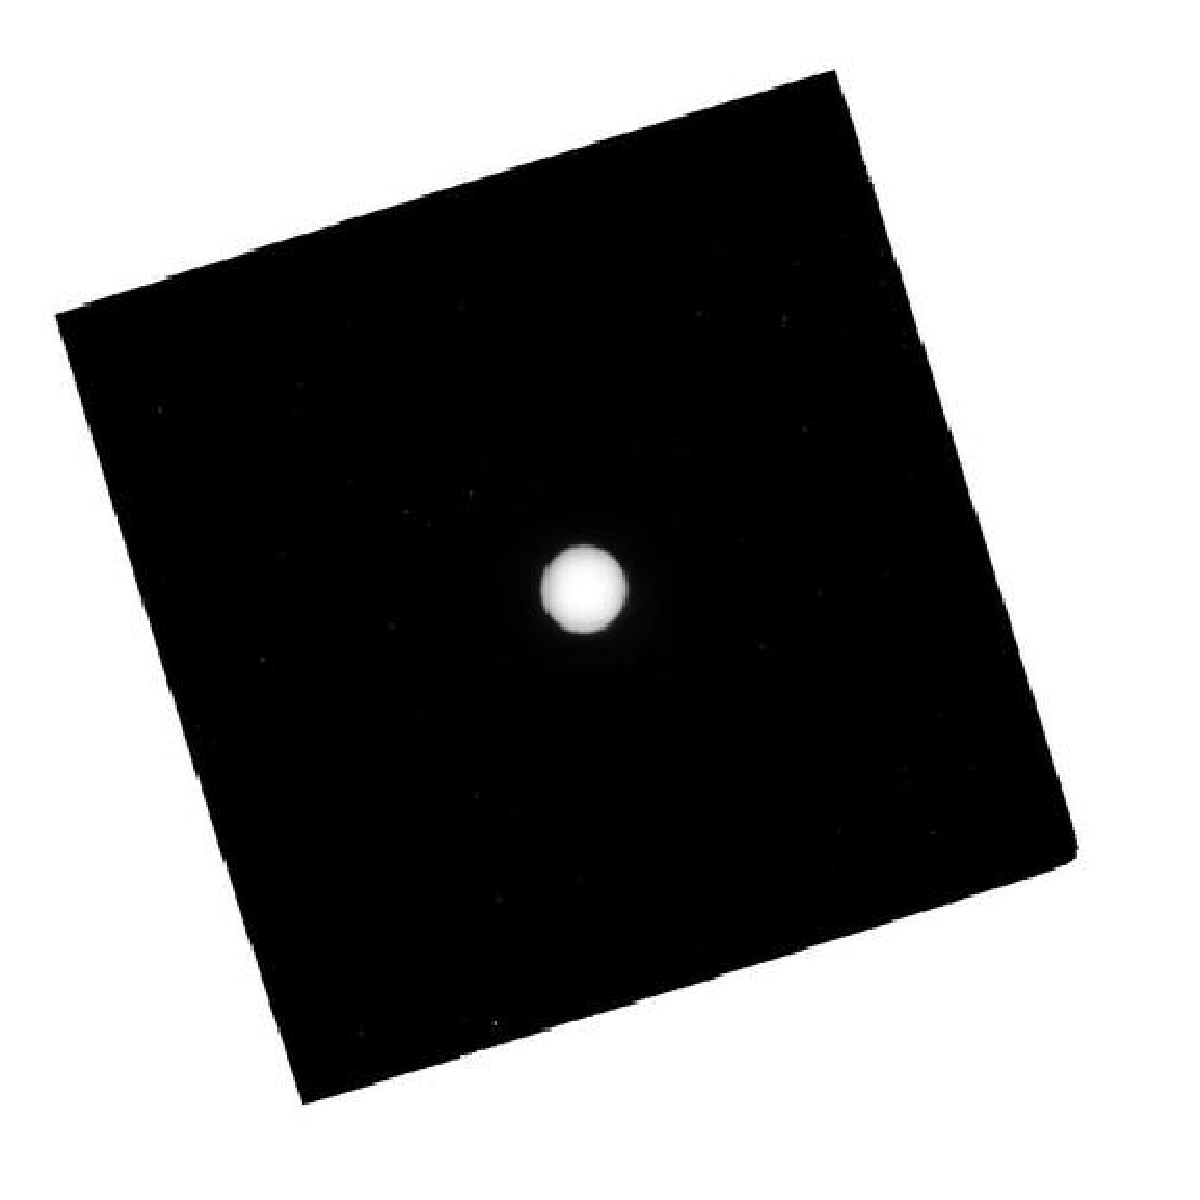
\includegraphics[width=0.18\textwidth]{\thedatafolder/img_tti_base_0_1.pdf} \\ \input{\thedatafolder/propid_tti_base_0_1.txt} & \centering 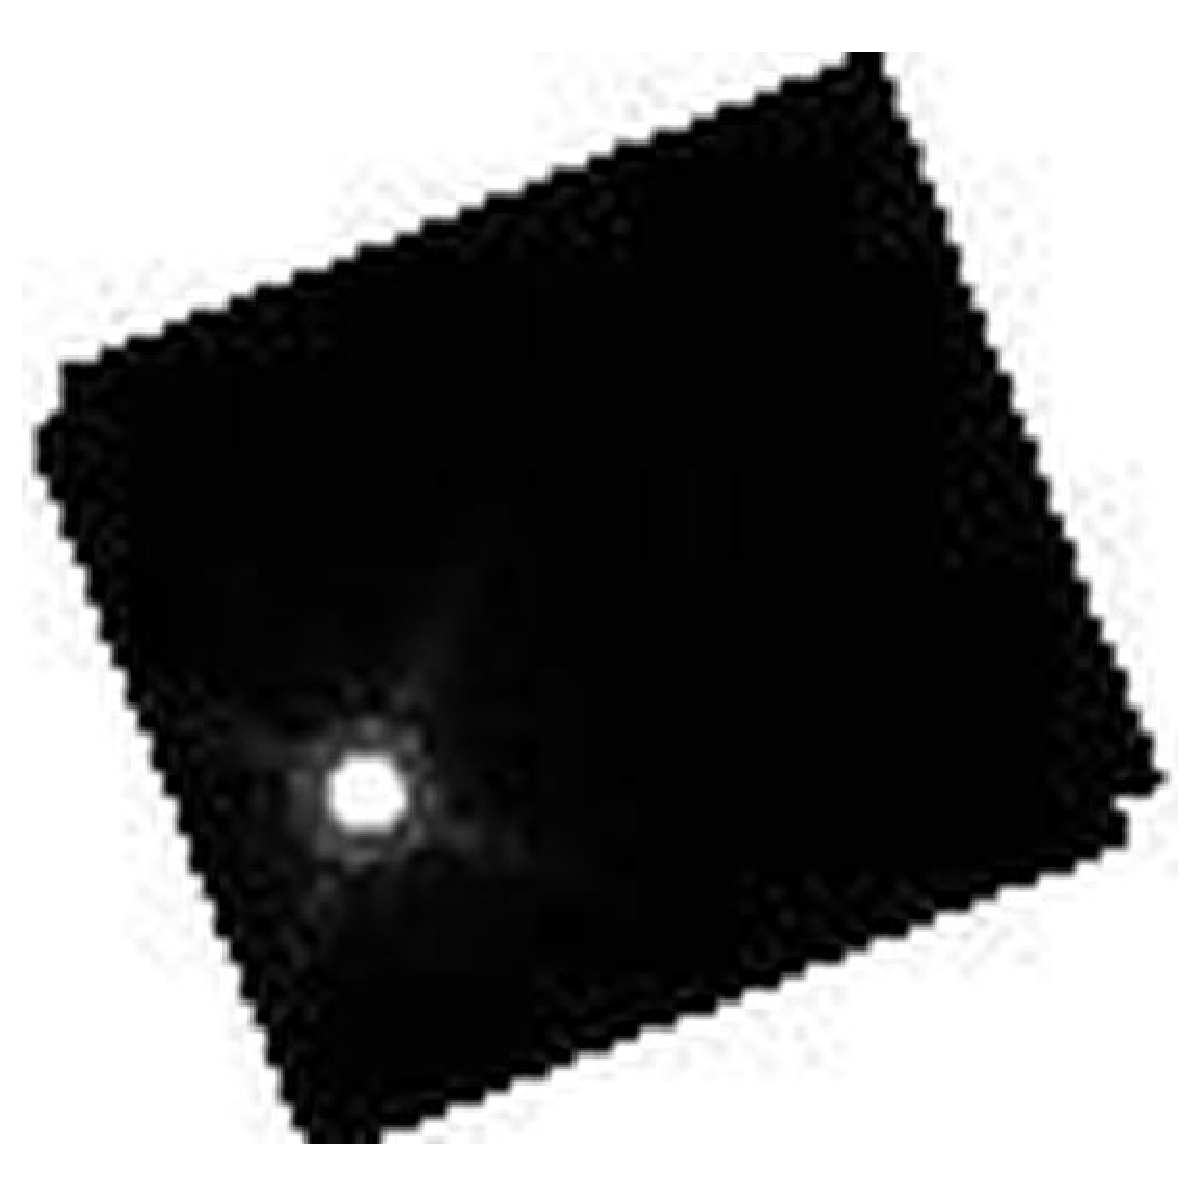
\includegraphics[width=0.18\textwidth]{\thedatafolder/img_tti_base_0_2.pdf} \\ \input{\thedatafolder/propid_tti_base_0_2.txt} & \centering 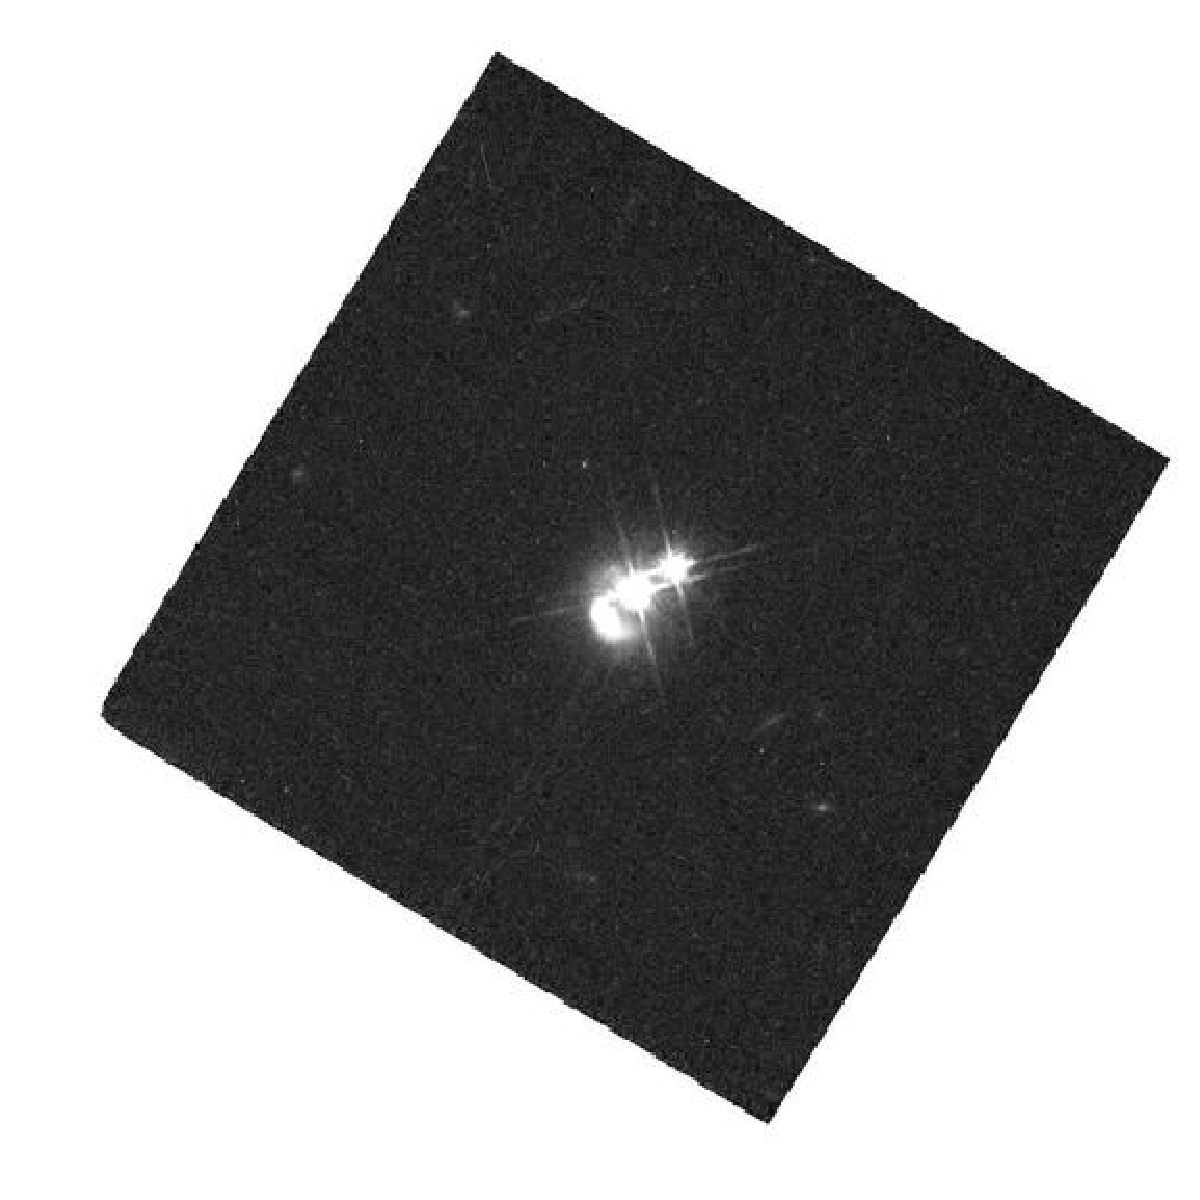
\includegraphics[width=0.18\textwidth]{\thedatafolder/img_tti_base_0_3.pdf} \\ \input{\thedatafolder/propid_tti_base_0_3.txt}  \tabularnewline
      \midrule
      \texttt{\input{\thedatafolder/query_tti_base_2.txt}} \vspace{20mm} & \centering 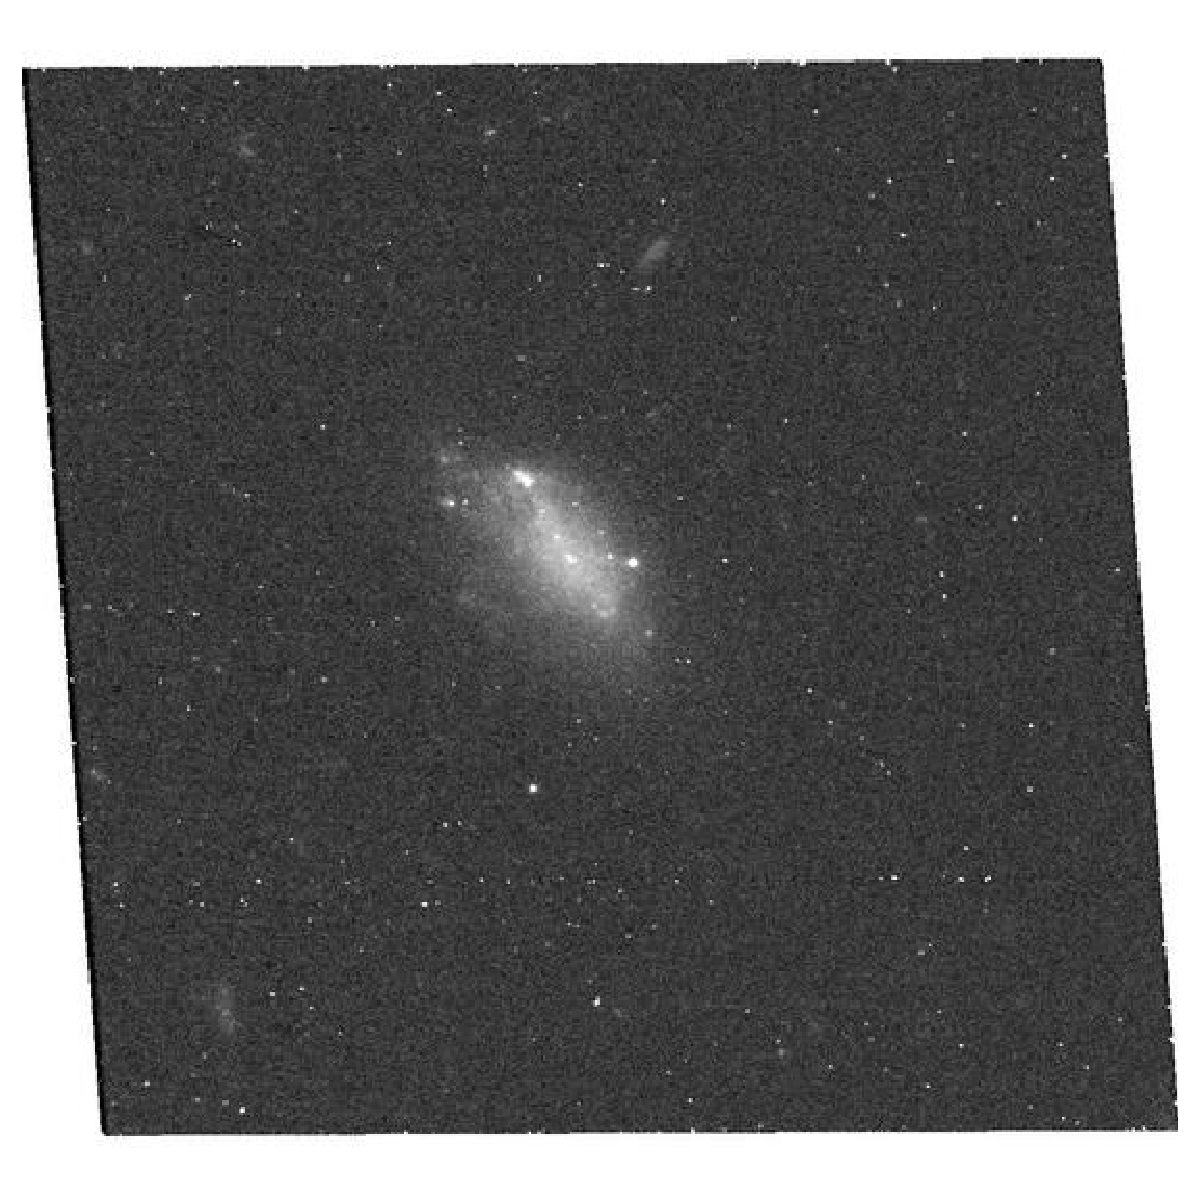
\includegraphics[width=0.18\textwidth]{\thedatafolder/img_tti_base_2_0.pdf} \\ \input{\thedatafolder/propid_tti_base_2_0.txt} & \centering 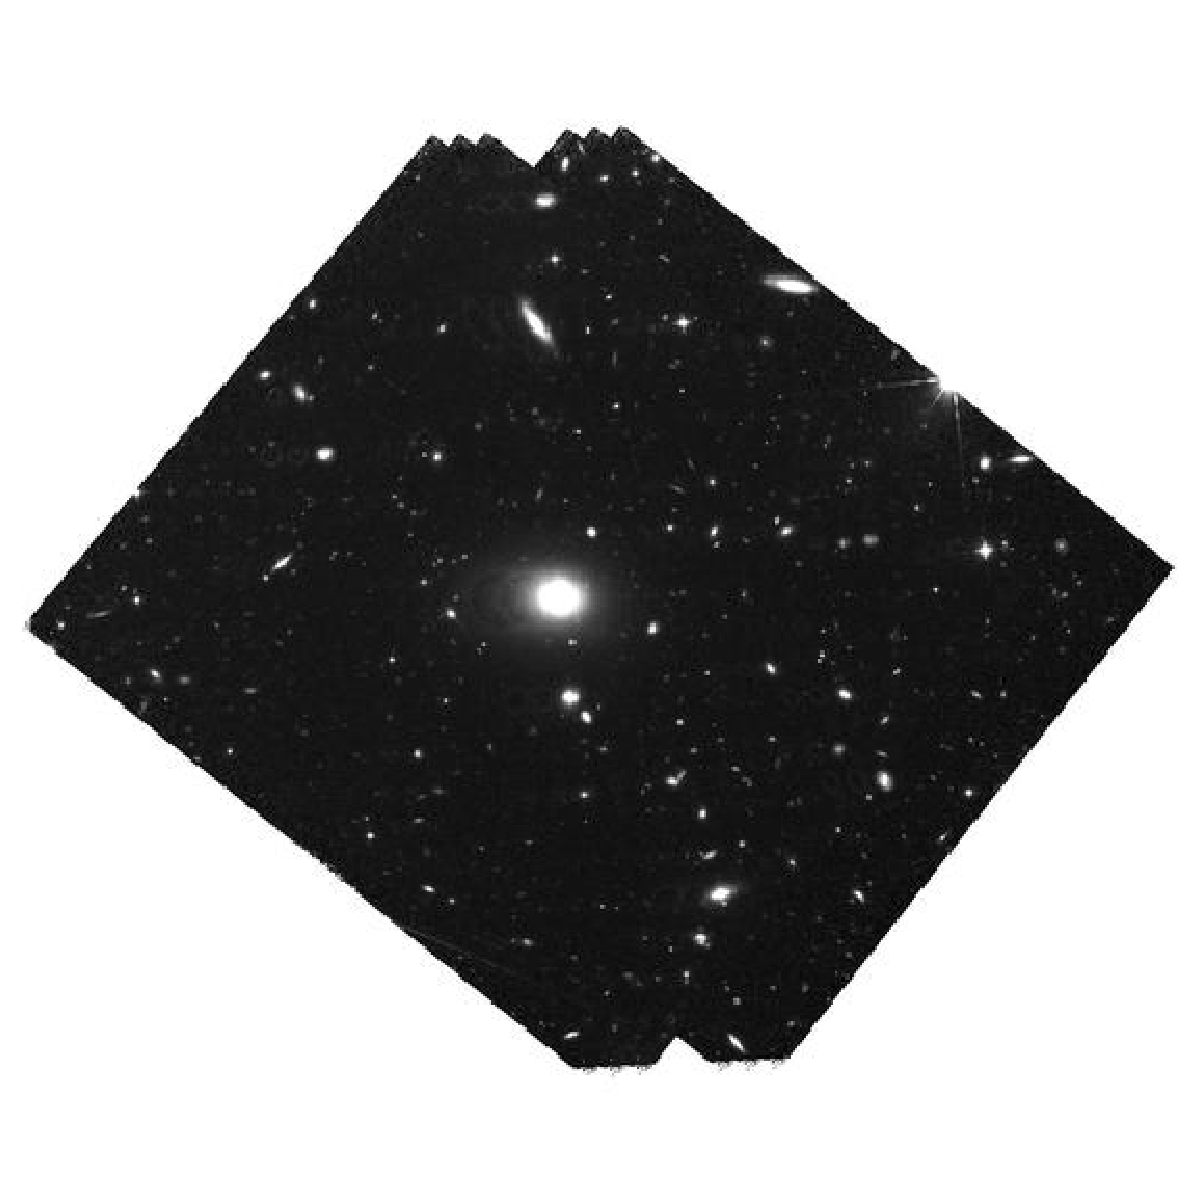
\includegraphics[width=0.18\textwidth]{\thedatafolder/img_tti_base_2_1.pdf} \\ \input{\thedatafolder/propid_tti_base_2_1.txt} & \centering 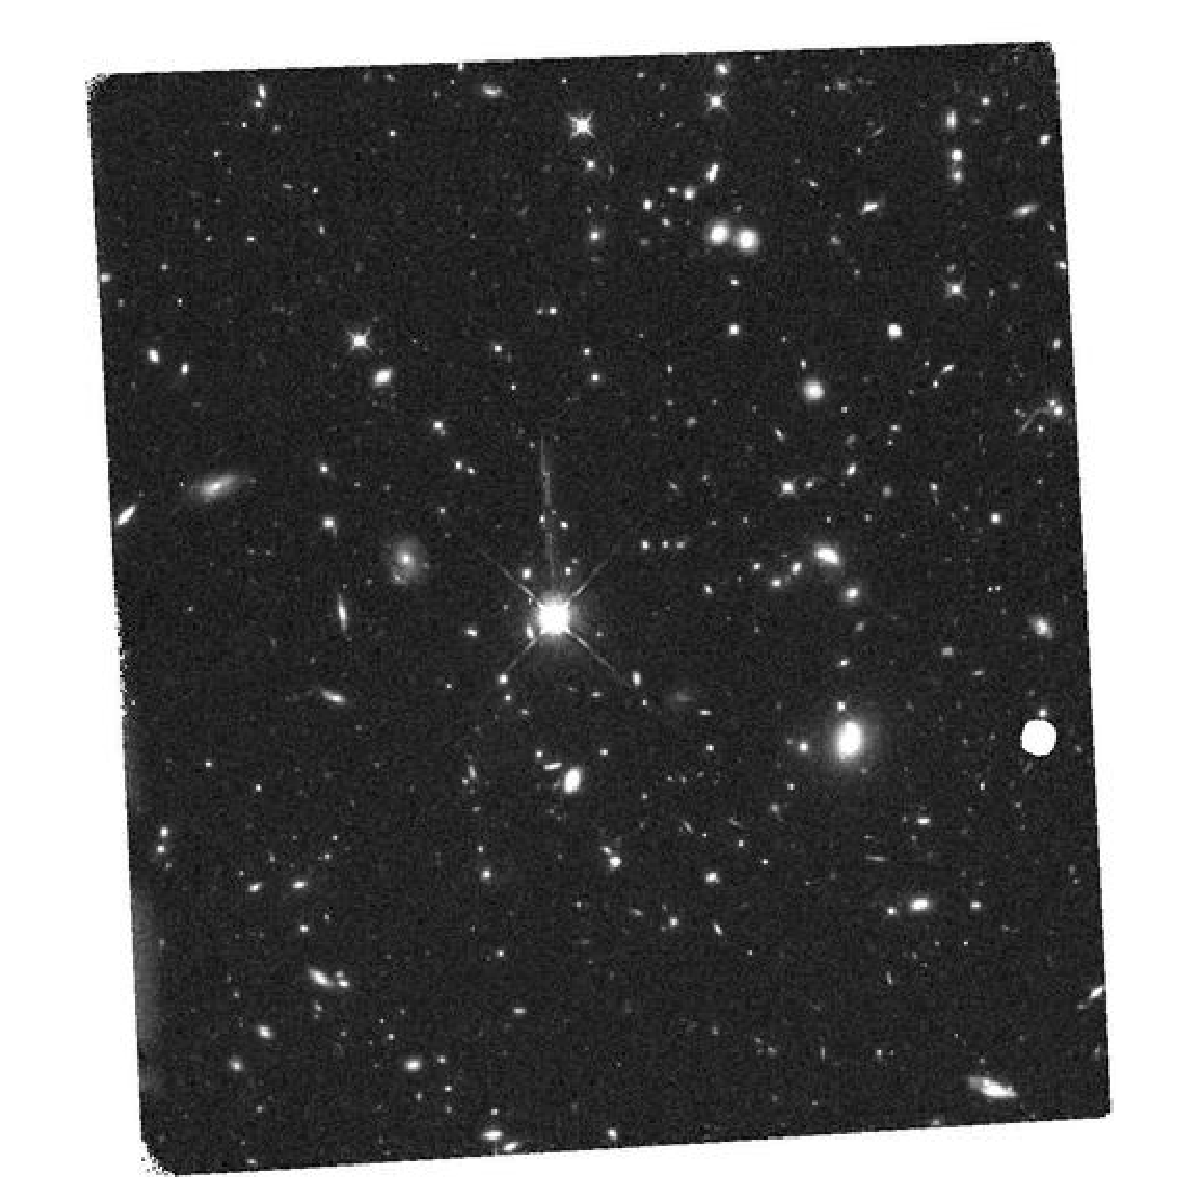
\includegraphics[width=0.18\textwidth]{\thedatafolder/img_tti_base_2_2.pdf} \\ \input{\thedatafolder/propid_tti_base_2_2.txt} & \centering 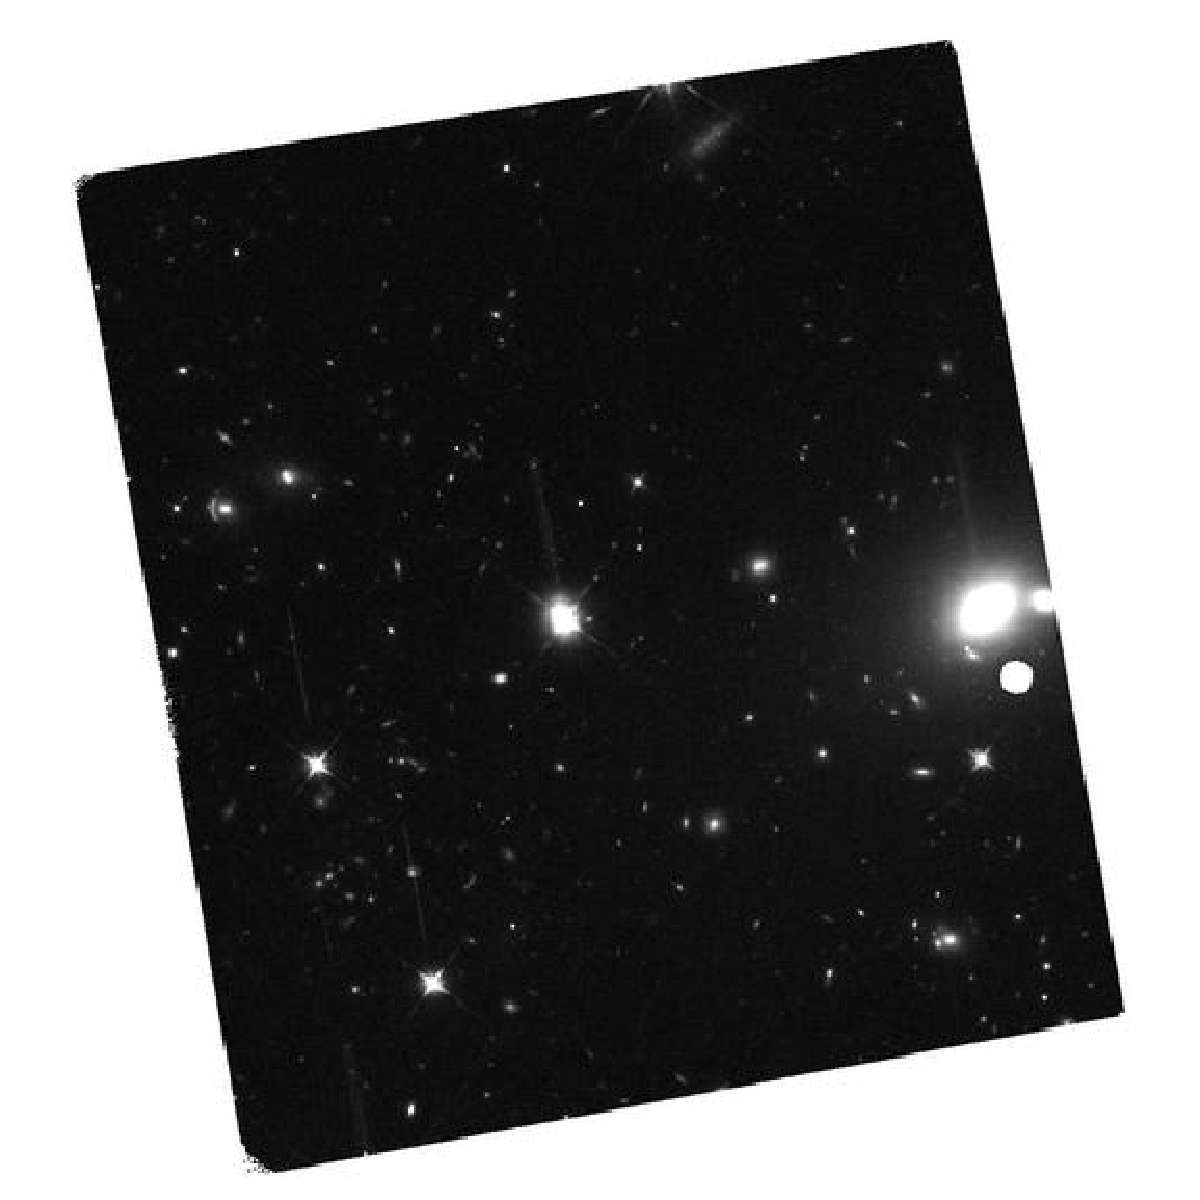
\includegraphics[width=0.18\textwidth]{\thedatafolder/img_tti_base_2_3.pdf} \\ \input{\thedatafolder/propid_tti_base_2_3.txt}  \tabularnewline
      \midrule
      \texttt{\input{\thedatafolder/query_tti_base_3.txt}} \vspace{20mm} & \centering 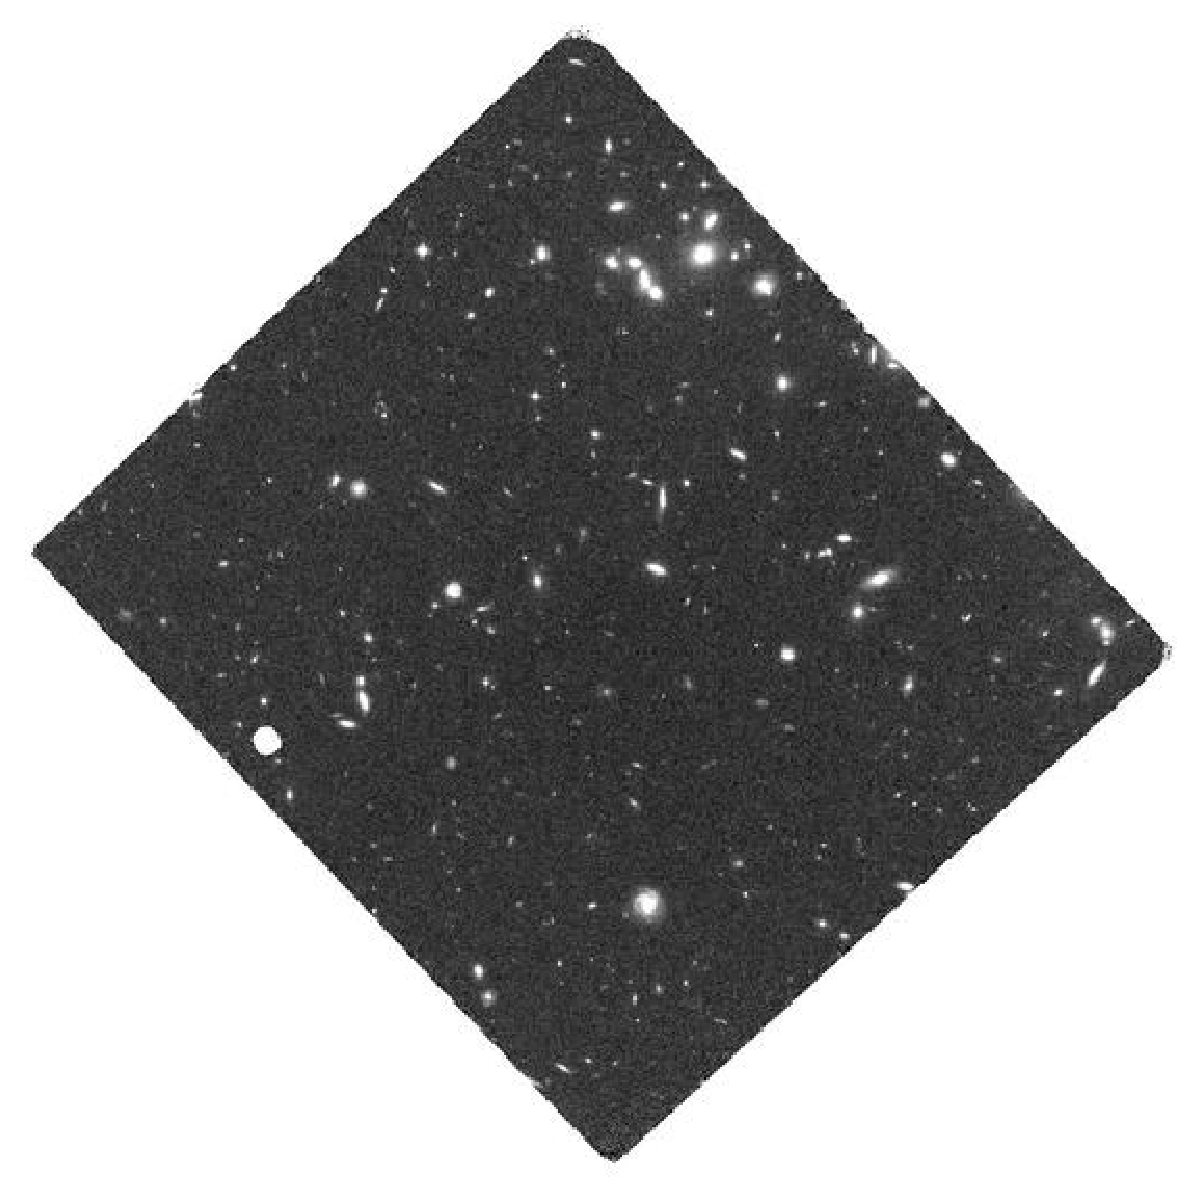
\includegraphics[width=0.18\textwidth]{\thedatafolder/img_tti_base_3_0.pdf} \\ \input{\thedatafolder/propid_tti_base_3_0.txt} & \centering 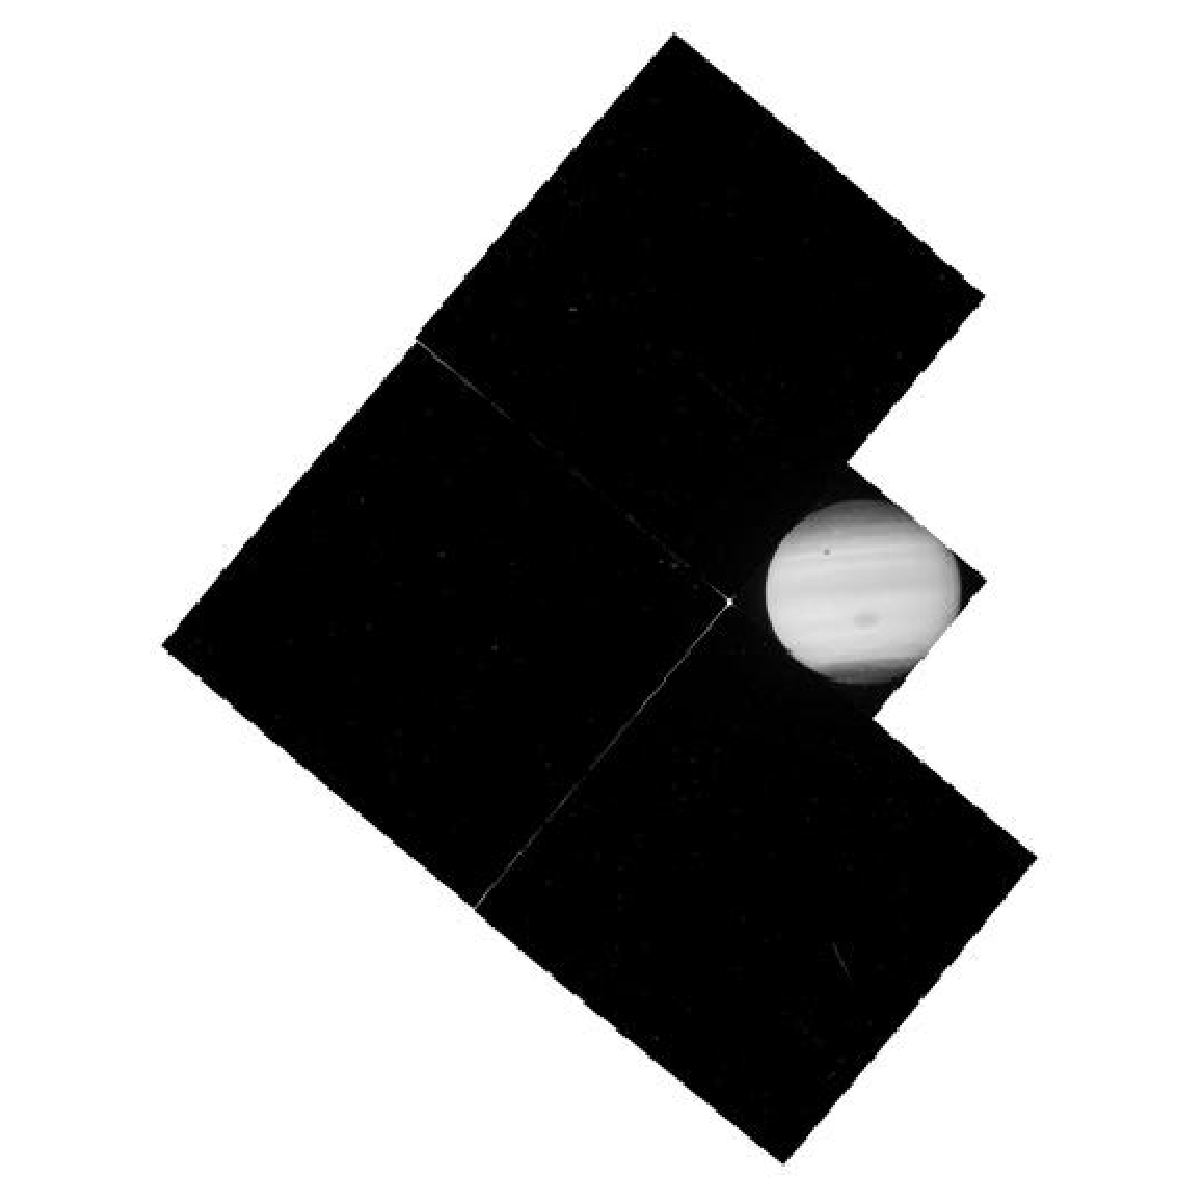
\includegraphics[width=0.18\textwidth]{\thedatafolder/img_tti_base_3_1.pdf} \\ \input{\thedatafolder/propid_tti_base_3_1.txt} & \centering 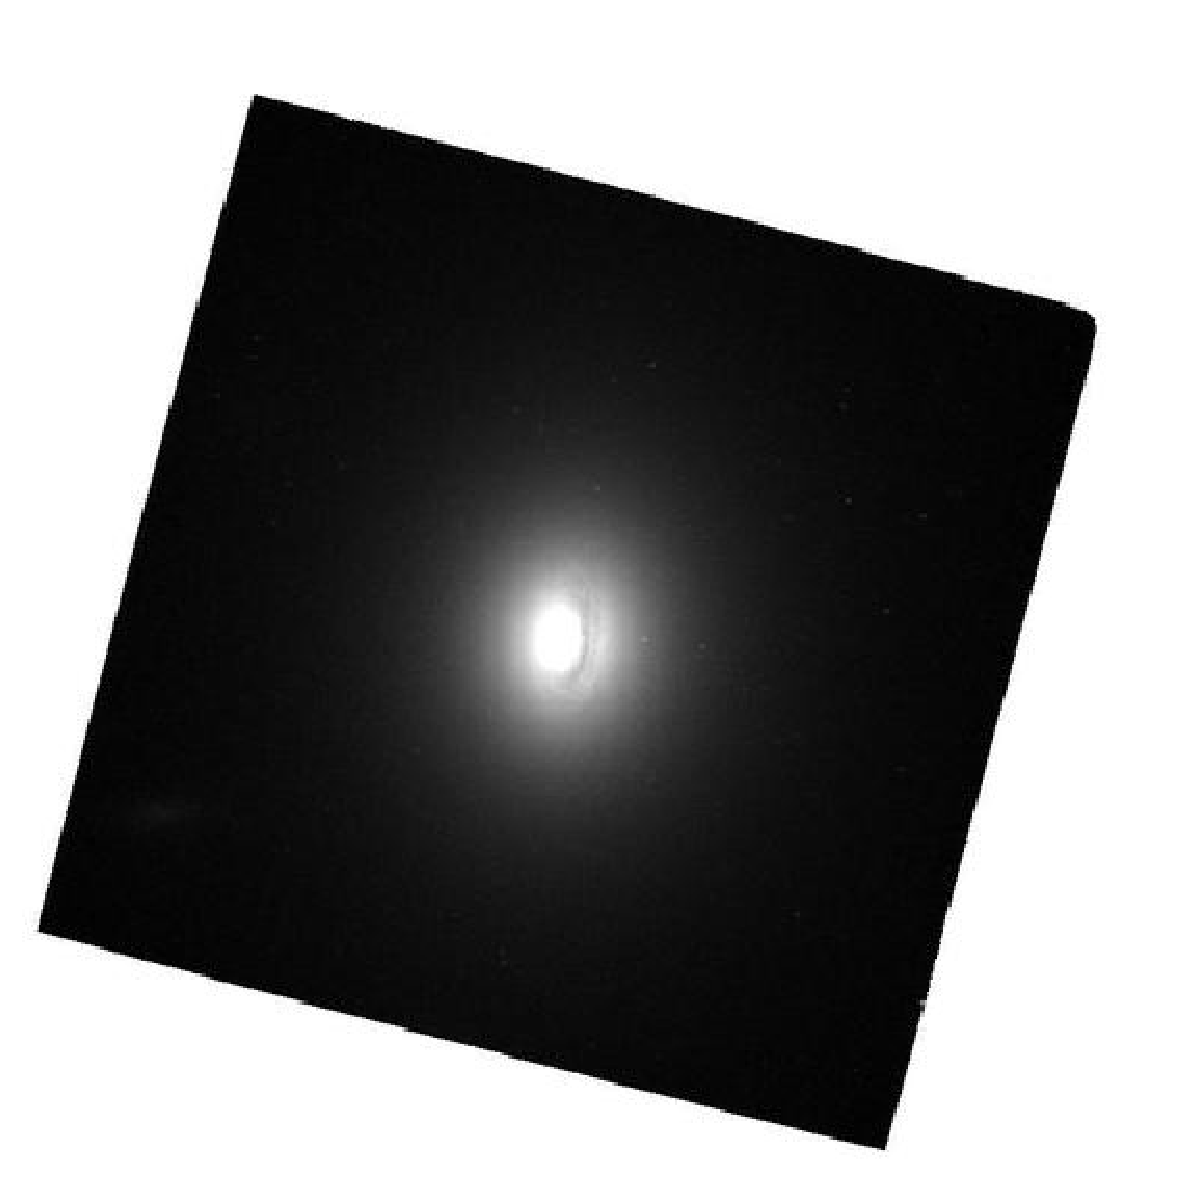
\includegraphics[width=0.18\textwidth]{\thedatafolder/img_tti_base_3_2.pdf} \\ \input{\thedatafolder/propid_tti_base_3_2.txt} & \centering 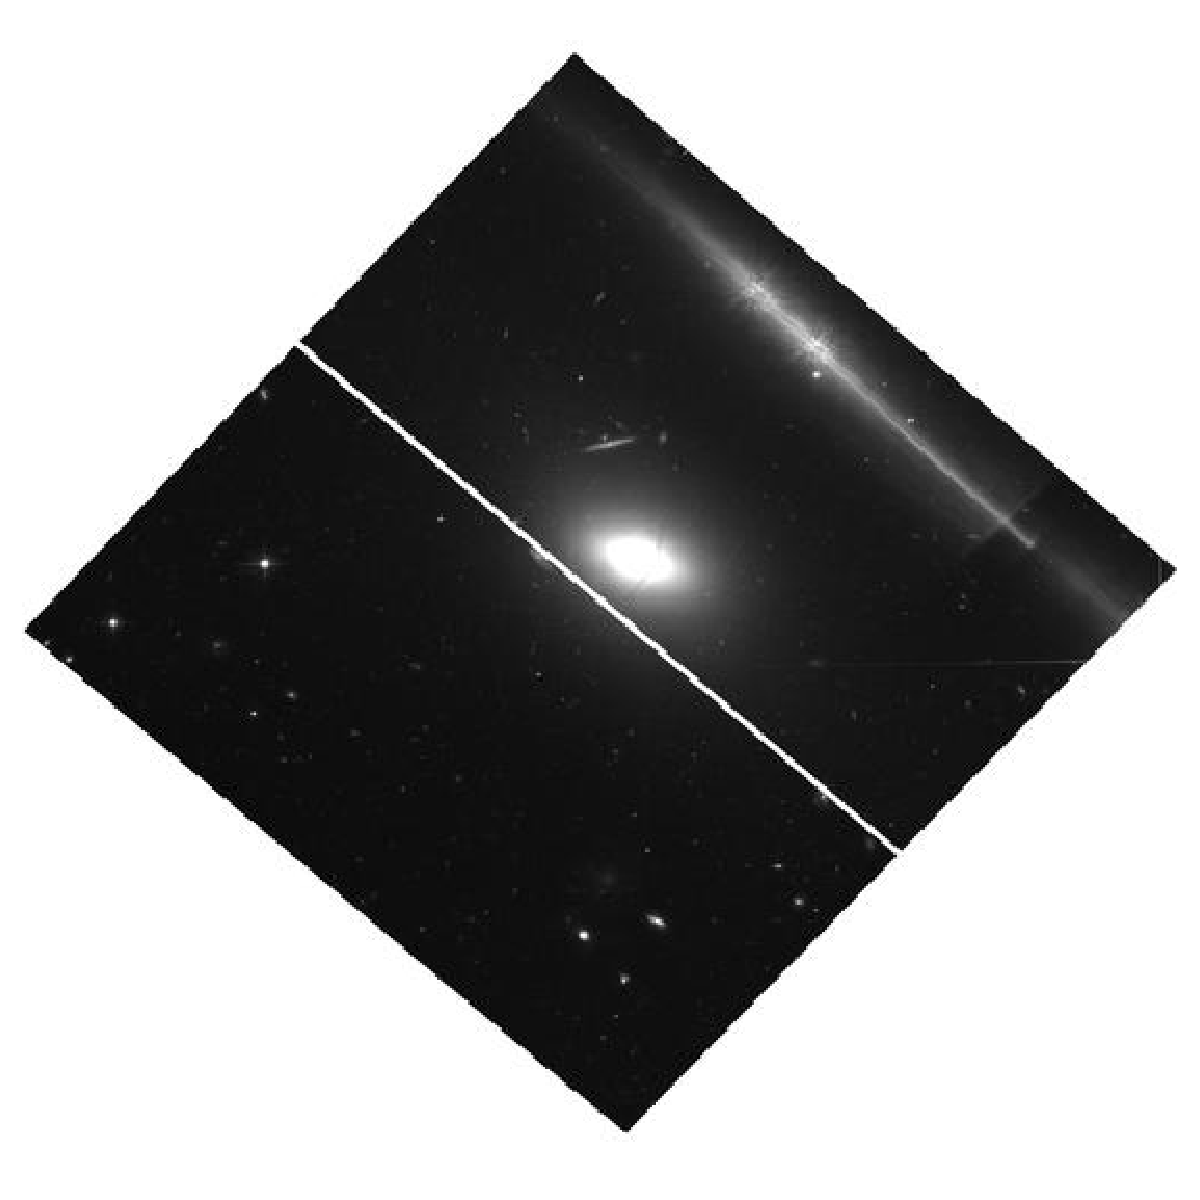
\includegraphics[width=0.18\textwidth]{\thedatafolder/img_tti_base_3_3.pdf} \\ \input{\thedatafolder/propid_tti_base_3_3.txt}  \tabularnewline
      \bottomrule
  \end{tabular}
  \caption{For four text queries (left-most column), the four most similar images from the validation dataset by cosine similarity when using the \textbf{\textcolor{deeppurple}{base CLIP model}} (CLIP-ViT-B/16). The proposal ID associated with each image is given below the image and contains a hyperlink to the MAST page corresponding to the proposal.}
  \label{tab:tti_base}
\end{table}

% \begin{figure*}[!h]
% 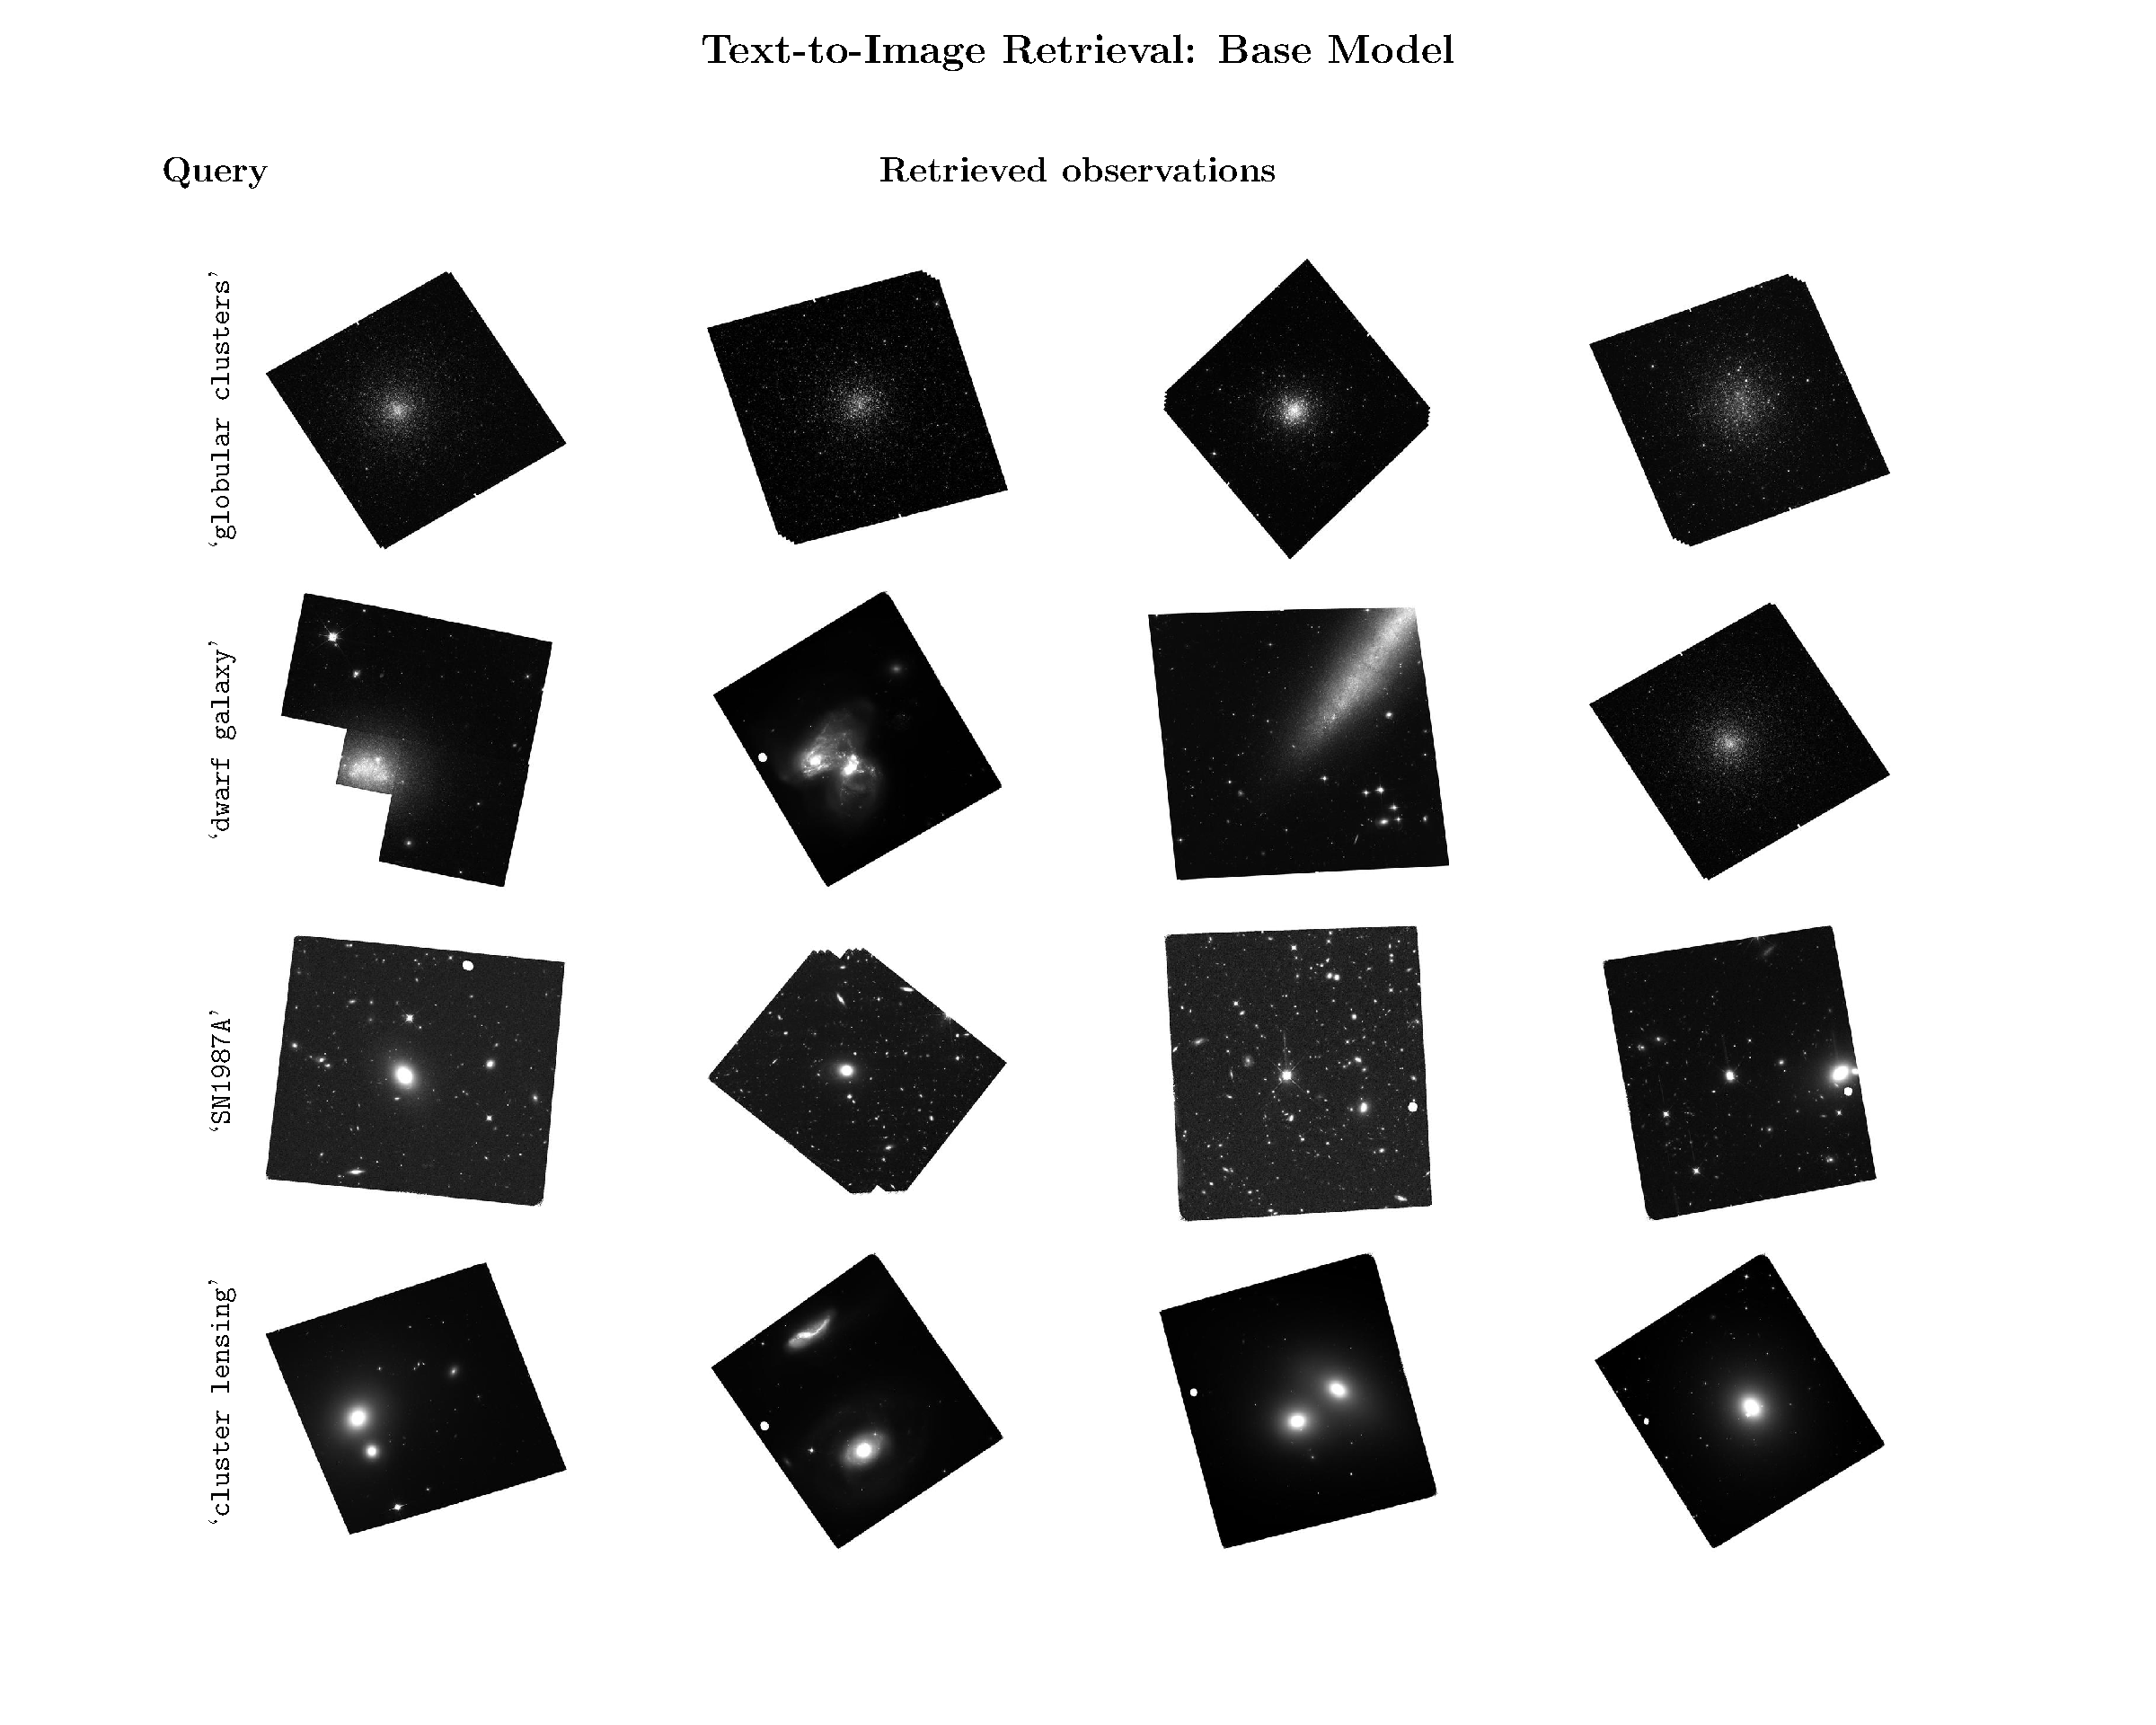
\includegraphics[width=0.95\textwidth]{plots/tti_base.pdf}
% \caption{Image retrieval using the base CLIP model on four curated queries. \SM{Horizontal lines} \SM{Query not rotated} \SM{Same for next Figure.} \SM{Put text ``Base Model'' in consistent colour to legend.} \SM{Say top 4} \SM{Say that for science we care about the distributions of things.}}
% \label{fig:tti_base}
% \end{figure*}

% \begin{figure*}[!h]
% 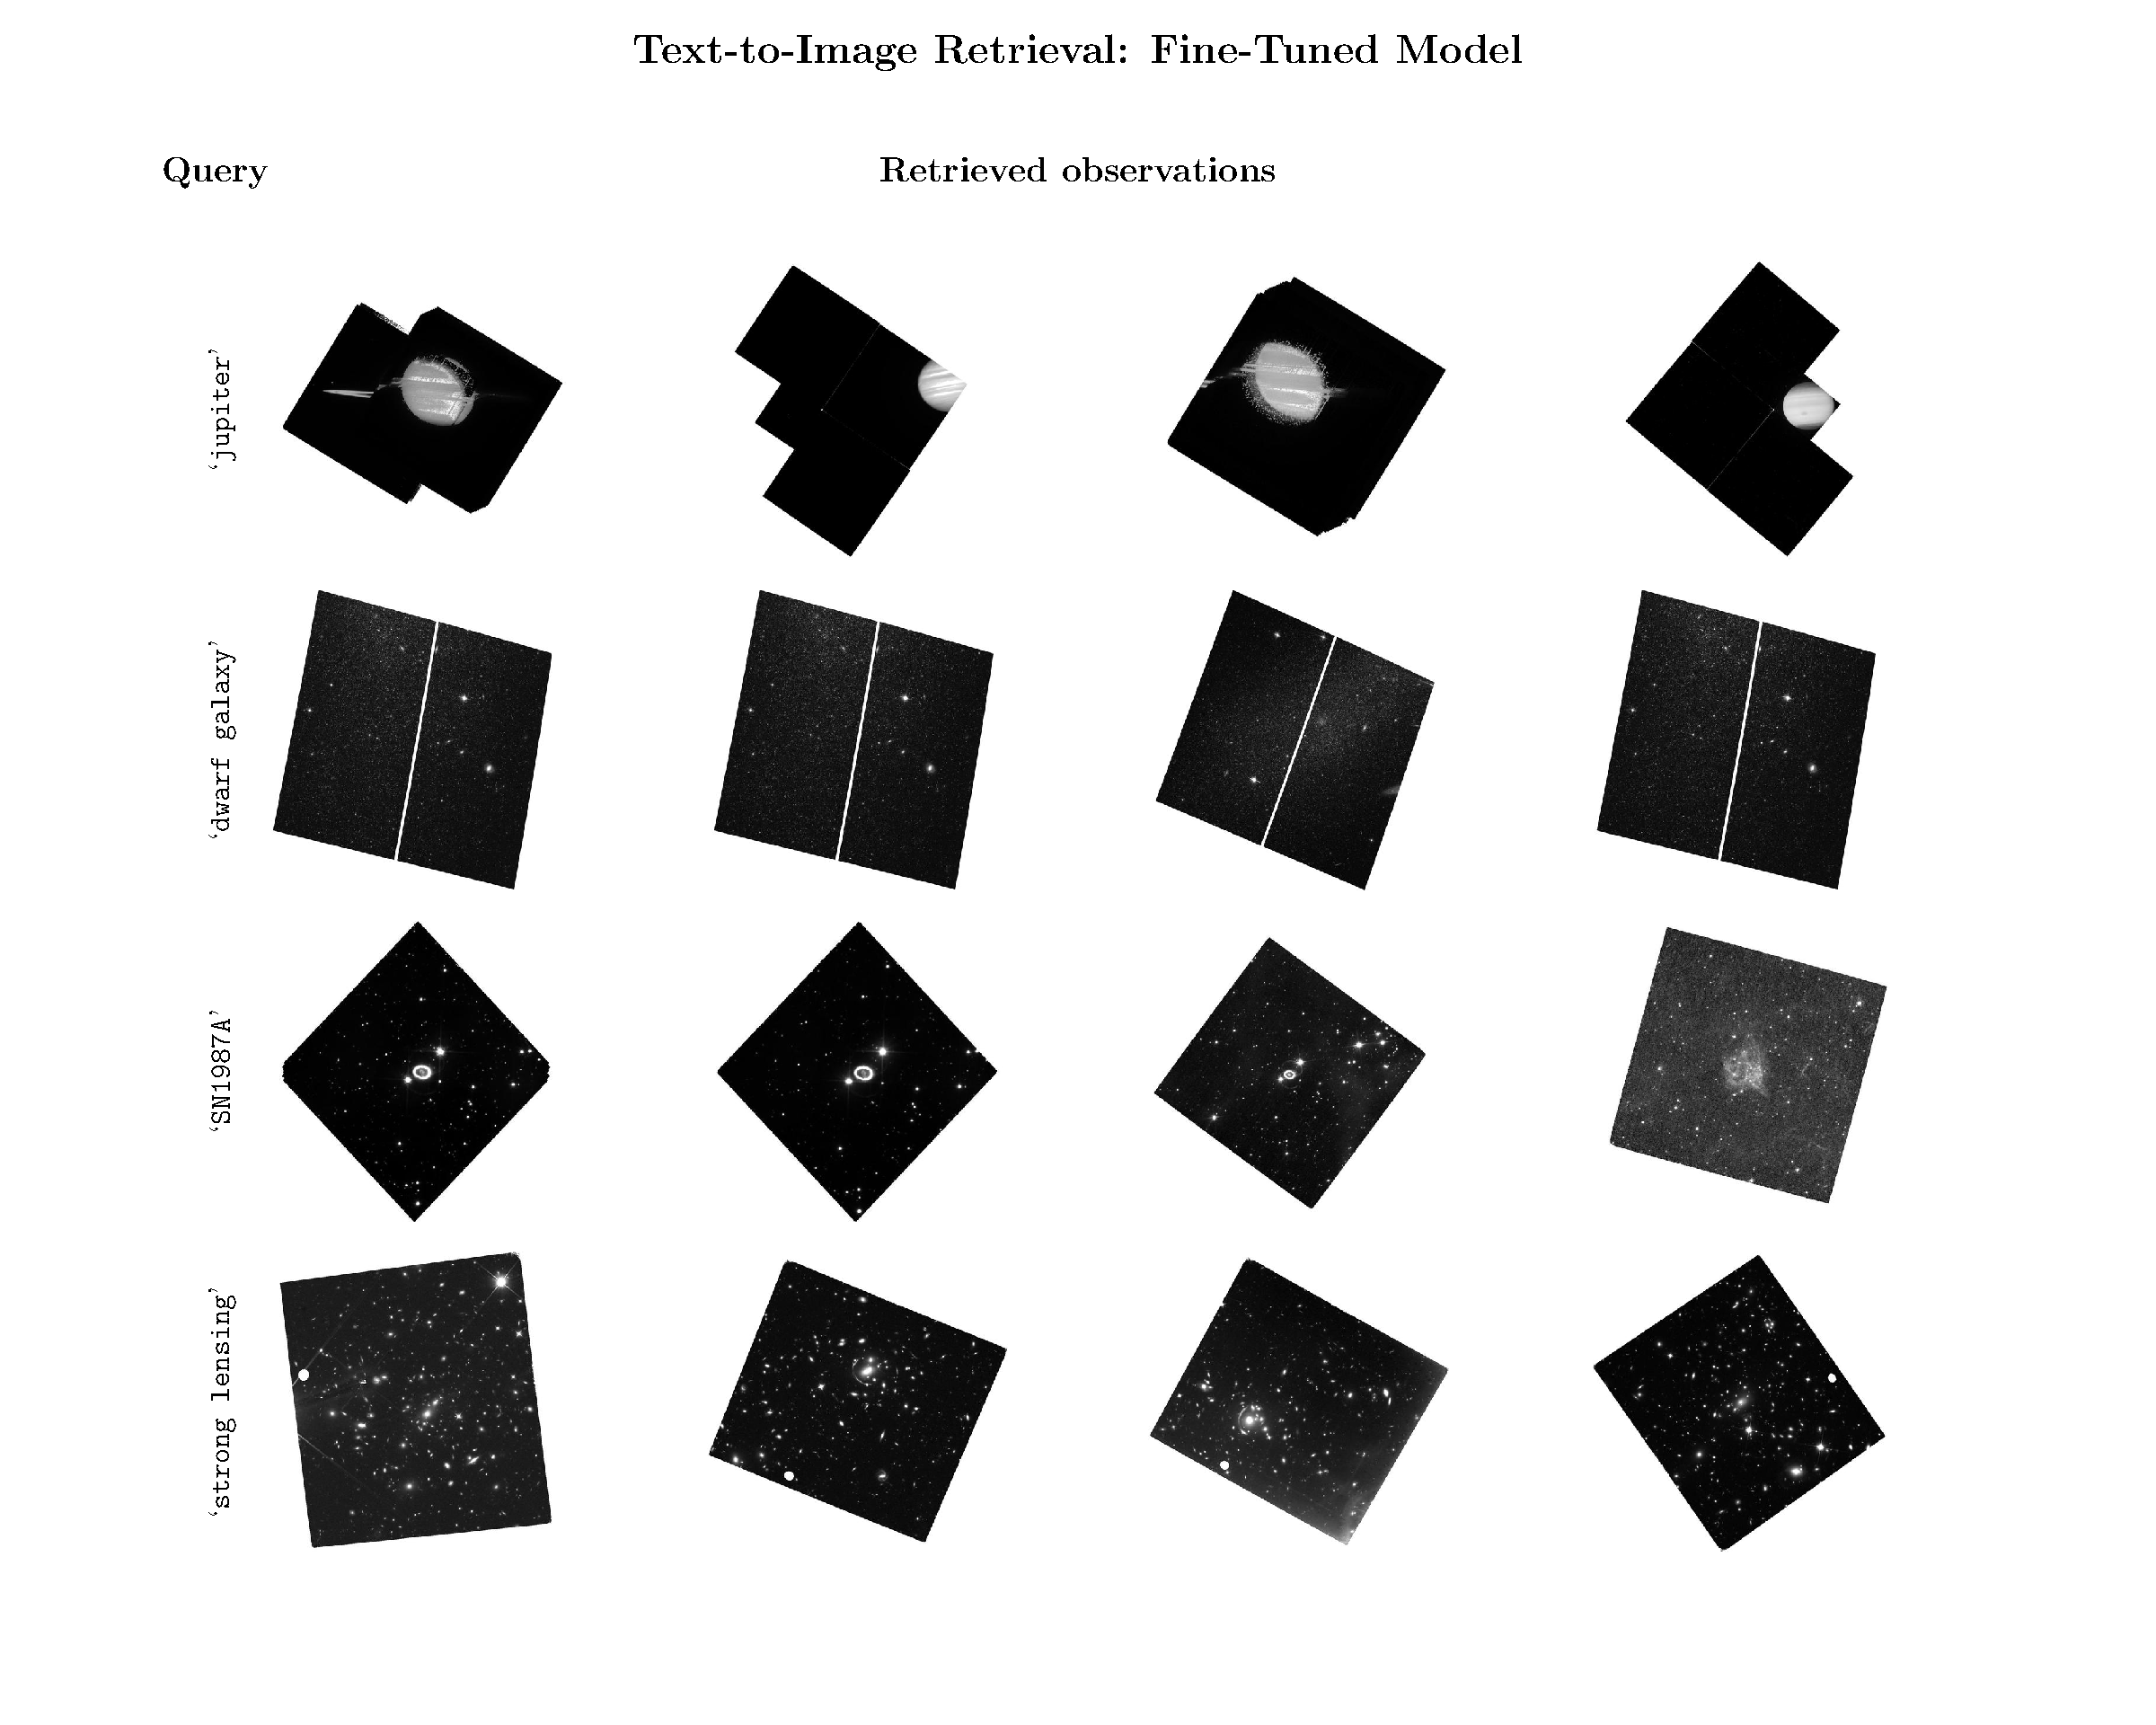
\includegraphics[width=0.95\textwidth]{plots/tti.pdf}
% \caption{Image retrieval using the fine-tuned CLIP model on four curated queries.}
% \label{fig:tti}
% \end{figure*}

\begin{table}[h!]
  \centering
  \begin{tabular}{m{3cm} p{3cm} p{3cm} p{3cm} p{3cm}}
      \toprule
      \centering \bfseries Query & \multicolumn{4}{c}{\bfseries{Top-4 most similar images using \textcolor{deepred}{summary fine-tuned CLIP model}}} \tabularnewline
      \midrule
      \texttt{\input{\thedatafolder/query_tti_1.txt}} \vspace{20mm} & \centering 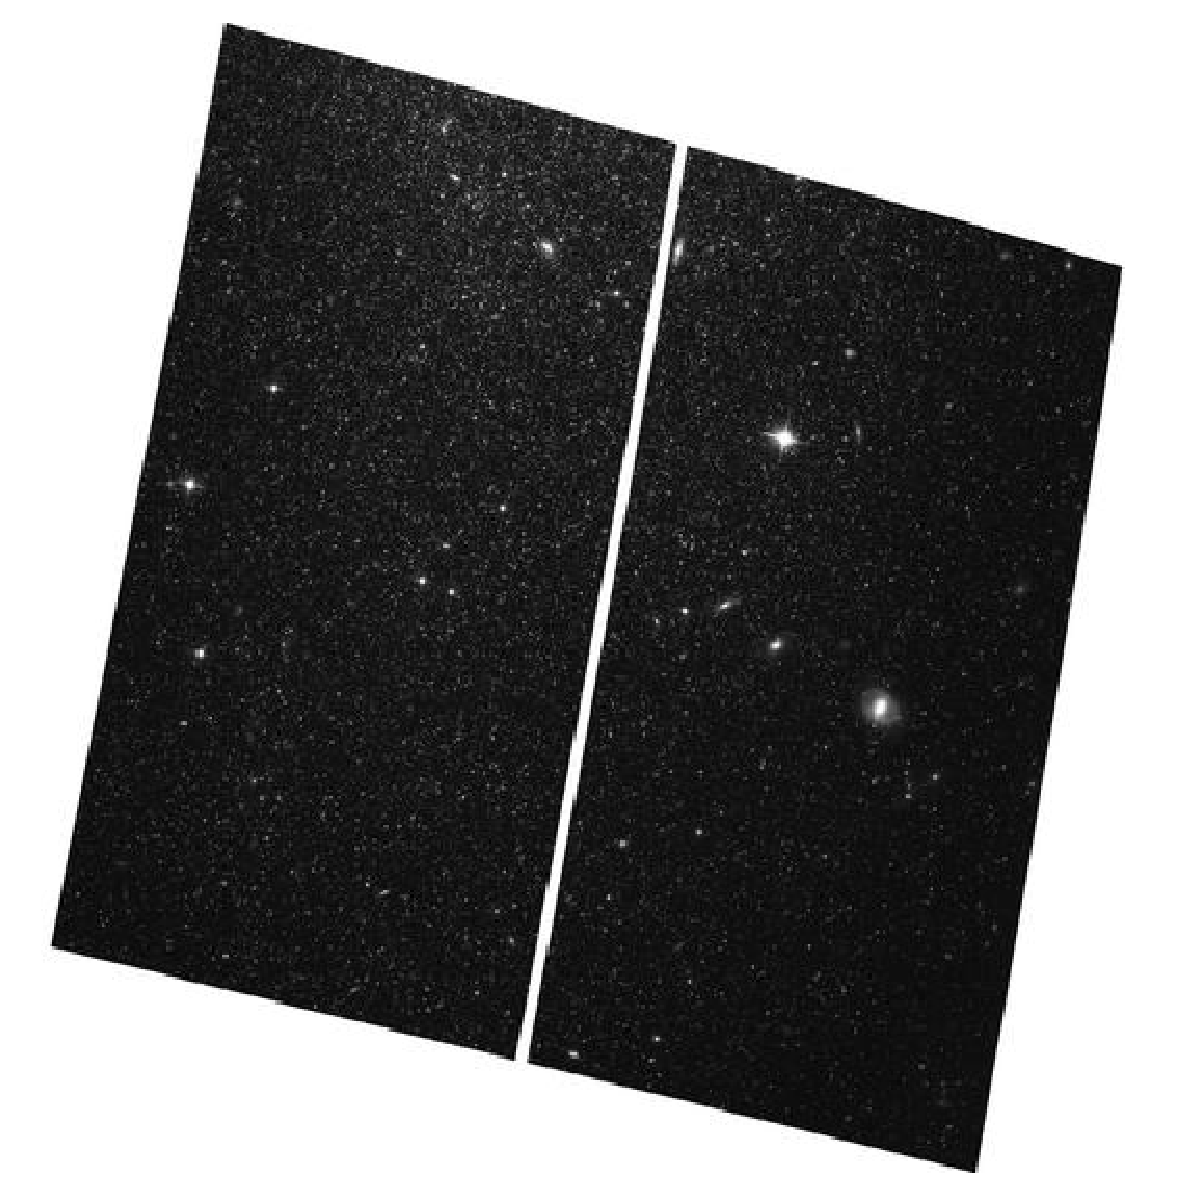
\includegraphics[width=0.18\textwidth]{\thedatafolder/img_tti_1_0.pdf} \\ \input{\thedatafolder/propid_tti_1_0.txt} & \centering 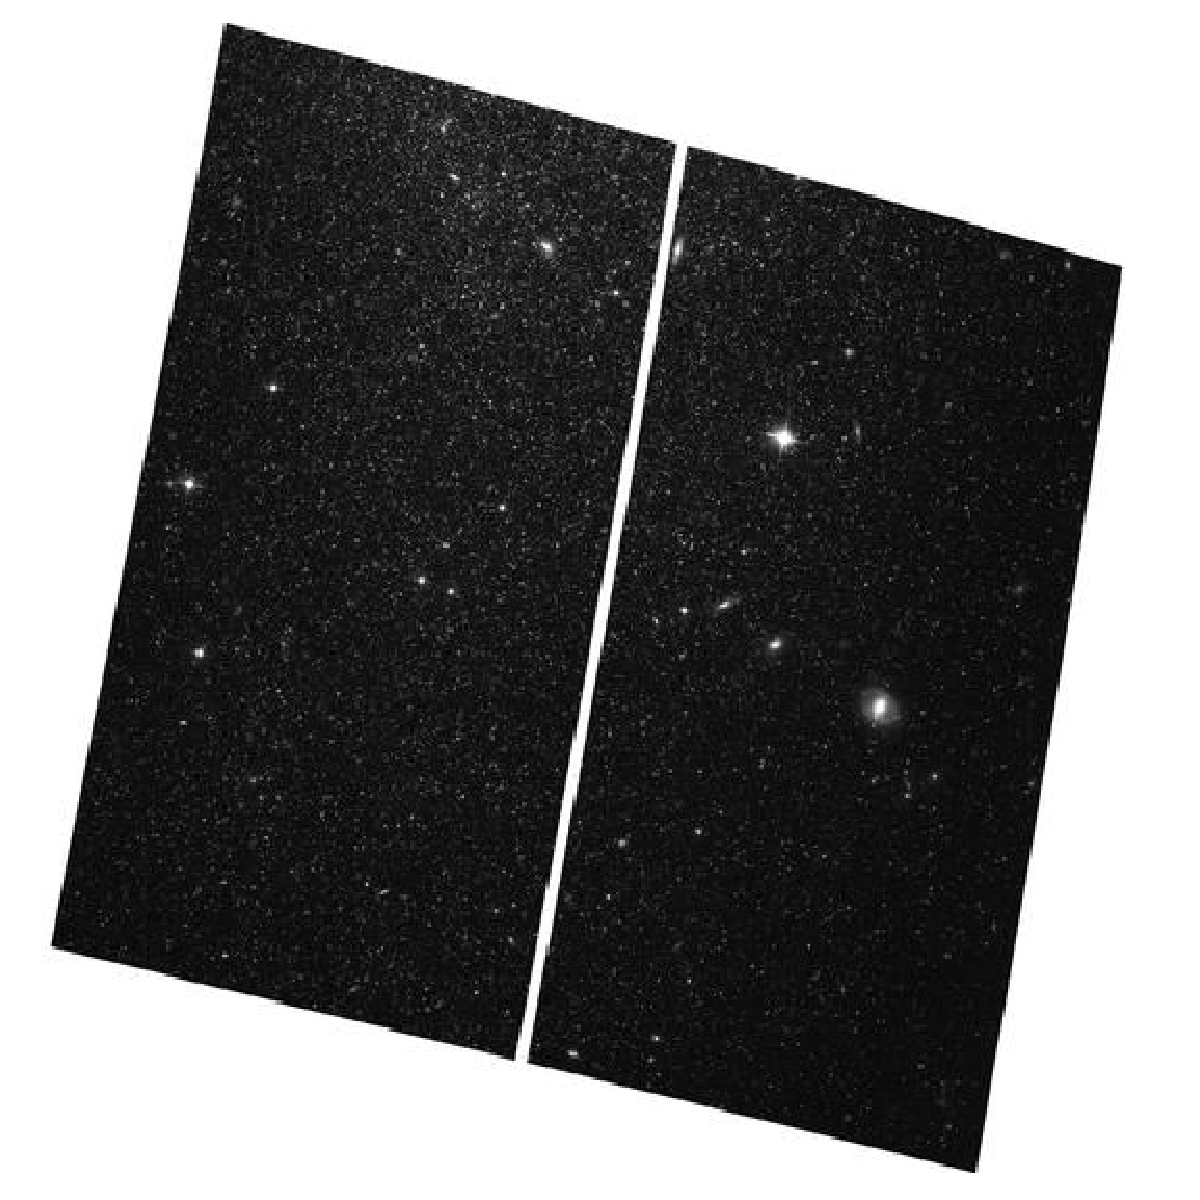
\includegraphics[width=0.18\textwidth]{\thedatafolder/img_tti_1_1.pdf} \\ \input{\thedatafolder/propid_tti_1_1.txt} & \centering 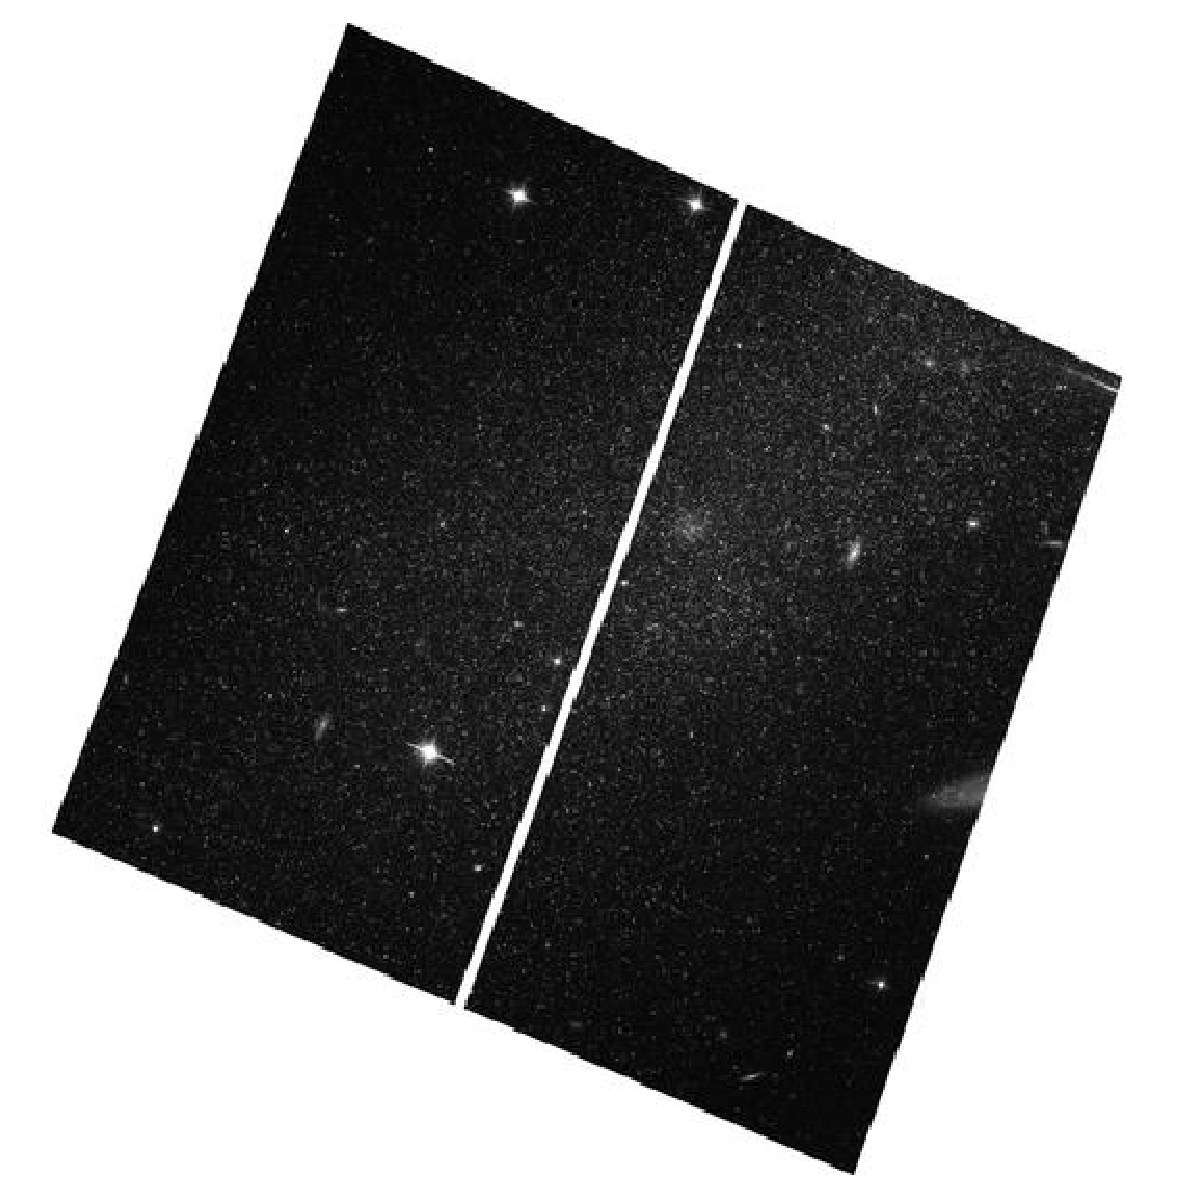
\includegraphics[width=0.18\textwidth]{\thedatafolder/img_tti_1_2.pdf} \\ \input{\thedatafolder/propid_tti_1_2.txt} & \centering 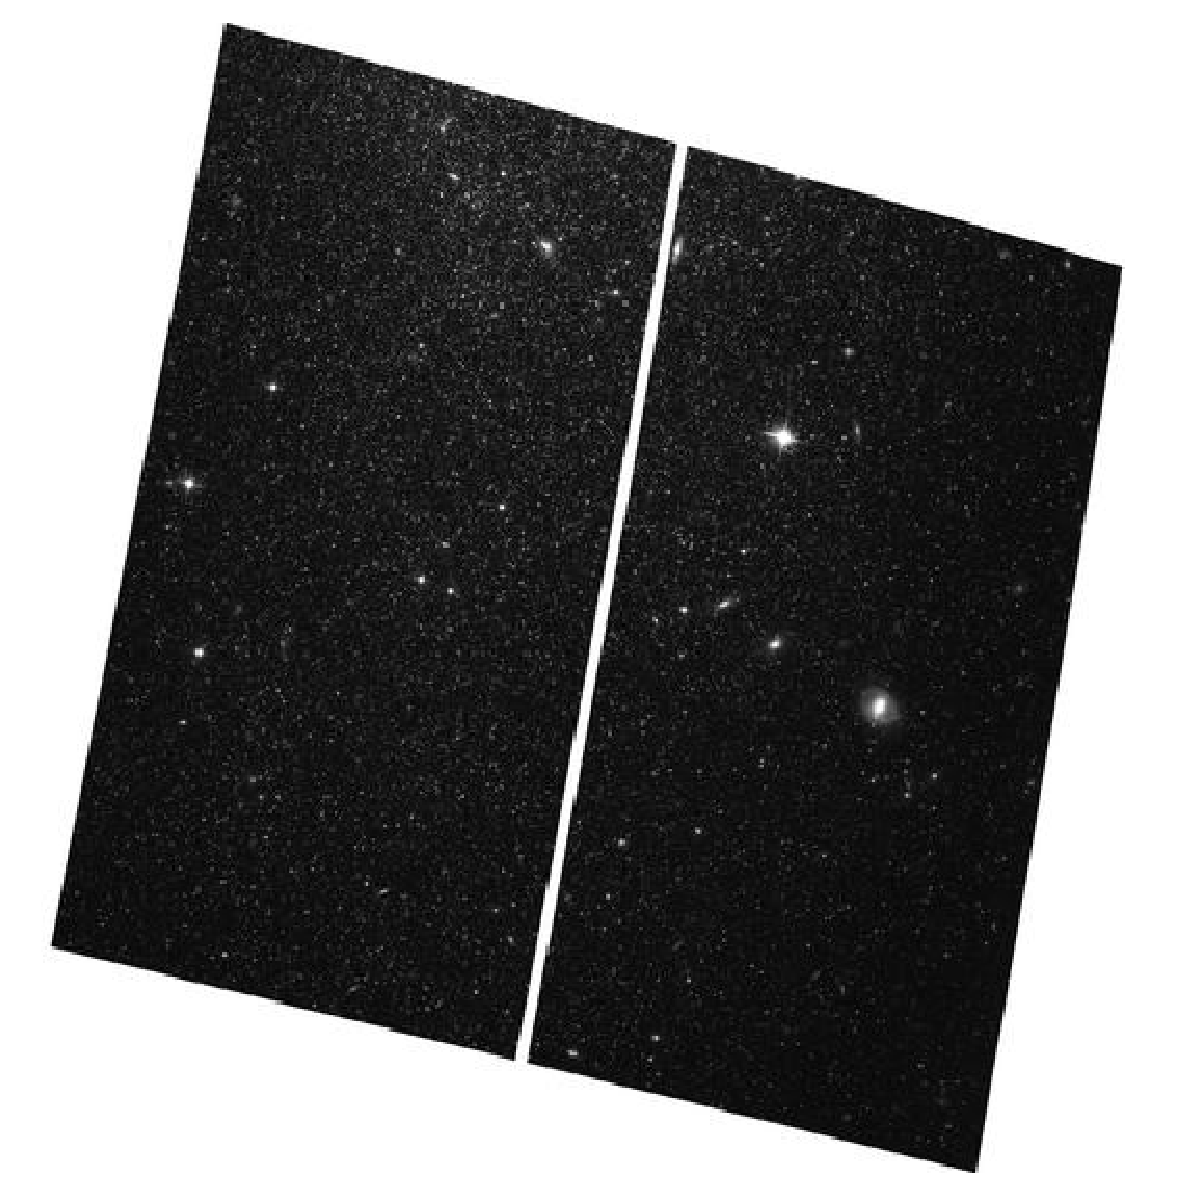
\includegraphics[width=0.18\textwidth]{\thedatafolder/img_tti_1_3.pdf} \\ \input{\thedatafolder/propid_tti_1_3.txt}  \tabularnewline
      \midrule
       \texttt{\input{\thedatafolder/query_tti_0.txt}} \vspace{20mm} & \centering 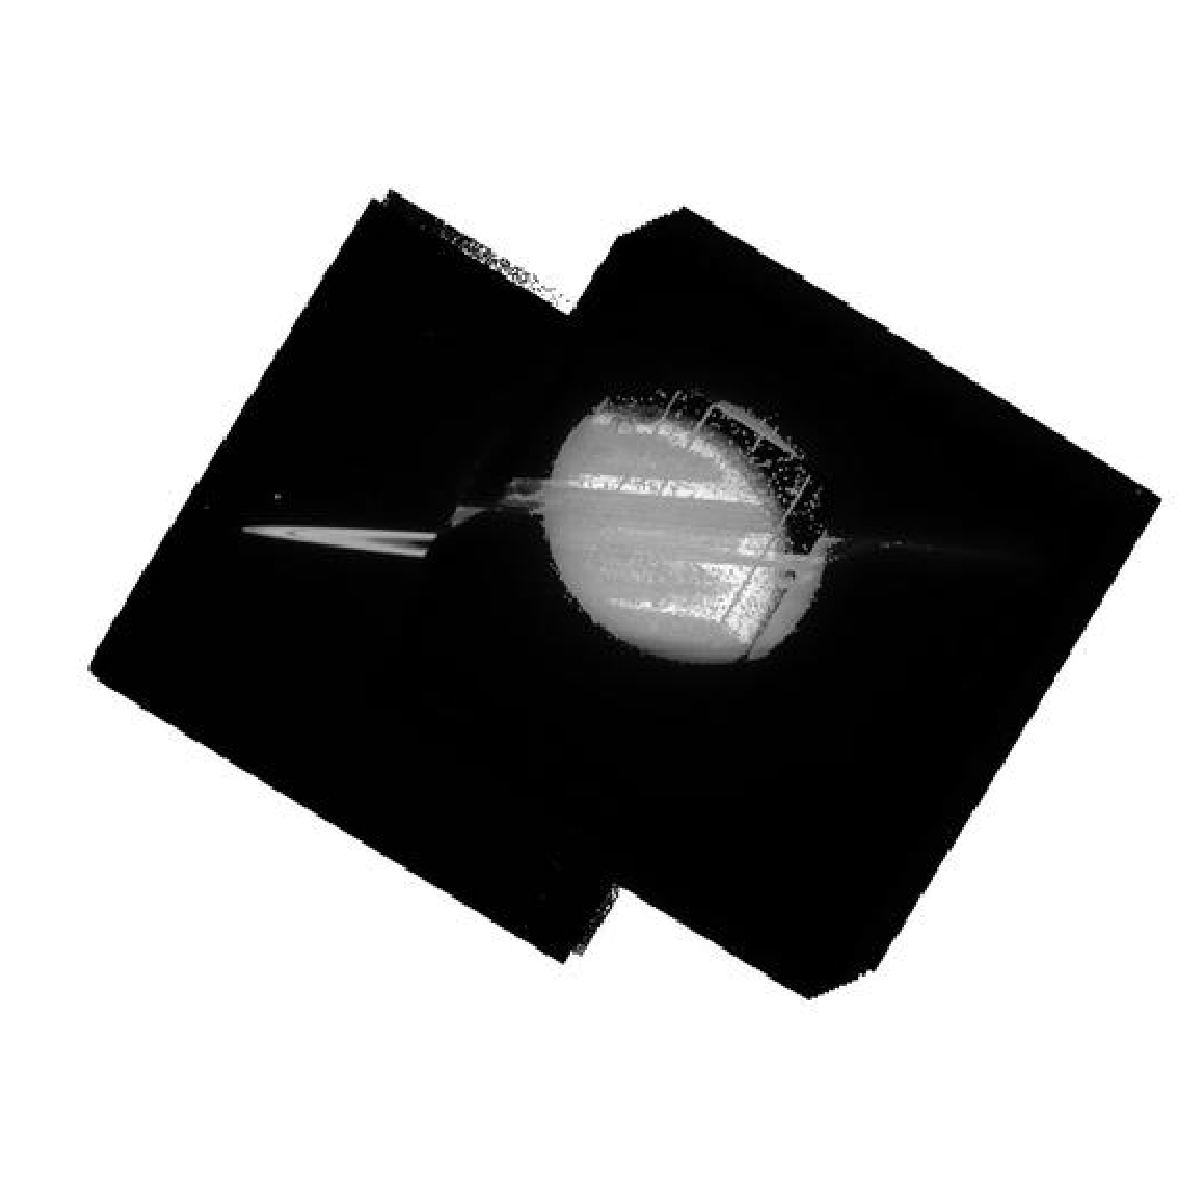
\includegraphics[width=0.18\textwidth]{\thedatafolder/img_tti_0_0.pdf} \\ \input{\thedatafolder/propid_tti_0_0.txt} & \centering 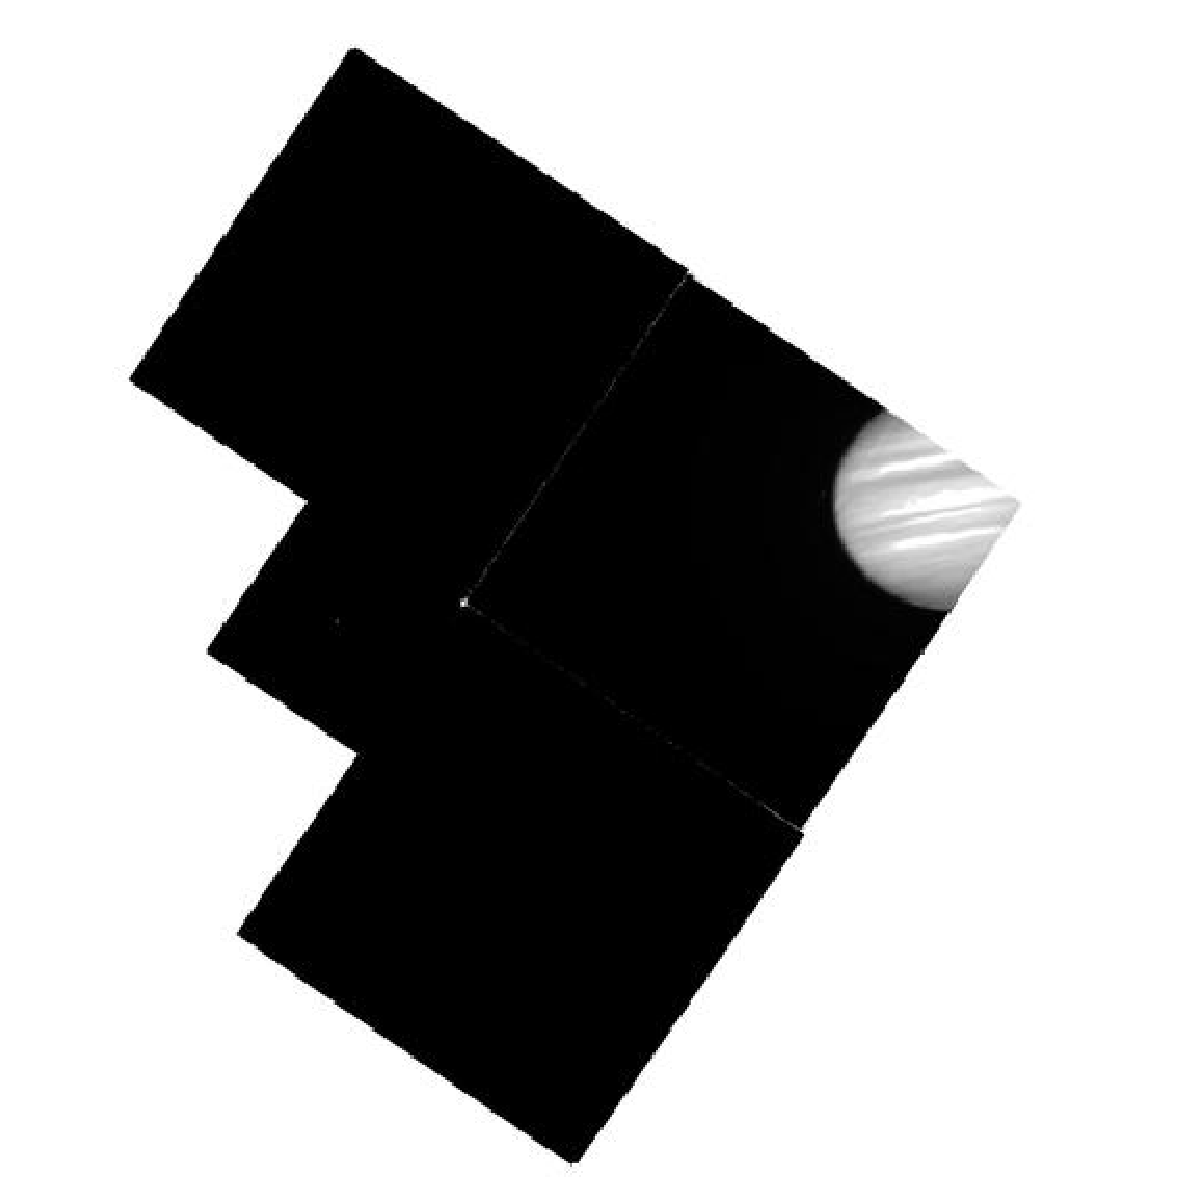
\includegraphics[width=0.18\textwidth]{\thedatafolder/img_tti_0_1.pdf} \\ \input{\thedatafolder/propid_tti_0_1.txt} & \centering 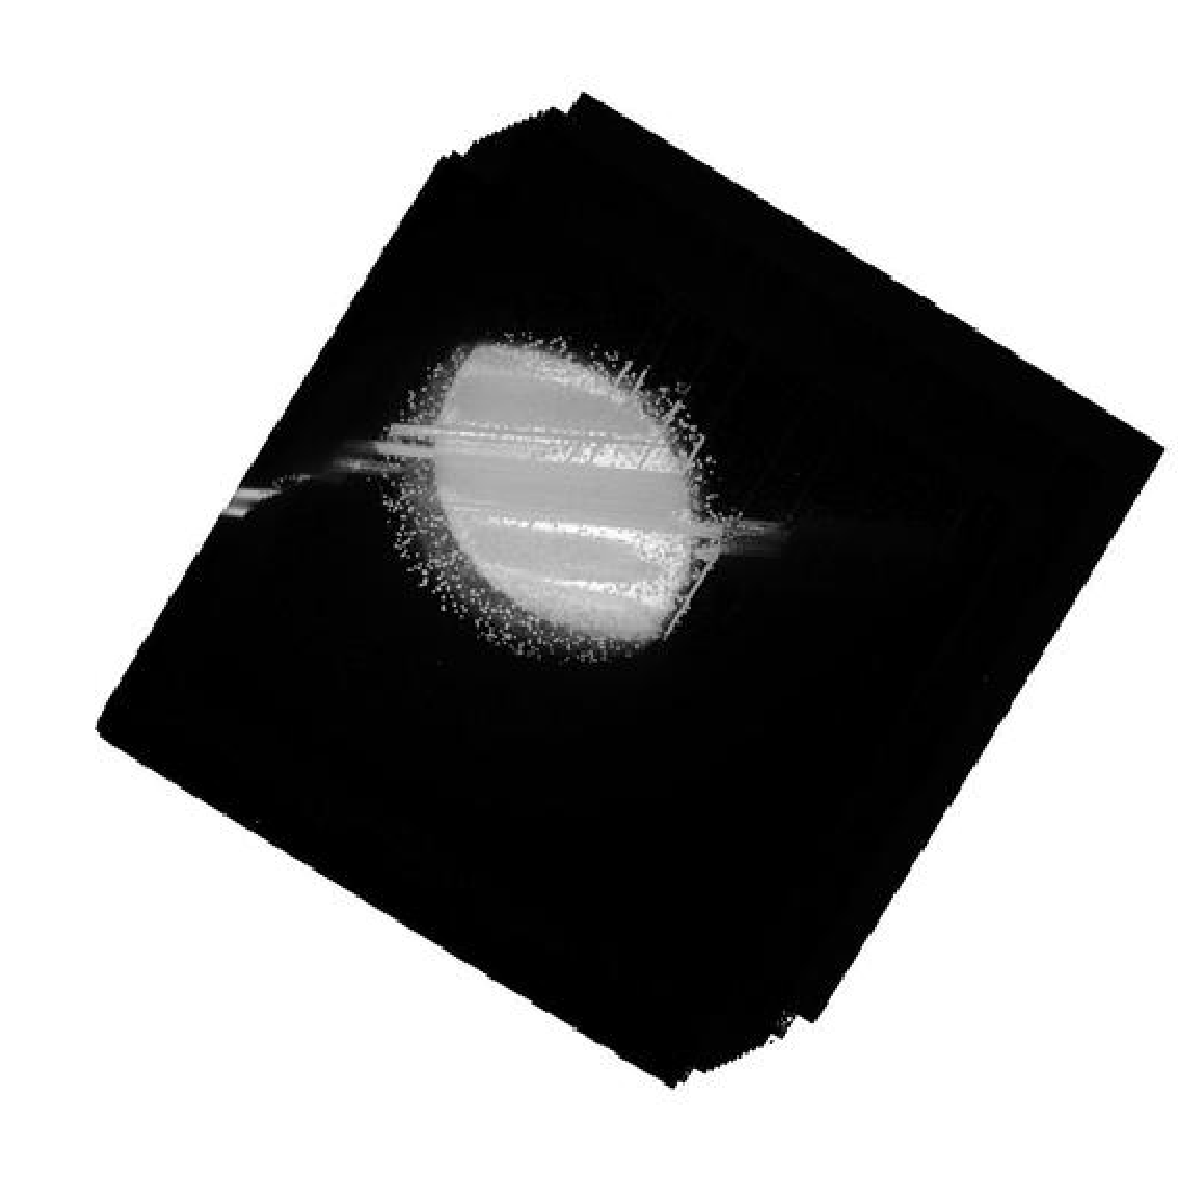
\includegraphics[width=0.18\textwidth]{\thedatafolder/img_tti_0_2.pdf} \\ \input{\thedatafolder/propid_tti_0_2.txt} & \centering 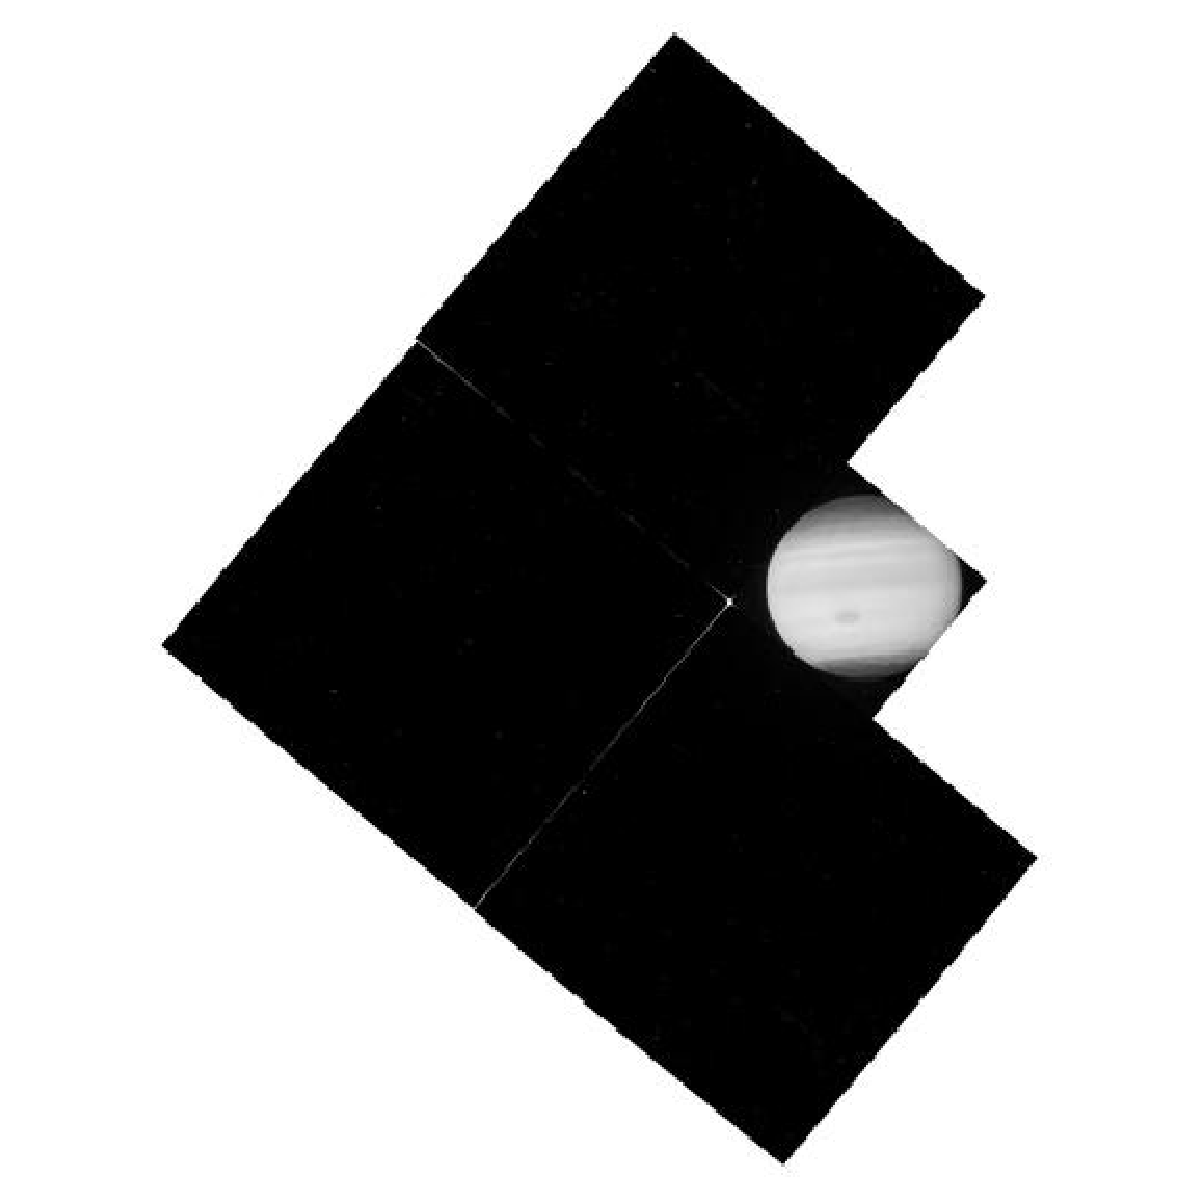
\includegraphics[width=0.18\textwidth]{\thedatafolder/img_tti_0_3.pdf} \\ \input{\thedatafolder/propid_tti_0_3.txt}  \tabularnewline
      \midrule
      \texttt{\input{\thedatafolder/query_tti_2.txt}} \vspace{20mm} & \centering 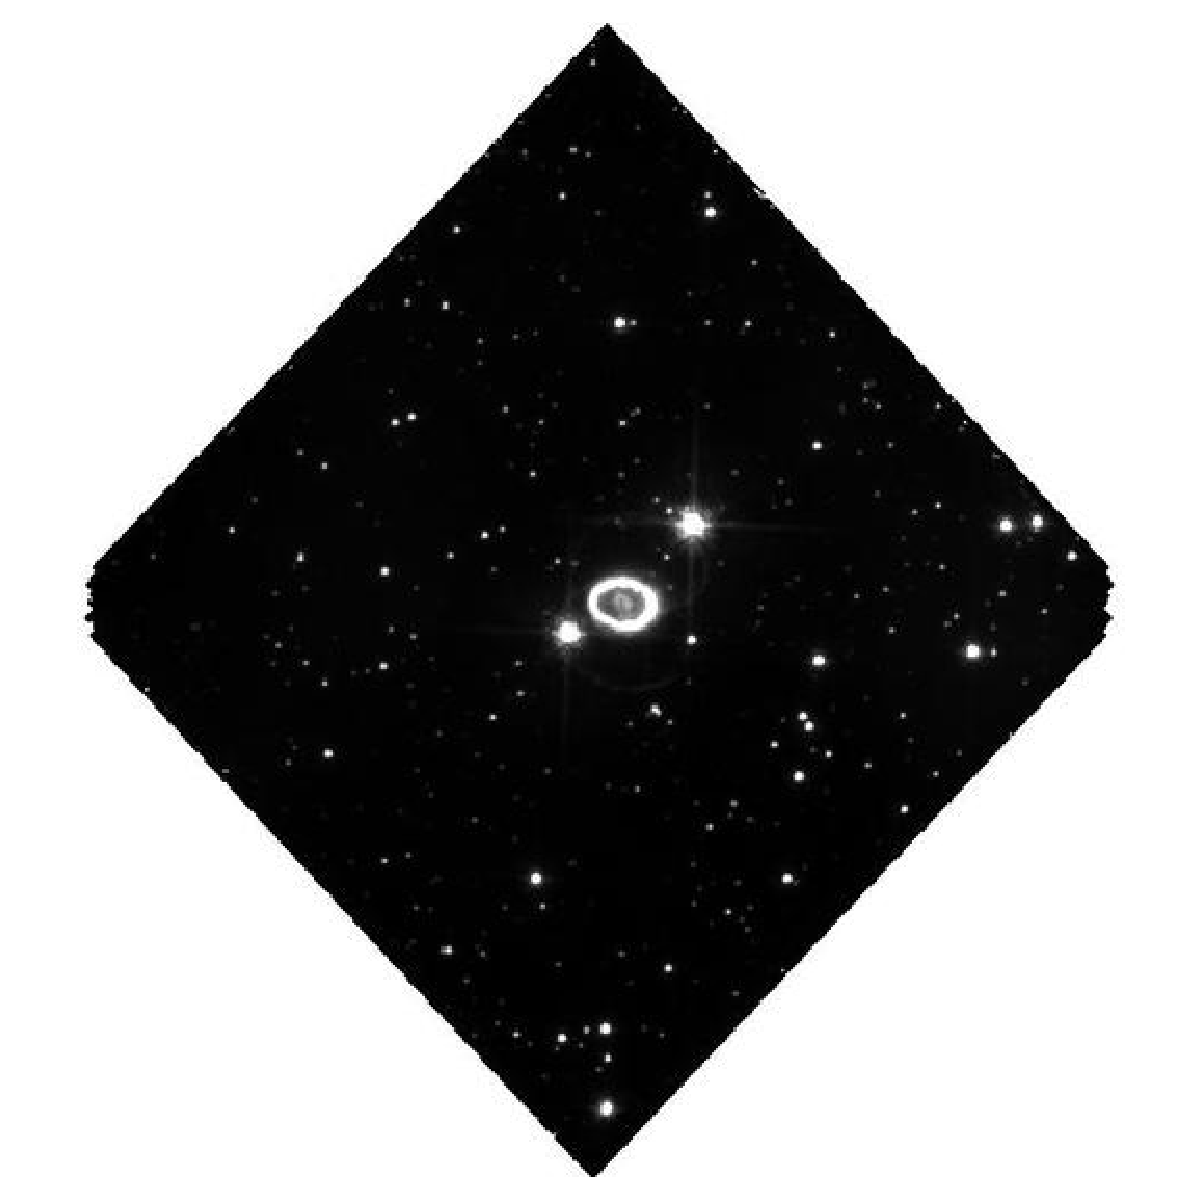
\includegraphics[width=0.18\textwidth]{\thedatafolder/img_tti_2_0.pdf} \\ \input{\thedatafolder/propid_tti_2_0.txt} & \centering 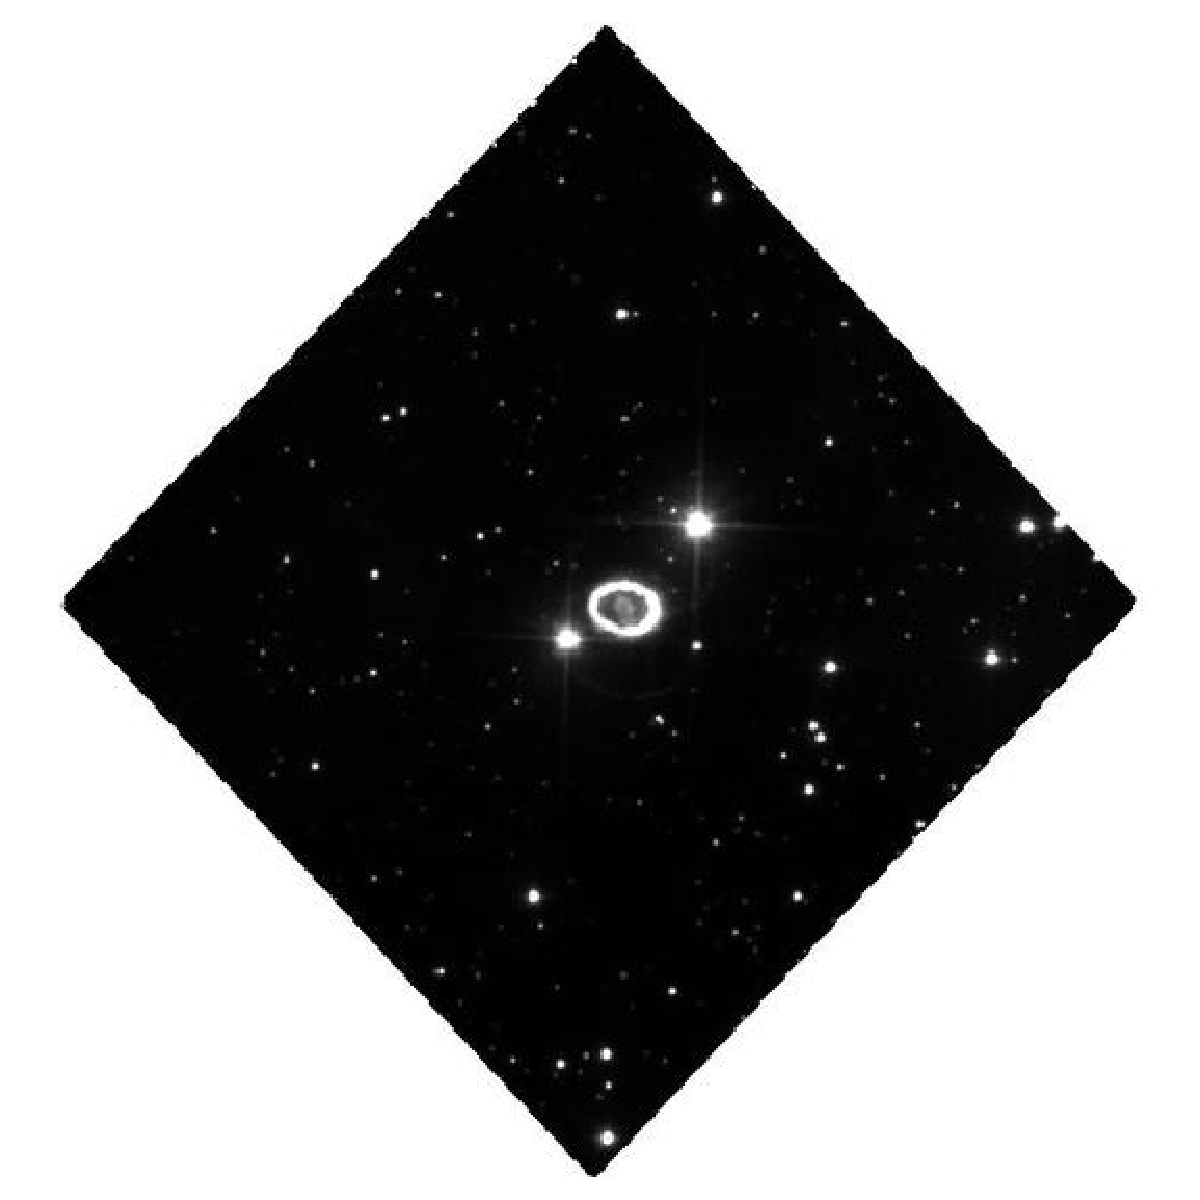
\includegraphics[width=0.18\textwidth]{\thedatafolder/img_tti_2_1.pdf} \\ \input{\thedatafolder/propid_tti_2_1.txt} & \centering 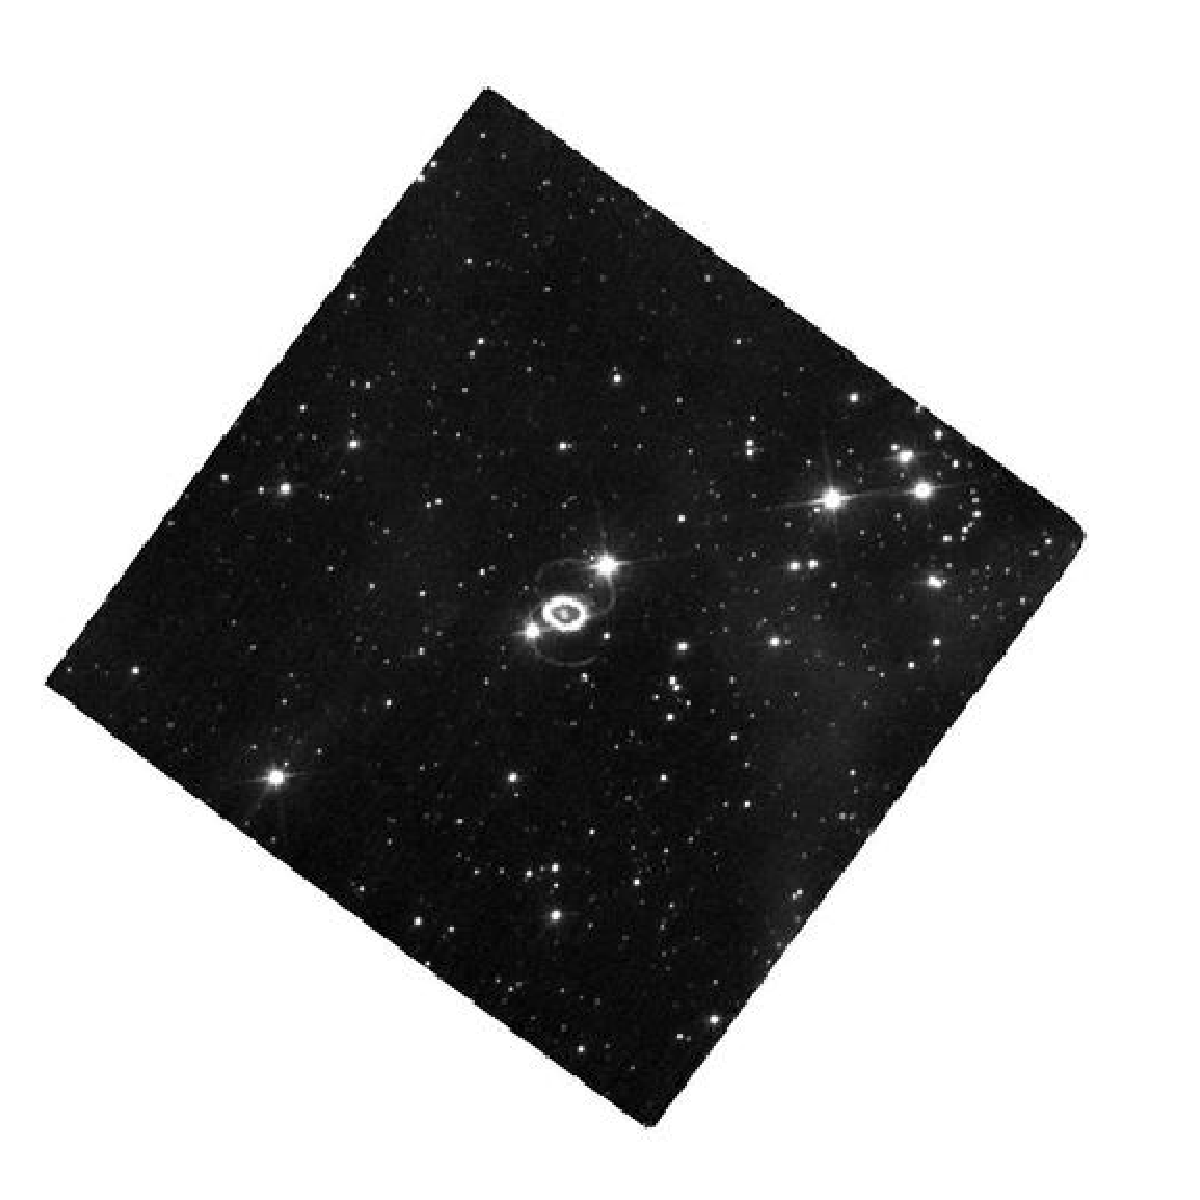
\includegraphics[width=0.18\textwidth]{\thedatafolder/img_tti_2_2.pdf} \\ \input{\thedatafolder/propid_tti_2_2.txt} & \centering 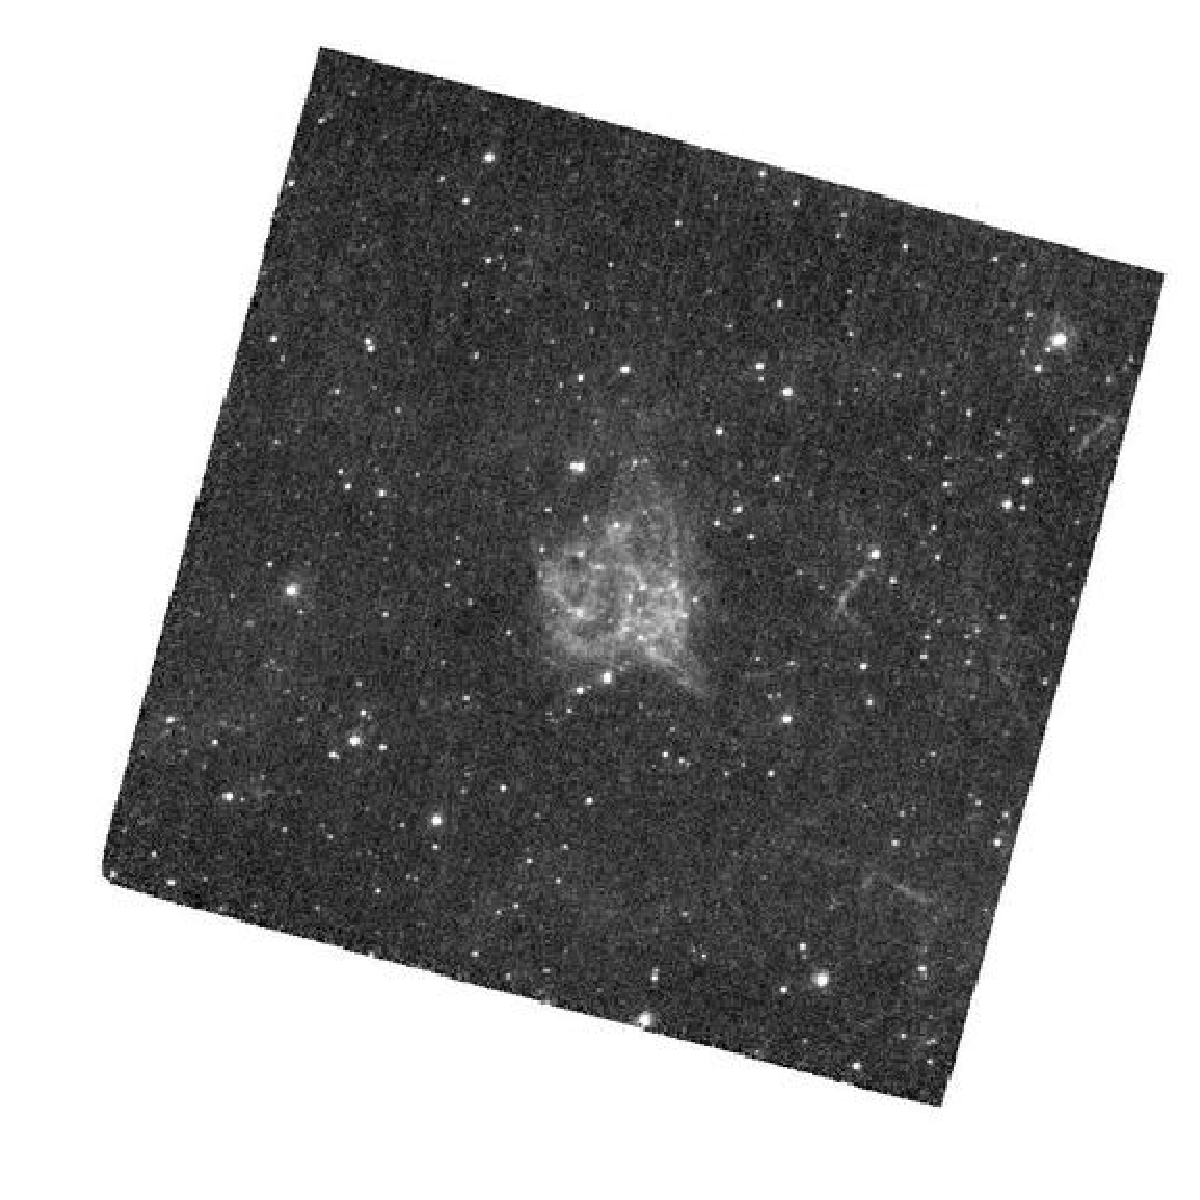
\includegraphics[width=0.18\textwidth]{\thedatafolder/img_tti_2_3.pdf} \\ \input{\thedatafolder/propid_tti_2_3.txt}  \tabularnewline
      \midrule
      \texttt{\input{\thedatafolder/query_tti_3.txt}} \vspace{20mm} & \centering 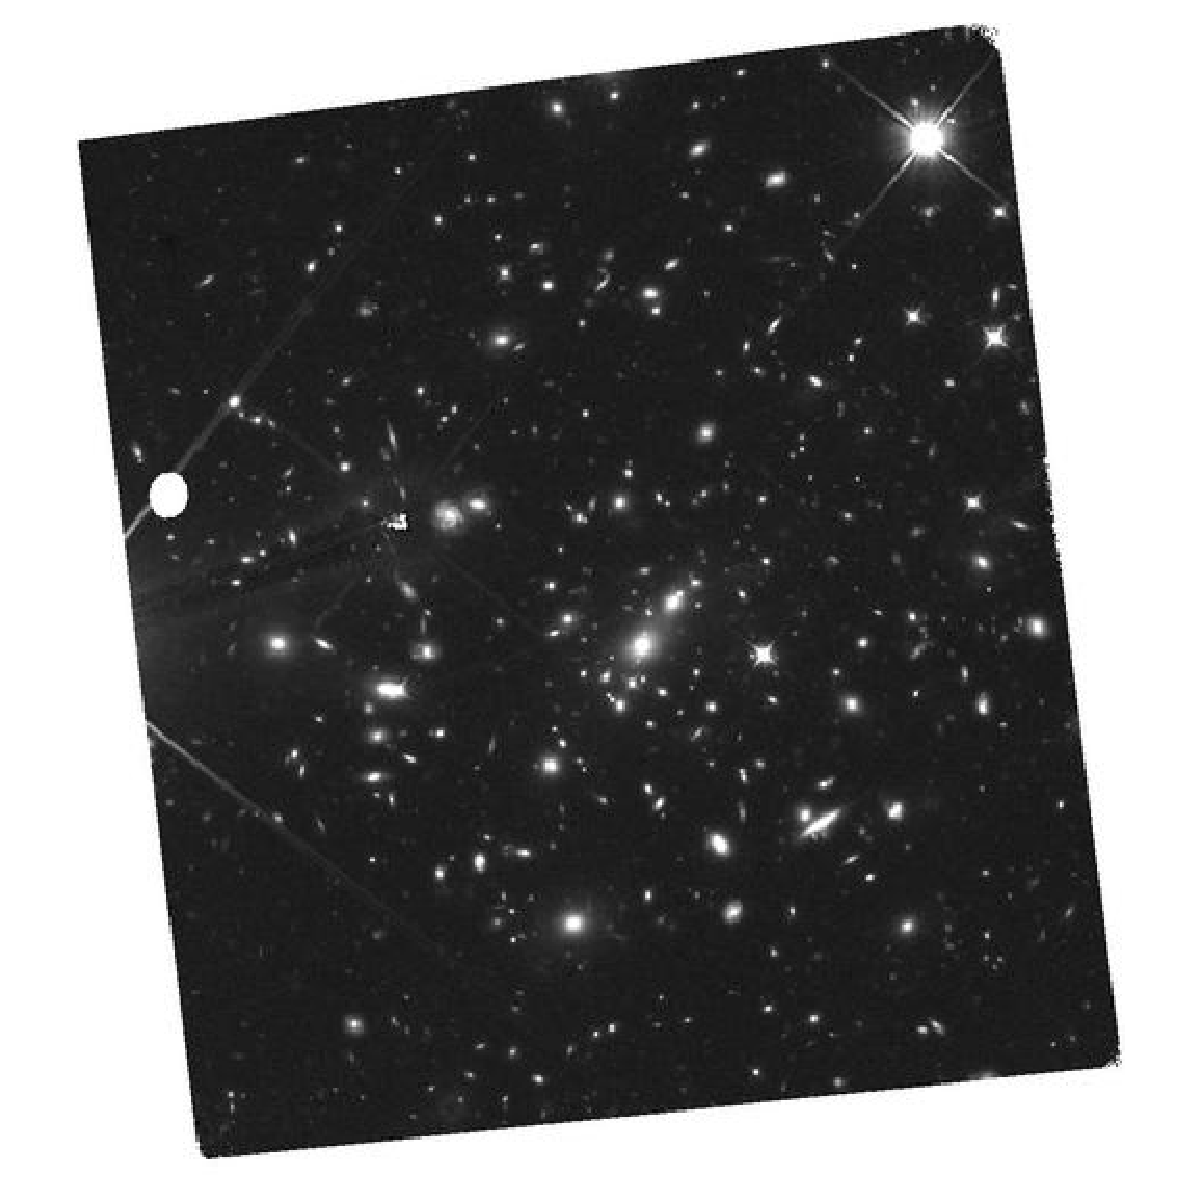
\includegraphics[width=0.18\textwidth]{\thedatafolder/img_tti_3_0.pdf} \\ \input{\thedatafolder/propid_tti_3_0.txt} & \centering 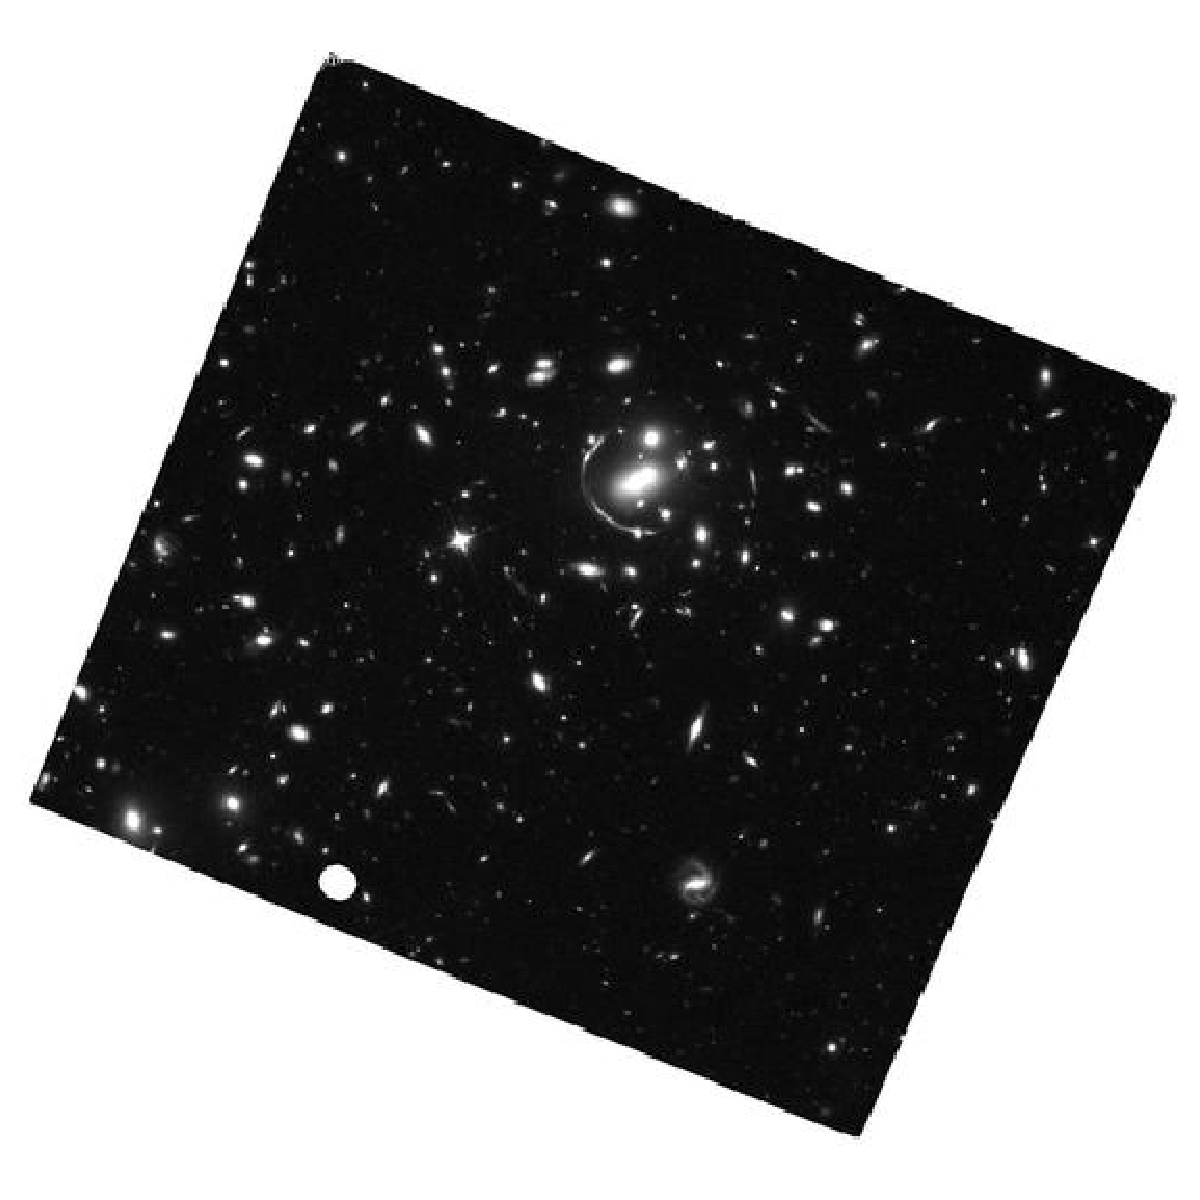
\includegraphics[width=0.18\textwidth]{\thedatafolder/img_tti_3_1.pdf} \\ \input{\thedatafolder/propid_tti_3_1.txt} & \centering 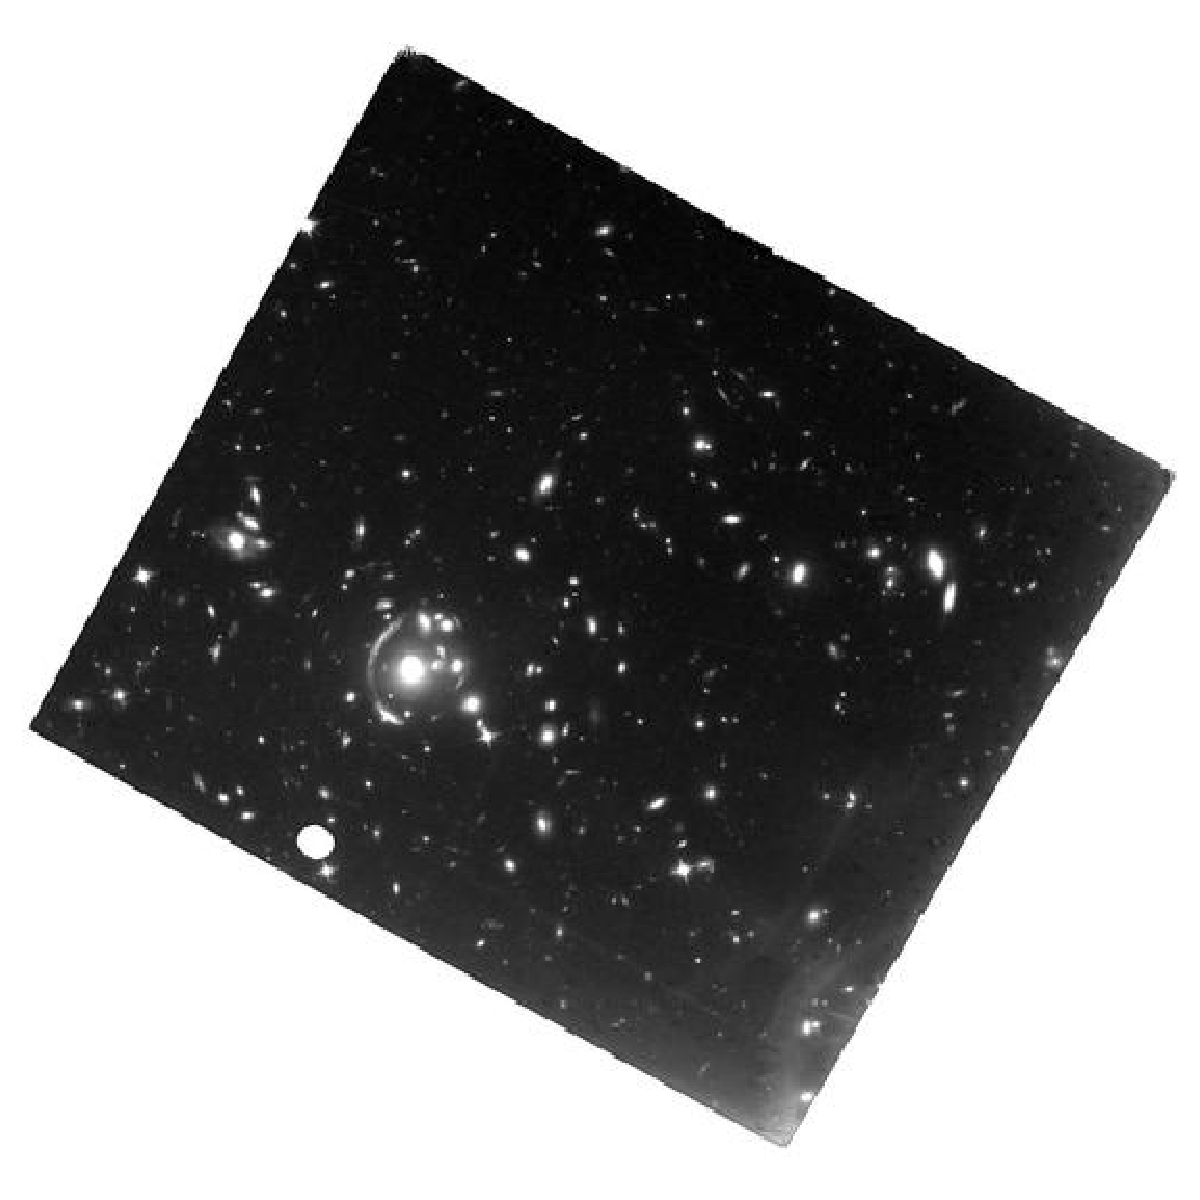
\includegraphics[width=0.18\textwidth]{\thedatafolder/img_tti_3_2.pdf} \\ \input{\thedatafolder/propid_tti_3_2.txt} & \centering 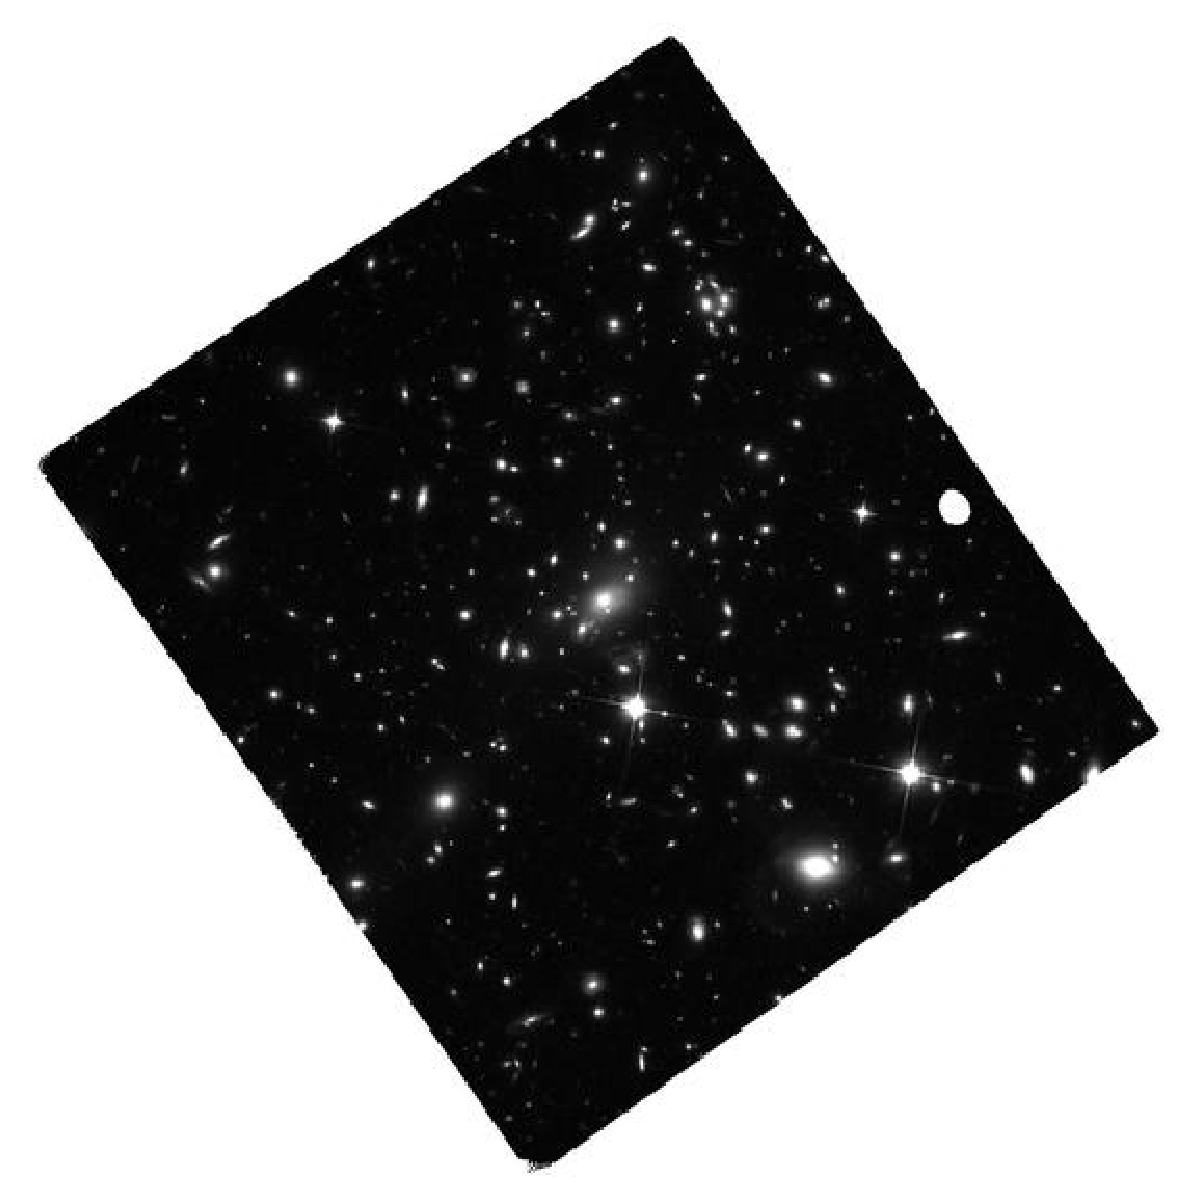
\includegraphics[width=0.18\textwidth]{\thedatafolder/img_tti_3_3.pdf} \\ \input{\thedatafolder/propid_tti_3_3.txt}  \tabularnewline
      \bottomrule
  \end{tabular}
  \caption{Same as Tab.~\ref{tab:tti_base}, but using the \textbf{\textcolor{deepred}{summary fine-tuned CLIP model}}.}
  \label{tab:tti}
\end{table}

% \begin{figure*}[!h]
% 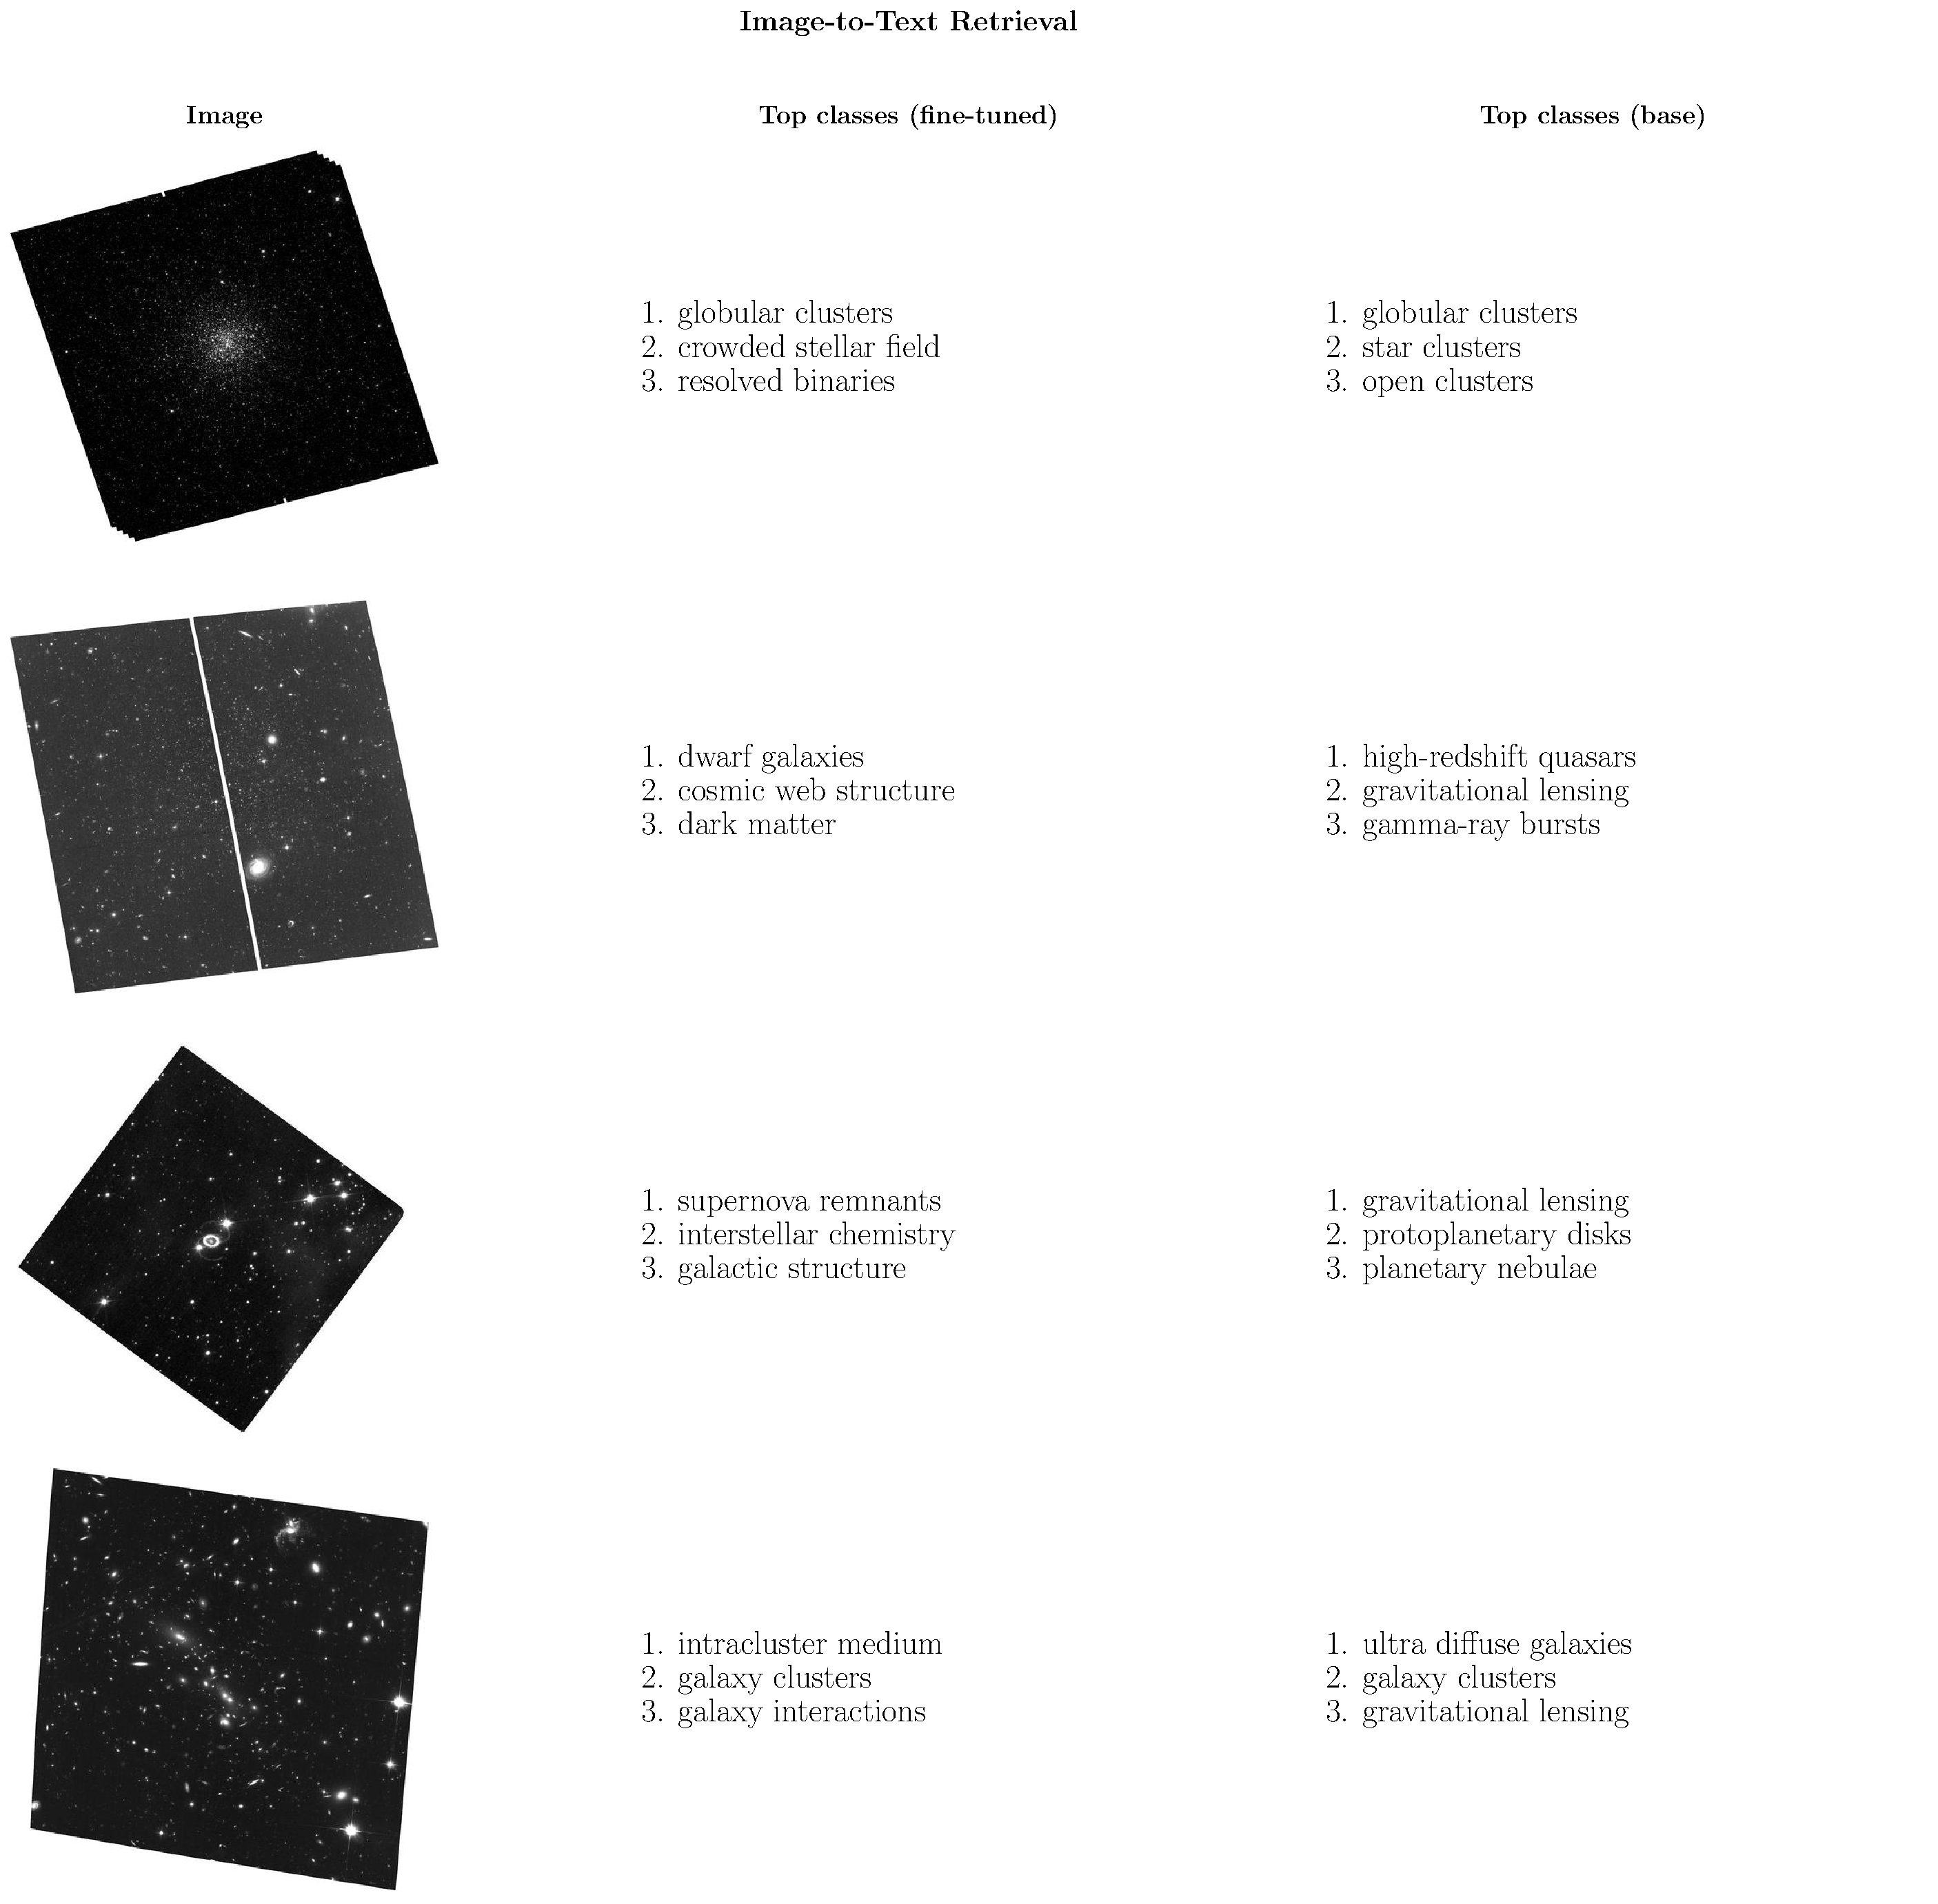
\includegraphics[width=0.95\textwidth]{plots/itt.pdf}
% \caption{Text associations from a curated list most closely matching a given image query, for both the fine-tuned and base models. The `ground truth' LLM-summarized abstract is shown in the right column. \SM{Say ground truth summarized abstract in the column}\SM{Swap order of cols 2 and 3.}}
% \label{fig:itt}
% \end{figure*}

% Set line spacing to 0.5

\begin{table}[h!]
  \centering
  \renewcommand{\arraystretch}{0.1}
  \begin{tabular}{m{3cm} m{3.6cm} m{3.6cm} m{4cm}}
      \toprule
      \centering \bfseries \hubble image & \centering \textbf{Top-4 text} \\ \small\textbf{\textcolor{deeppurple}{(base)}} & \centering  \textbf{Top-4 text} \\ \small\textbf{\textcolor{deepred}{(summary fine-tuned)}} & \centering \textbf{Summarized abstract} \\ (objects; `ground truth') \tabularnewline
      \midrule
      \centering 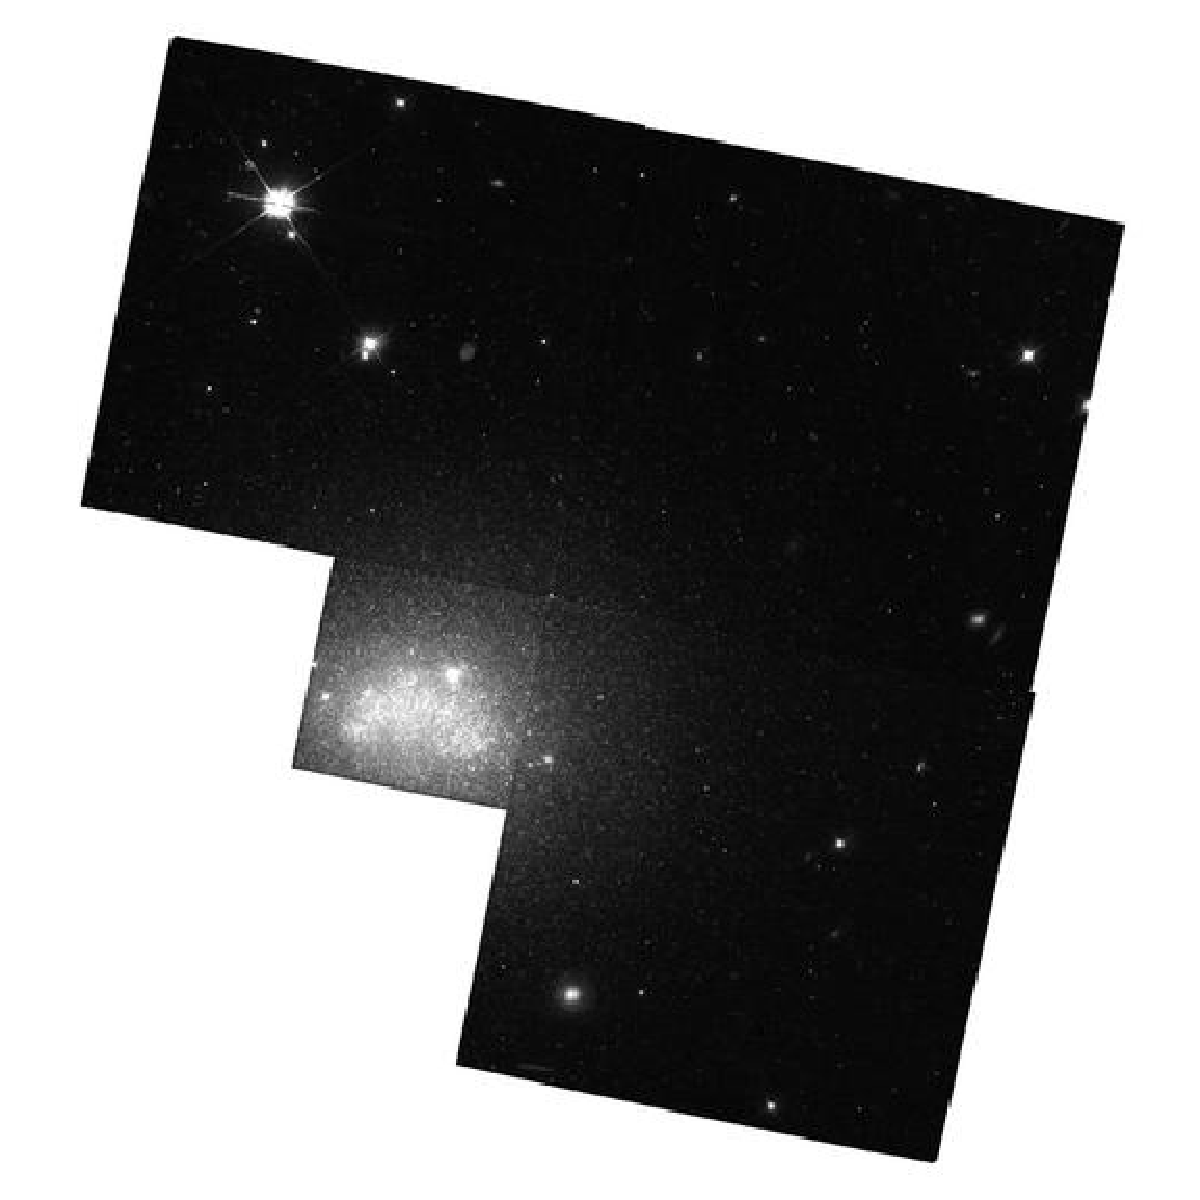
\includegraphics[width=0.15\textwidth]{\thedatafolder/img_itt_0.pdf} & \centering \scriptsize \verbatiminput{\thedatafolder/sci_itt_base_0.txt} & \centering  \scriptsize \verbatiminput{\thedatafolder/sci_itt_0.txt} &  {\scriptsize \input{\thedatafolder/abs_itt_0.txt}} \tabularnewline
      \midrule
      \centering 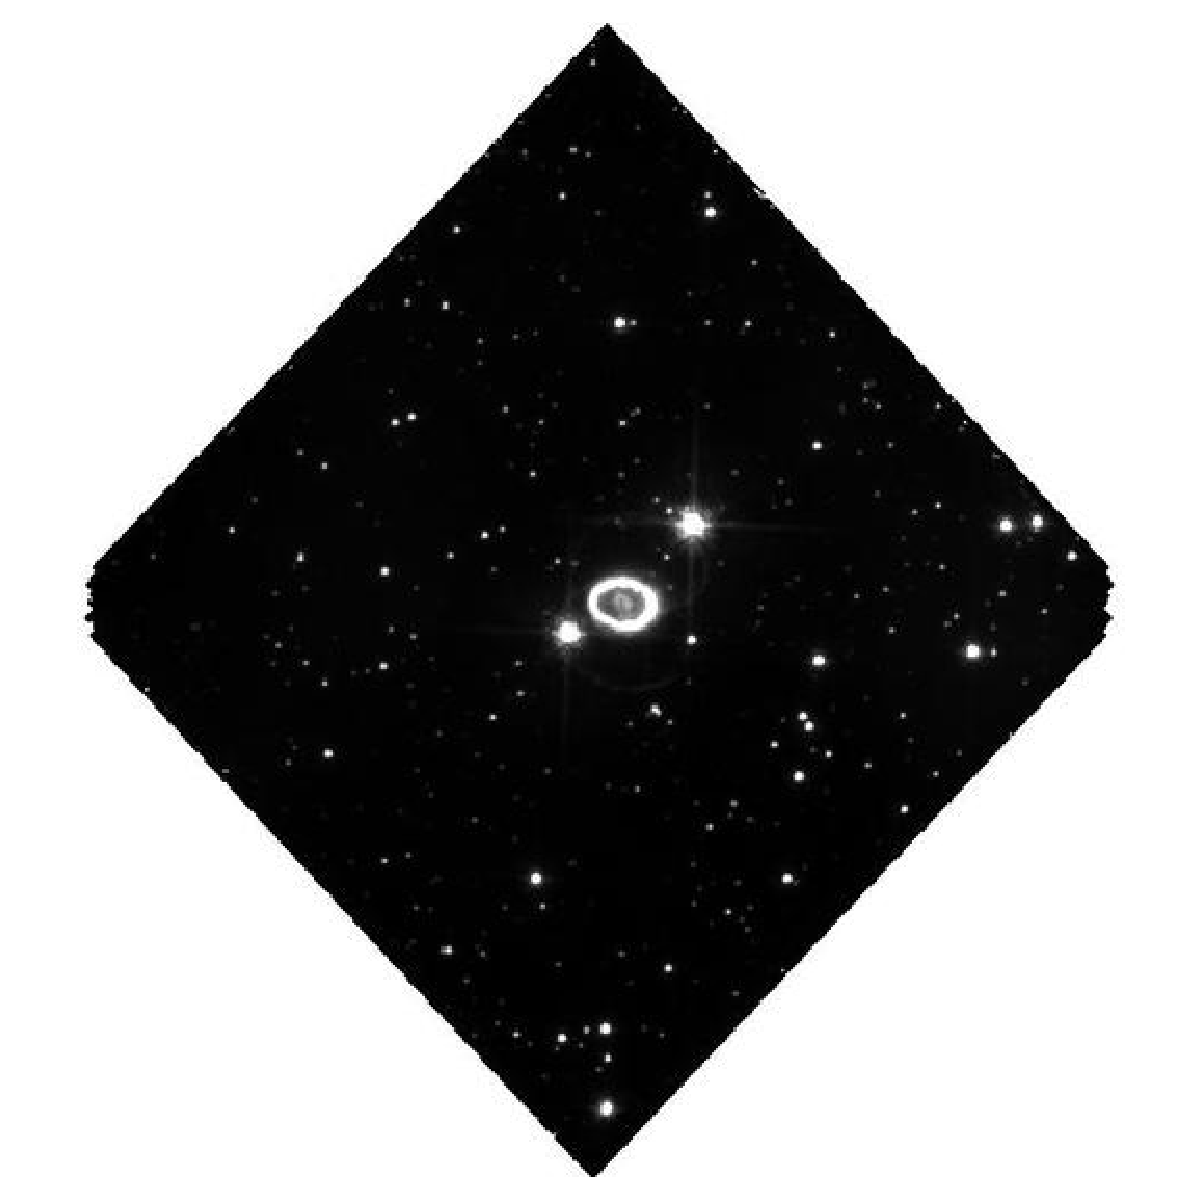
\includegraphics[width=0.15\textwidth]{\thedatafolder/img_itt_1.pdf} & \centering \scriptsize \verbatiminput{\thedatafolder/sci_itt_base_1.txt} & \centering  \scriptsize \verbatiminput{\thedatafolder/sci_itt_1.txt} &  {\scriptsize \input{\thedatafolder/abs_itt_1.txt}} \tabularnewline
      \midrule
      \centering 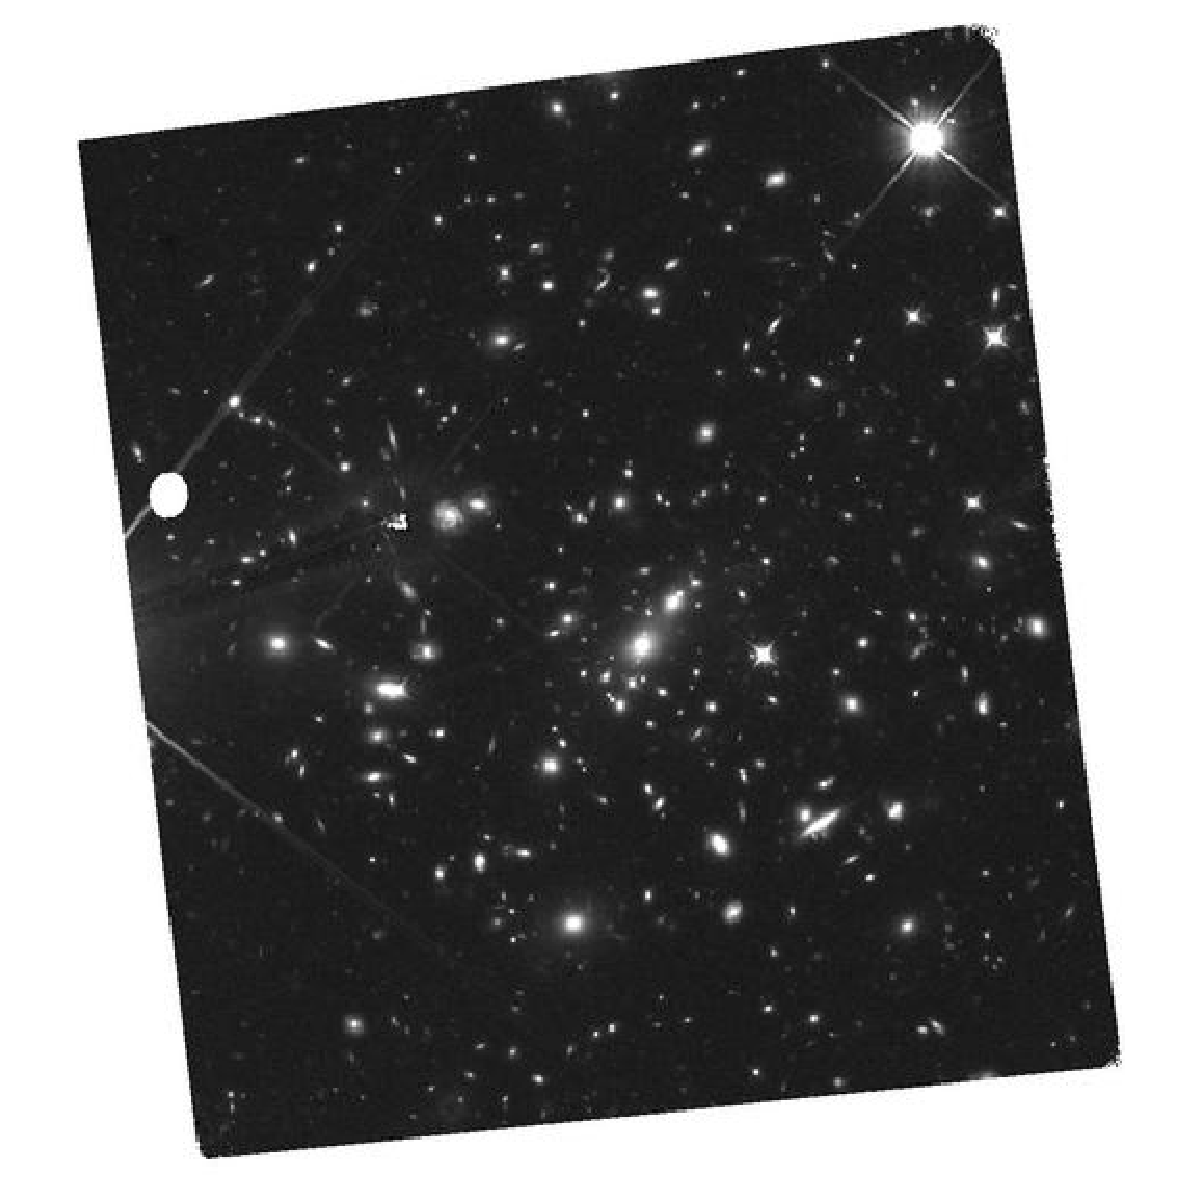
\includegraphics[width=0.15\textwidth]{\thedatafolder/img_itt_2.pdf} & \centering \scriptsize \verbatiminput{\thedatafolder/sci_itt_base_2.txt} & \centering  \scriptsize \verbatiminput{\thedatafolder/sci_itt_2.txt} &  {\scriptsize \input{\thedatafolder/abs_itt_2.txt}} \tabularnewline
      \midrule
      \centering 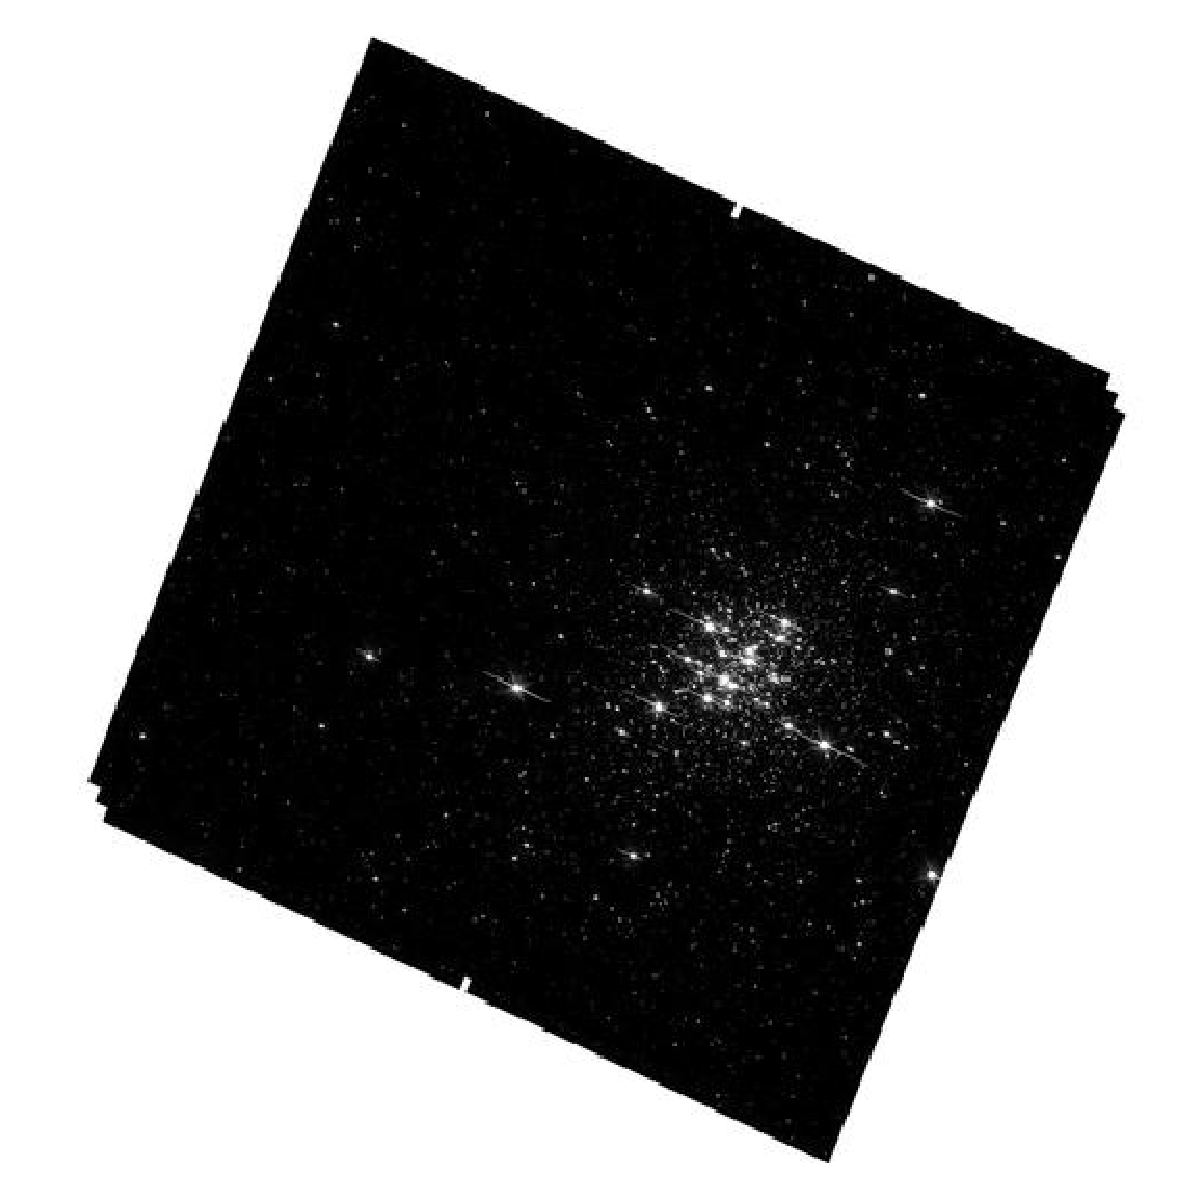
\includegraphics[width=0.15\textwidth]{\thedatafolder/img_itt_3.pdf} & \centering \scriptsize \verbatiminput{\thedatafolder/sci_itt_base_3.txt} & \centering  \scriptsize \verbatiminput{\thedatafolder/sci_itt_3.txt} &  {\scriptsize \input{\thedatafolder/abs_itt_3.txt}} \tabularnewline
      \bottomrule
  \end{tabular}
  \caption{Text snippets from a curated list most closely matching a given image query (left-most column) by cosine similarity, shown for the \textcolor{deeppurple}{base} (CLIP-ViT-B/16) and \textcolor{deepred}{summary fine-tuned} models. The `ground truth' LLM-summarized abstract is shown in the right-most column.}
  \label{tab:itt}
\end{table}

\section{Outlook and Conclusions}
\label{sec:conclusion}

In this paper we present \textsc{PAPERCLIP}, a method for training domain-specific multi-modal models for astrophysics that associates observations imaged by telescopes with natural language in a common, semantically-meaningful embedding space.
%
We showcase an application to \hubble Space Telescope (HST) observations, where the model is fine-tuned from a pre-trained CLIP model using (optionally summarized) abstracts of successful \hubble proposals, leveraging a noisy association signal between text and images.
%
We show that \textsc{PAPERCLIP} significantly outperforms the base CLIP model in quantitative metrics, such as retrieval accuracy, as well as quality of text-to-image and image-to-text retrieval.
%
We also introduce a novel LLM summarization process which leverages guided generation to distill the content of proposal abstracts while preserving salient information. 
%
Overall, the procedure demonstrates the efficacy on fine-tuning generalist pre-trained models on small amounts of domain-specific data, in particular astronomical datasets.

Although the model explored here is fine-tuned using postage stamp images (i.e., preview-quality and not science-grade data), we highlight potential immediate as well as downstream use cases of the PAPERCLIP paradigm.
%
A model trained using weakly-supervised image-text pairs can be used to query survey data e.g., PHANGS~\citep{lee2022phangs}, COSMOS~\citep{scoville2007cosmic} using natural language, as well as to quickly find distinguishing patterns in such data that may not be apparent using specialized models or manual inspection.
%
The learned representations, having shown to correlate with physical characteristics of imaged objects, can also be fine-tuned via transfer learning to adapt to either specific tasks e.g., classification~\citep{wei2020deep} or segmentation~\citep{hausen2020morpheus}, or observations imaged by other telescopes.
%

Finally, while the CLIP model is restricted to retrieving nearest-neighbour associations within and across text/image modalities, the learned embeddings can be used as a starting point for training or fine-tuning multi-modal large-language models for interacting with survey data and receiving responses in natural language form, as well as grounding the responses based on an existing set of observations.

\subsubsection*{Code and Data Availability}

The code, dataset, and fine-tuned models used in this work are available at \url{https://www.github.com/smsharma/HubbleCLIP}.

\subsubsection*{Sofware}

This work relied on the \package{Astroquery} \citep{2019AJ....157...98G}, \package{BitsAndBytes} \citep{dettmers2022llmint8}, \package{Flax} \citep{flax2020github}, \package{Jax} \citep{jax2018github}, \package{Jupyter} \citep{Kluyver2016jupyter}, \package{Matplotlib} \citep{Hunter:2007}, \package{Numpy} \citep{harris2020array}, \package{Optax} \citep{deepmind2020jax}, \package{Outlines}, \package{Pandas} \citep{2020SciPy-NMeth}, \package{Pydantic}, \package{PyTorch} \citep{paszke2019pytorch}, \package{SciPy} \citep{2020SciPy-NMeth}, \package{Transformers} \citep{wolf2019huggingface}, and \package{Wandb} \citep{wandb} software packages.

% Code repo and package cites.
% Dataset availability

\subsubsection*{Broader Impact}

This work relies on using abstracts from successful \hubble Space Telescope observing proposals to fine-tune machine learning models. While these abstracts are publicly accessible, the authors likely did not anticipate their text being used to train machine learning models, raising questions around consent and appropriate use of data. Since this research intends to develop methods to aid astronomical research and does not use sensitive personal information or target commercial gain, we believe that the scientific benefits outweigh the potential concerns in this case while acknowledging good-faith arguments to the contrary. As the use of foundation models in the sciences increases, it will be important for the astronomy community to consider norms and guidelines around the appropriate use of various data sources for model training to ensure transparency and maintain trust in the community.

\subsubsection*{Acknowledgments}

We thank Michael Brenner for helpful conversations.
%
This work is supported by the National Science Foundation under Cooperative Agreement PHY-2019786 (The NSF AI Institute for Artificial Intelligence and Fundamental Interactions, \url{http://iaifi.org/}).
%
This material is based upon work supported by the U.S. Department of Energy, Office of Science, Office of High Energy Physics of U.S. Department of Energy under grant Contract Number  DE-SC0012567. 
%
YS was supported by the Research Science Institute (RSI) program at MIT.
%
This research was supported by an award from Google,  ``Interpretation of Multimodal Images from Astronomy''.
%
This research was supported by the Munich Institute for Astro-, Particle and BioPhysics (MIAPbP), which is funded by the Deutsche Forschungsgemeinschaft (DFG, German Research Foundation) under Germany's Excellence Strategy – EXC-2094 – 390783311.
%
The computations in this paper were run on the FASRC Cannon cluster supported by the FAS Division of Science Research Computing Group at Harvard University.

This research is based on observations made with the NASA/ESA Hubble Space Telescope obtained from the Space Telescope Science Institute, which is operated by the Association of Universities for Research in Astronomy, Inc., under NASA contract NAS 5-26555.

Based on observations made with the NASA/ESA Hubble Space Telescope, and obtained from the Hubble Legacy Archive, which is a collaboration between the Space Telescope Science Institute (STScI/NASA), the Space Telescope European Coordinating Facility (ST-ECF/ESAC/ESA) and the Canadian Astronomy Data Centre (CADC/NRC/CSA).


\bibliography{main}
\bibliographystyle{tmlr}

\appendix

\section{Details on the Abstract Summarization Procedure}

\subsection{Guided LLM Generation with \package{Outlines}}
\label{app:guided-generation}

We employ the guided generation method introduced by \citet{willard2023efficient} and implemented in \package{Outlines} to ensure that the LLM summarization of the raw proposal abstracts adheres to specific pattern, specified in JSON format (Sec.~\ref{app:summarization} below), which we briefly describe here. This approach represents the desired output format as a finite-state machine (FSM) that encodes the JSON schema as a regular expression. The JSON schema constraint is therefore first converted into a regular expression.

The key idea then is to pre-compute an index that maps each state of the FSM to the subset of tokens from the LLM's vocabulary that can be generated from that state while still allowing for a valid completion of the pattern. By doing so, we can efficiently determine the valid next tokens at each step of the generation process without having to check the entire vocabulary.

Formally, let $\mathcal{M} = (Q, \Sigma, \delta, q_0, F)$ be the FSM representing the regular expression, where $Q$ is the set of states, $\Sigma$ is the alphabet of the regular expression, $\delta: Q \times \Sigma \rightarrow Q$ is the transition function between states, $q_0$ is the start state, and $F$ is the set of accept states which terminate the generation. An index $\sigma: Q \rightarrow \mathcal{P}(V)$ is first constructed, where $V$ is the LLM's token vocabulary and $\mathcal{P}(V)$ denotes the power set of $V$. For each state $q \in Q$, $\sigma(q)$ contains the allowed tokens that can be generated from state $q$ while maintaining the possibility of reaching an accept state. The construction of $\sigma$ involves finding all token sequences that, when processed by the FSM starting from each state $q$, lead to an accept state.

During the token-by-token generation process, we keep track of the current FSM state $q_t$ after sampling each token $v_t$. At each step $t$, we mask the LLM's output logits based on the valid next tokens $\sigma(q_t)$, setting the logits of invalid tokens to $-\infty$. The next token is then sampled from the categorical distribution defined by the unmasked logits, and the FSM transitions to the next state $q_{t+1} = \delta(q_t, v_{t+1})$, where $v_{t+1} \in \Sigma$ is the token in the regular expression alphabet corresponding to the sampled token. This process continues until an accept state with no outgoing transitions is reached, indicating a valid completion of the pattern.

% The regex-guided generation method ensures that the LLM's output always adheres to the specified regular expression pattern, without incurring the computational overhead of checking the validity of each possible next token at every generation step. This approach can be extended to more complex patterns, such as context-free grammars, by using augmented pushdown automata to track the generation state and valid next tokens.

% In our application, we use the regex-guided generation method to constrain LLM outputs to follow specific JSON schemas, which are automatically converted into regular expressions. This ensures that the generated summaries of astronomy observation proposals adhere to the desired format, enabling more reliable extraction of key information.
% The pre-computed index $\sigma$ allows for efficient determination of valid next tokens at each generation step, making the regex-guided method computationally feasible for large-scale applications. 

\subsection{Prompts and Schema Used for Summarization}
\label{app:summarization}

We list here the prompts and schema (i.e.
%
desired output formats) used for guided text generation via \package{Outlines} package interfacing with the \textsc{Mixtral-8x7B-Instruct} open-weights LLM.

The following schema is used to guide the generation of the summaries, intended to produce between one and five objects and hypotheses, as well as science use cases.

\begin{lstlisting}[language=Python]
from pydantic import BaseModel, conlist

class ConstrainedResponseHST(BaseModel):
      objects_and_phenomena: conlist(str, min_length=1, max_length=5)
      science_use_cases: conlist(str, min_length=1, max_length=5)
\end{lstlisting}

The following prompt is used to produce a list of possible objects and phenomena shown in HST observations downstream of a proposal abstract, as well as one to five possible science use cases.

\begin{lstlisting}[language=Python]
import outlines 

@outlines.prompt
def prompt_fn(abstract):
      """<s>[INST] You are an expert astrophysicist, with broad expertise across observational and theoretical astrophysics. You are able to extract core information from astrophysical texts.

Abstract: "{{abstract}}"

Based on the above observational proposal abstract, your task is to summarize the nature of the eventual observations. You will identify the astrophysical objects and phenomena, as well as the potential science use cases described in the abstract.

Follow these instructions exactly:
- Mention up to 5 items for both categories; do not mention more than 5 items in either category. 
- Choose the most relevant ones if there are more than 5 items in a category.
- Never mention the Hubble Space Telescope, HST, or the HST archive.
- Mention the class (e.g., barred spiral galaxy) and not just the specific instance (e.g., Andromeda).
- Name the objects in the science use cases, if appropriate.
- Write out full names of objects in addition to acronyms.
- Do not list irrelevant objects which do not describe the eventual observation, such as units or proposal Cycle numbers. List fewer but more relevant objects, if in doubt.
- Each science case listed must be self-contained but succinct.
- Only write in English.
- Do not list items that are too generic (e.g., galaxy, faint object, kinematics)
- The total length of text should not exceed 80 words.
- Present your lists in a comma-separated format; no dashed or numbered lists.

Example output: {'objects_and_phenomena':'spiral galaxies, galaxy clusters, supernova remnants', 'science_use_cases':'model galactic structure and evolution, characterize dark matter distribution in clusters, analyze expansion rates of supernova remnants'}

Answer in JSON format. The JSON should be a dictionary with keys "objects_and_phenomena" and "science_use_cases".

[/INST]
"""
\end{lstlisting}

% \subsection{Generation of single-concept summaries}
% \label{app:singleconcept}

% The following prompt is used to generate a list of diverse single-concept summaries informed by a list of summarized abstracts:

% \begin{lstlisting}[language=Python]
% import outlines   

% @outlines.prompt
% def prompt_fn(objects):
%     """<s>[INST] Please produce a list of around concepts characterizing prominent objects, phenomena, and science use cases of images observed by the Hubble Space Telescope.

% Here are some examples of objects:

% {{objects}}

% Follow these instructions exactly in your answer:
% - Do not output empty strings as elements.
% - Make sure that the list covers a diverse range of astronomical concepts, with items as different from each other as possible. 
% - Do not give specific names of objects, to make sure you span the widest possible range of concepts (e.g., "dwarf galaxy" is allowed, but NOT "Fornax", "Terzan 5", or  "NGC6440").
% - Do not return terms undescriptive of observations, e.g. "sloshing", "adiabatic", "interactions". Returning concrete physics objects, concepts, or phenomena.
% - Only output scientifically meaningful terms. E.g., NO "Cosmic Dance".
% - Do not duplicate entries. Do not reference any telescopes, observatories, or surveys.
% - Do not include units like "angular diameter distance", "parsec", or any other concepts that will not correlate with images of observations.
% - Use the above example list of objects only as inspiration to infer broad classes of objects.
% - Make sure each concept is succint, never more than 5 words.
% - Answer in JSON format.
% - The JSON should have the following keys {"galaxies", "stellar_physics", "exoplanets_planet_formation", "stellar_populations", "supermassive_black_holes", "solar_system", "integalactic_medium", "large_scale_structure"} reflecting rough observation categories.
% - Each category will have a list of objects and/or astronomical concepts.
% - Output up to 20 items and no more in each category
% [/INST]
% """
% \end{lstlisting}

% The following schema guides generation, intended to produce 100 concepts reflecting the science categories of successful proposals\footnote{\url{https://www.stsci.edu/contents/newsletters/2023-volume-40-issue-02/hubble-cycle-31-proposal-selection}}.
% %


% \begin{lstlisting}[language=Python]
% from pydantic import BaseModel, conlist
  
% class ScienceCategoriesHST(BaseModel):
%     galaxies: conlist(str, min_length=15, max_length=15)
%     stellar_physics: conlist(str, min_length=15, max_length=15)
%     exoplanets_planet_formation: conlist(str, min_length=15, max_length=15)
%     stellar_populations: conlist(str, min_length=10, max_length=10)
%     supermassive_black_holes: conlist(str, min_length=15, max_length=15)
%     solar_system: conlist(str, min_length=10, max_length=10)
%     integalactic_medium: conlist(str, min_length=10, max_length=10)
%     large_scale_structure: conlist(str, min_length=10, max_length=10)
%   \end{lstlisting}

% The output is then constrained to be one of the fixed number of concepts.
  
% \subsection{Assignment of abstracts to single-concept categories}
% \label{app:singleconceptassignments}

% Finally, the following prompt is used to assign concepts inferred in \ref{app:singleconcept} to each abstract:

% \begin{lstlisting}[language=Python]
% import outlines 

% @outlines.prompt
% def prompt_fn(abs, cats):
%     """<s>[INST] The following is a successful proposal abstract for the Hubble Space Telescope: "{{abs}}"

% The following is a list of categories (astronomical concepts) that this abstract could correspond to.

% {{cats}}

% Please answer which of these listed concepts best describes this proposal, based on the objects and phenomena mentioned in the abstract.
% The concept should meaningfully be present in the abstract and the eventual observation.

% - For example, "The locations of supernovae {SNe} in the local stellar and gaseous environment in galaxies, as measured in high spatial resolution WFPC2 and ACS images, contain important clues to their progenitor stars." should return "supernova".
% - If the abstract centers calibration and/or instrumentation efforts, return calibration or instrumention".

% If no concept make sense, return "None". [/INST]
% """
% \end{lstlisting}

\section{List of Categories for Text Retrieval Task}
\label{app:categories}

The following curated categories are used in the text retrieval experiment in Sec.~\ref{sec:results}.
%
These are derived by prompting \textsc{Claude 2}, without any external input (e.g. proposal abstracts) to produce a list of categories corresponding to typical HST observations.

\begin{lstlisting}[language=Python]
  ["star forming galaxies", "lyman alpha", "dust", "crowded stellar field", "core-collapse supernova", "cosmology", "gravitational lensing", "supernovae", "diffuse galaxies", "globular clusters", "stellar populations", "interstellar medium", "black holes", "dark matter", "galaxy clusters", "galaxy evolution", "galaxy formation", "quasars", "circumstellar disks", "exoplanets", "Kuiper Belt objects", "solar system objects", "cosmic web structure", "distant galaxies", "galaxy mergers", "galaxy interactions", "star formation", "stellar winds", "brown dwarfs", "white dwarfs", "nebulae", "star clusters", "galaxy archeology", "galactic structure", "active galactic nuclei", "gamma-ray bursts", "stellar nurseries", "intergalactic medium", "dark energy", "dwarf galaxies", "barred spiral galaxies", "irregular galaxies", "starburst galaxies", "low surface brightness galaxies", "ultra diffuse galaxies", "circumgalactic medium", "intracluster medium", "cosmic dust", "interstellar chemistry", "star formation histories", "initial mass function", "stellar proper motions", "binary star systems", "open clusters", "pre-main sequence stars", "protostars", "protoplanetary disks", "jets and outflows", "interstellar shocks", "planetary nebulae", "supernova remnants", "red giants", "Cepheid variables", "RR Lyrae variables", "stellar abundances", "stellar dynamics", "compact stellar remnants", "Einstein rings", "trans-Neptunian objects", "cosmic microwave background", "reionization epoch", "first stars", "first galaxies", "high-redshift quasars", "primordial black holes", "resolved binaries", "binary stars"]
\end{lstlisting}

% \section{Additional Evaluation Metrics and Ablations}
% \label{app:ablations}

\section{Evaluation of Model Trained on Raw Abstracts}
\label{app:eval_raw}

In the main text, we illustrated qualitative evaluation (image and text retrieval) for the model fine-tuned on summarized abstracts. Here, we show the same for the model fine-tuned on raw proposal abstracts. Table~\ref{tab:tti_abs} shows the top-4 most similar images for the abstract fine-tuned CLIP model on the same curated queries as in Tab.~\ref{tab:tti} for the summary fine-tuned model. Table~\ref{tab:itt_abs} shows text associations from the curated list most closely matching the image queries, for the base and abstract fine-tuned models, as well as the summary fine-tuned model, for comparison. Although qualitatively different behavior is observed for both tasks, the objects retrieved are seen to correspond well the given image/text queries.

\begin{table}[h!]
  \centering
  \begin{tabular}{m{3cm} p{3cm} p{3cm} p{3cm} p{3cm}}
      \toprule
      \centering \bfseries Query & \multicolumn{4}{c}{\bfseries{Top-4 most similar images using \textcolor{deepblue}{abstract fine-tuned CLIP model}}} \tabularnewline
      \midrule
      \texttt{\input{\thedatafolder/query_tti_abs_1.txt}} \vspace{20mm} & \centering 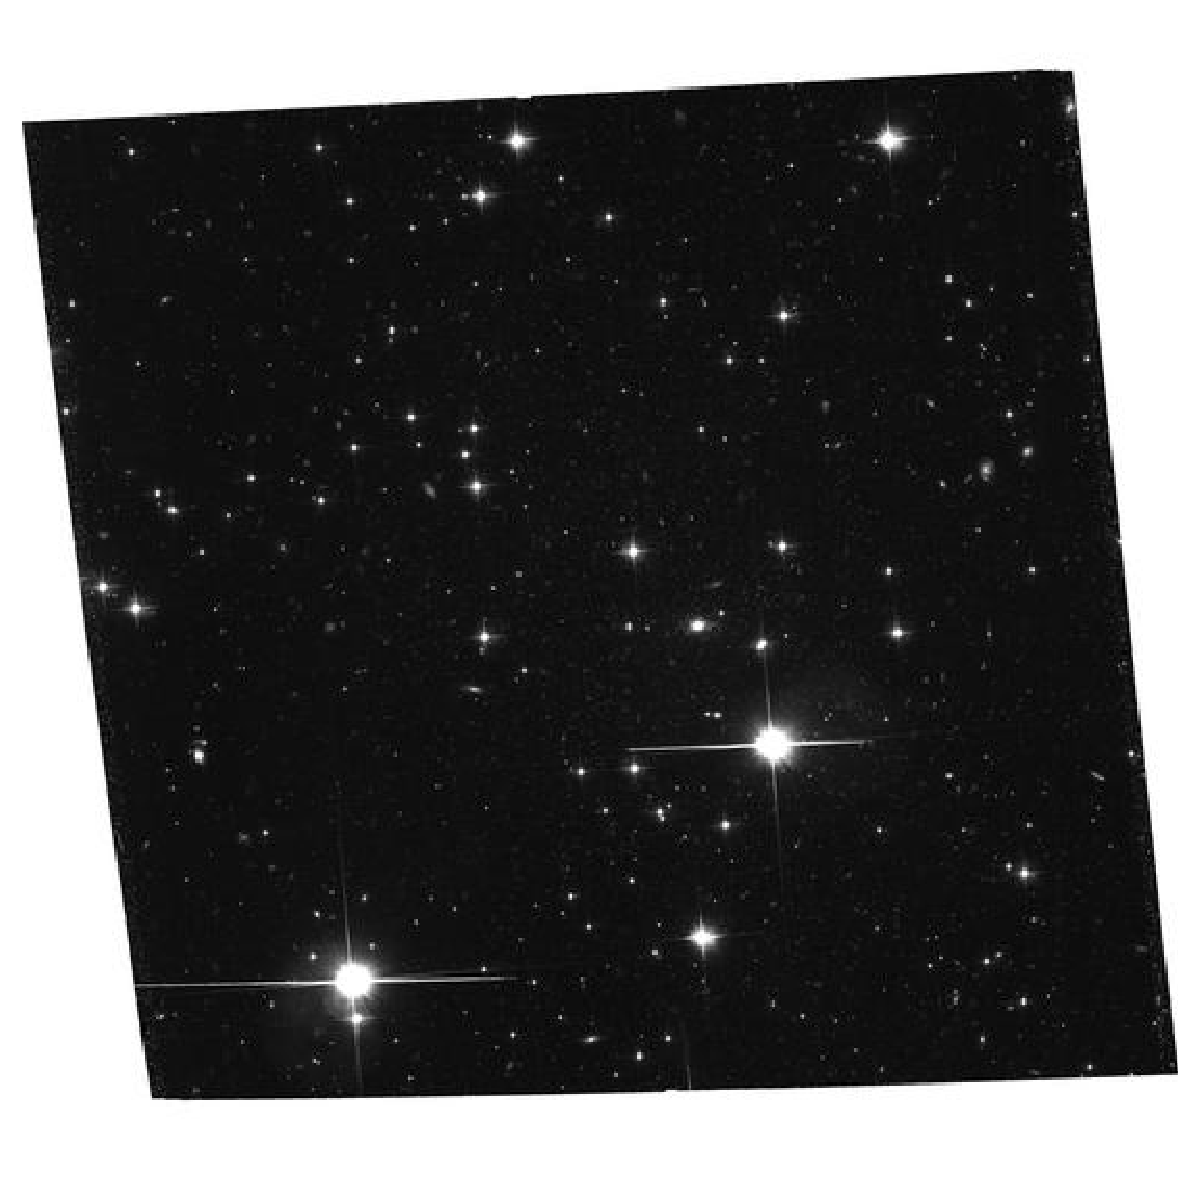
\includegraphics[width=0.18\textwidth]{\thedatafolder/img_tti_abs_1_0.pdf} \\ \input{\thedatafolder/propid_tti_abs_1_0.txt} & \centering 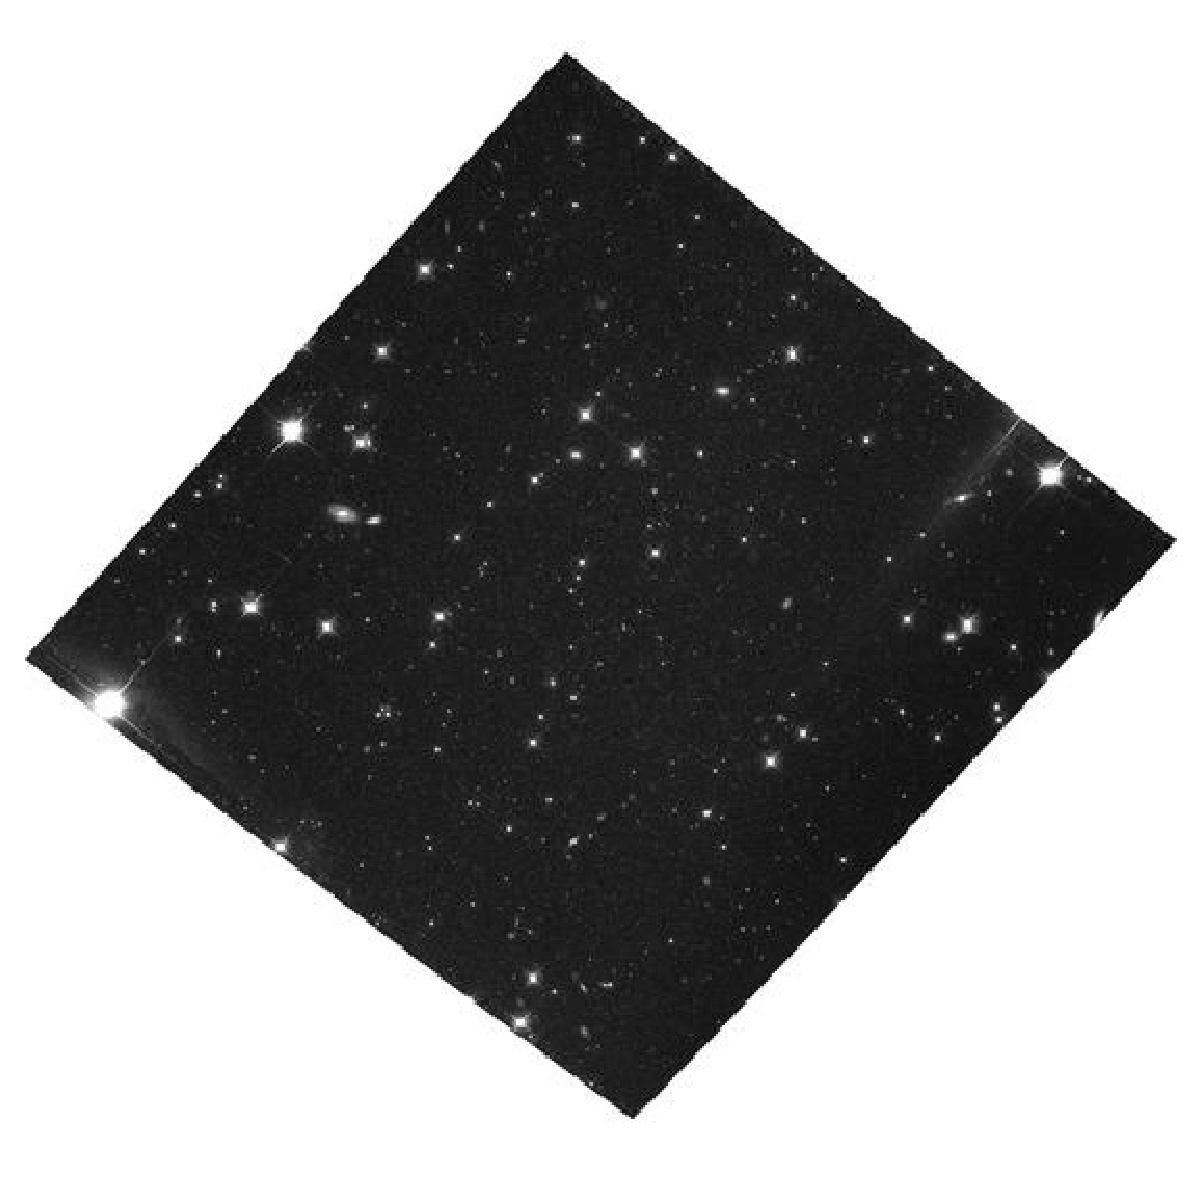
\includegraphics[width=0.18\textwidth]{\thedatafolder/img_tti_abs_1_1.pdf} \\ \input{\thedatafolder/propid_tti_abs_1_1.txt} & \centering 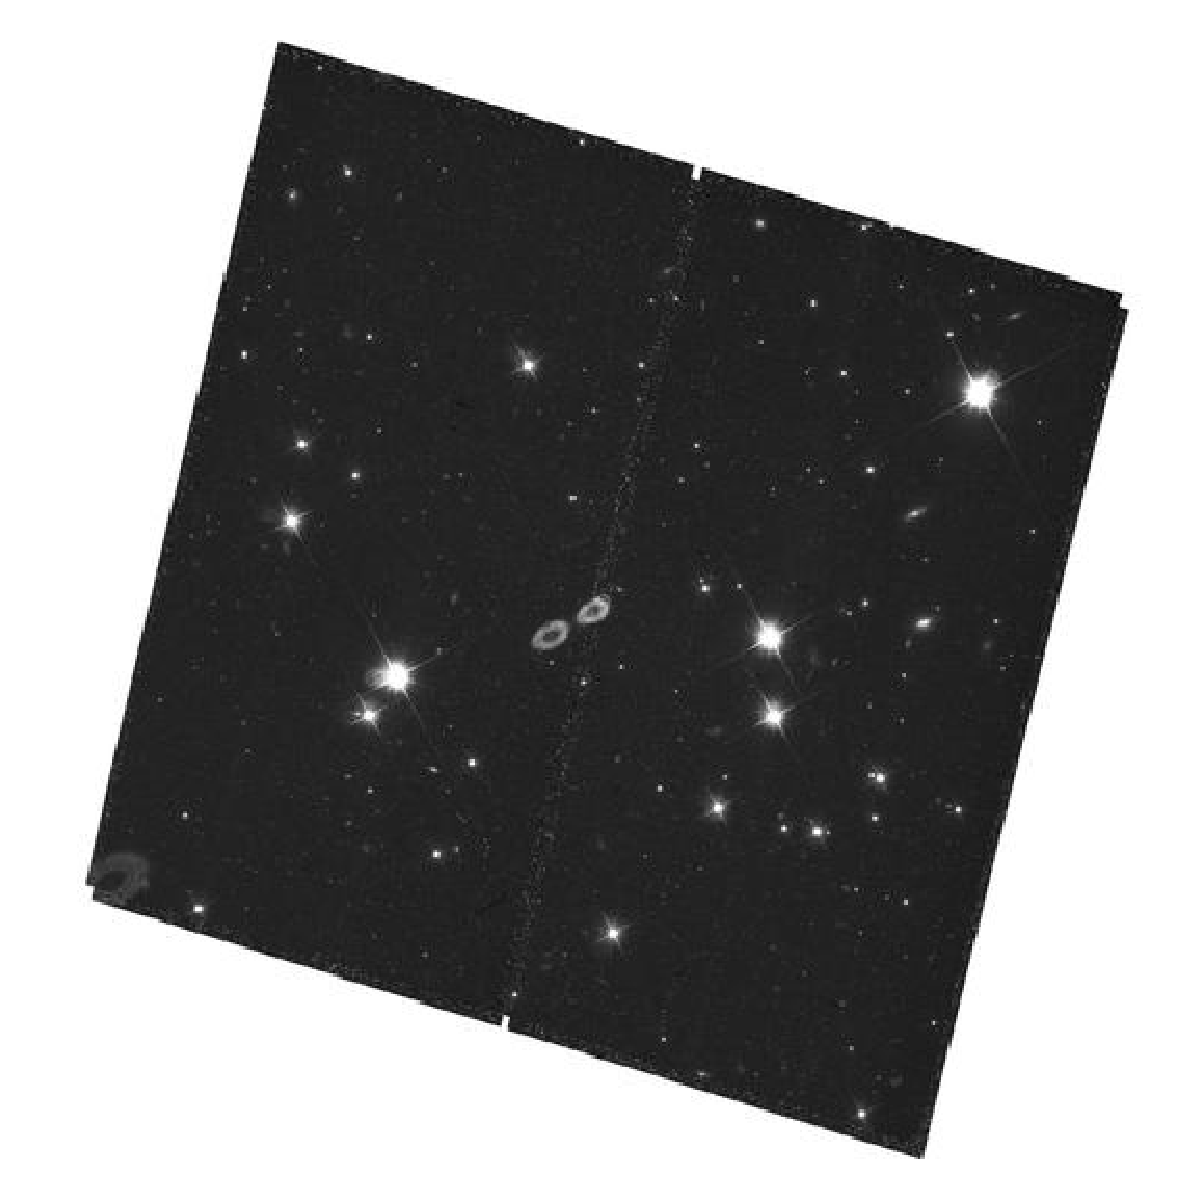
\includegraphics[width=0.18\textwidth]{\thedatafolder/img_tti_abs_1_2.pdf} \\ \input{\thedatafolder/propid_tti_abs_1_2.txt} & \centering \includegraphics[width=0.18\textwidth]{\thedatafolder/img_tti_abs_1_3.pdf} \\ \input{\thedatafolder/propid_tti_abs_1_3.txt}  \tabularnewline
      \midrule
      \texttt{\input{\thedatafolder/query_tti_abs_0.txt}} \vspace{20mm} & \centering \includegraphics[width=0.18\textwidth]{\thedatafolder/img_tti_abs_0_0.pdf} \\ \input{\thedatafolder/propid_tti_abs_0_0.txt} & \centering \includegraphics[width=0.18\textwidth]{\thedatafolder/img_tti_abs_0_1.pdf} \\ \input{\thedatafolder/propid_tti_abs_0_1.txt} & \centering \includegraphics[width=0.18\textwidth]{\thedatafolder/img_tti_abs_0_2.pdf} \\ \input{\thedatafolder/propid_tti_abs_0_2.txt} & \centering \includegraphics[width=0.18\textwidth]{\thedatafolder/img_tti_abs_0_3.pdf} \\ \input{\thedatafolder/propid_tti_abs_0_3.txt}  \tabularnewline
      \midrule
      \texttt{\input{\thedatafolder/query_tti_abs_2.txt}} \vspace{20mm} & \centering \includegraphics[width=0.18\textwidth]{\thedatafolder/img_tti_abs_2_0.pdf} \\ \input{\thedatafolder/propid_tti_abs_2_0.txt} & \centering \includegraphics[width=0.18\textwidth]{\thedatafolder/img_tti_abs_2_1.pdf} \\ \input{\thedatafolder/propid_tti_abs_2_1.txt} & \centering \includegraphics[width=0.18\textwidth]{\thedatafolder/img_tti_abs_2_2.pdf} \\ \input{\thedatafolder/propid_tti_abs_2_2.txt} & \centering \includegraphics[width=0.18\textwidth]{\thedatafolder/img_tti_abs_2_3.pdf} \\ \input{\thedatafolder/propid_tti_abs_2_3.txt}  \tabularnewline
      \midrule
      \texttt{\input{\thedatafolder/query_tti_abs_3.txt}} \vspace{20mm} & \centering \includegraphics[width=0.18\textwidth]{\thedatafolder/img_tti_abs_3_0.pdf} \\ \input{\thedatafolder/propid_tti_abs_3_0.txt} & \centering \includegraphics[width=0.18\textwidth]{\thedatafolder/img_tti_abs_3_1.pdf} \\ \input{\thedatafolder/propid_tti_abs_3_1.txt} & \centering \includegraphics[width=0.18\textwidth]{\thedatafolder/img_tti_abs_3_2.pdf} \\ \input{\thedatafolder/propid_tti_abs_3_2.txt} & \centering \includegraphics[width=0.18\textwidth]{\thedatafolder/img_tti_abs_3_3.pdf} \\ \input{\thedatafolder/propid_tti_abs_3_3.txt}  \tabularnewline
      \bottomrule
  \end{tabular}
  \caption{Same as Tabs.~\ref{tab:tti_base} and \ref{tab:tti}, but using the \textbf{\textcolor{deepblue}{abstract fine-tuned CLIP model}}.}
  \label{tab:tti_abs}
\end{table}

\begin{table}[t!]
  \centering
  \renewcommand{\arraystretch}{0.1}
  \begin{tabular}{m{3cm} m{3.9cm} m{3.9cm} m{3.9cm}}
      \toprule
      \centering \bfseries \hubble image & \centering \textbf{Top-4 text} \\ \textbf{\textcolor{deeppurple}{(base)}} & \centering  \textbf{Top-4 text} \\ \textbf{\textcolor{deepblue}{(abstract fine-tuned)}} & \centering  \textbf{Top-4 text} \\ \textbf{\textcolor{deepred}{(summary fine-tuned)}} \tabularnewline
      \midrule
      \centering \includegraphics[width=0.15\textwidth]{\thedatafolder/img_itt_abs_0.pdf} & \centering \scriptsize \verbatiminput{\thedatafolder/sci_itt_base_0.txt} & \centering  \scriptsize \verbatiminput{\thedatafolder/sci_itt_abs_0.txt} &  {\scriptsize \verbatiminput{\thedatafolder/sci_itt_0.txt}} \tabularnewline
      \midrule
      \centering \includegraphics[width=0.15\textwidth]{\thedatafolder/img_itt_abs_1.pdf} & \centering \scriptsize \verbatiminput{\thedatafolder/sci_itt_base_1.txt} & \centering  \scriptsize \verbatiminput{\thedatafolder/sci_itt_abs_1.txt} &  {\scriptsize \verbatiminput{\thedatafolder/sci_itt_1.txt}} \tabularnewline
      \midrule
      \centering \includegraphics[width=0.15\textwidth]{\thedatafolder/img_itt_abs_2.pdf} & \centering \scriptsize \verbatiminput{\thedatafolder/sci_itt_base_2.txt} & \centering  \scriptsize \verbatiminput{\thedatafolder/sci_itt_abs_2.txt} &  {\scriptsize \verbatiminput{\thedatafolder/sci_itt_2.txt}} \tabularnewline
      \midrule
      \centering \includegraphics[width=0.15\textwidth]{\thedatafolder/img_itt_abs_3.pdf} & \centering \scriptsize \verbatiminput{\thedatafolder/sci_itt_base_3.txt} & \centering  \scriptsize \verbatiminput{\thedatafolder/sci_itt_abs_3.txt} &  {\scriptsize \verbatiminput{\thedatafolder/sci_itt_3.txt}} \tabularnewline
      \bottomrule
  \end{tabular}
  \caption{Text associations from a curated list most closely matching four image queries (first column, the same as in Tab.~\ref{tab:itt}), for the \textcolor{deeppurple}{base} (CLIP-ViT-B/16), \textcolor{deepblue}{abstract fine-tuned}, and \textcolor{deepred}{summary fine-tuned} models.}
  \label{tab:itt_abs}
\end{table}
  
\end{document}
